%%=============================================================================
%% Onderzoek
%%=============================================================================

\chapter{Testen}
\label{ch:testen}

In dit hoofdstuk zullen de uitgevoerde experimenten en testen uiteengezet en besproken worden, volgens de richtlijnen aangehaald in Hoofdstuk~\ref{ch:methodologie}. Ze zullen gesorteerd staan volgens opstelling en gerangschikt in dezelfde volgorde als in Hoofdstuk~\ref{ch:opstellingen}.

\section{RFID}
Voor elk van volgende testen bestaat data over zowel de RSSI als het relatieve faseverschil. Het verloop van het relatieve faseverschil is gelijkaardig aan de RSSI, aangezien beide afhankelijk zijn van de afstand tussen de antenne en de tag. Alhoewel de grafieken van het relatieve faseverschil veelal een mooier verloop hebben, is er gekozen de conclusies van volgende testen te nemen op basis van de RSSI grafieken. Dit aangezien de relatieve fase een berekende waarde is, berekend uit het absolute faseverschil. Deze berekening is echter niet in alle gevallen volledig correct, waardoor er onvoorziene fenomenen zouden kunnen optreden in algoritmes gebaseerd op deze data. Echter is het in theorie mogelijk dezelfde conclusies te bekomen gebaseerd op de (correcte) relatieve fasedata.
Verder is er bij alle statische testen data over de in en de uit richting van de locatie, hiervan zal slechts 1 worden getoond aangezien beide richtingen dezelfde info verschaffen.
Alle volgende grafieken zijn gegenereerd door ARTA \footnote{Zie Sectie~\ref{sec:lit-software} op pagina~\pageref{sec:lit-software}}, waarin het helaas niet mogelijk is om een as te labelen. In alle RSSI grafieken vertegenwoordigd de x-as te tijd (in seconden) en de y-as de RSSI waarde (in dBm).

\subsection{1 antenne aan deurlijst}
\label{sec:ond-rfid-1}
\subsubsection{Deelhypothese}
Deze opstelling kan het voorbijkomen van een getagd asset waarnemen.

\subsubsection{Test: PoC}
\label{sec:ond-rfid-1-1}
Deze eerste en enige test voor deze opstelling is een proof of concept test. Hier wordt nagegaan of en hoe een voorbijkomende tag geregistreerd wordt. Voor de opstelling is 1 antenne gebruikt die vlak aan een deurkader is bevestigd. De tag komt vervolgens door het deurgat op een afstand van ~30 cm van de antenne voorbij, dit in een horizontale positie in een evenwijdig vlak aan de antenne.

\begin{minipage}{0.55\textwidth}
De grafiek in figuur~\ref{fig:ond-rfid-static-0-res} toon het resultaat van deze test. Hier is zichtbaar dat de reader een voorbijkomende tag registreert, en dit als een piek in de RSSI waarde.
\end{minipage}
\hfill
\begin{minipage}{0.42\textwidth}
	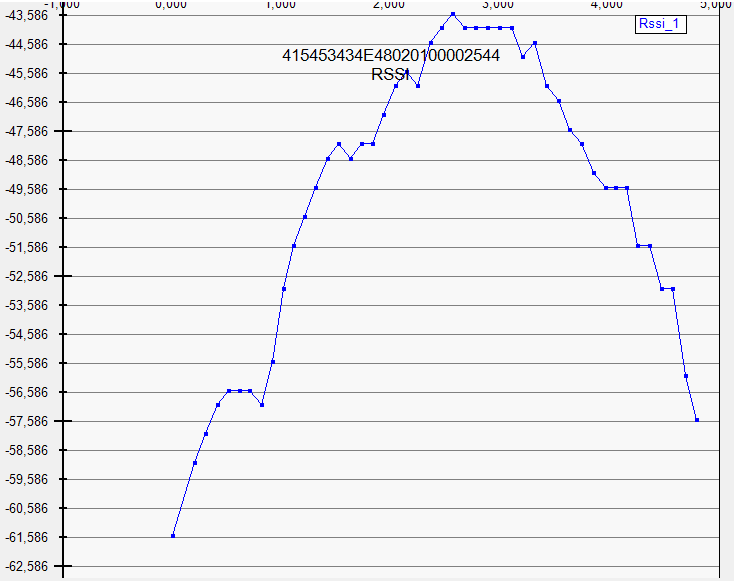
\includegraphics[width=\linewidth]{0_RSSI}
	\captionof{figure}{1 antenne aan deurlijst - Testresultaat}
	\label{fig:ond-rfid-static-0-res}
\end{minipage}

\subsubsection{Deelconclusie}
Uit deze test is duidelijk dat een voorbijkomende tag, en bij uitbreiding een getagd asset, die de locatie binnenkomt, waargenomen wordt. De deelhypothese is aangenomen. Buiten deze simpele registratietest is er ook nood aan het testen van de invloed van de oriëntatie en afstand van de tag tegenover de antenne. Deze fenomenen gelden ook voor een opstelling met 2 antennes, en worden bijgevolg onderzocht in de respectievelijke testen in sectie~\ref{sec:ond-rfid-2}.

\subsection{2 antennes aan deurlijst}
\label{sec:ond-rfid-2}
\subsubsection{Deelhypothese}
Deze opstelling kan het voorbijkomen en de richting van een getagd asset waarnemen, genomen dat de afstand tussen de tag en de antenne voldoende klein is.

\subsubsection{Test 1: Oriëntatie van de tag}
\label{sec:ond-rfid-2-1}
In deze eerste test wordt de invloed van de oriëntatie van de tag tegenover de antennes bepaald, aangezien deze oriëntatie in theorie een invloed heeft op de gemeten RSSI waarde\footnote{Zie 'RSSI beïnvloedende factoren' in Sectie~\ref{subsec:lit-rfid} op pagina~\pageref{subsec:lit-rfid}}. De opstelling voor deze test is als volgt: Tegen een deurlijst zijn 2 antennes naast elkaar geplaatst. Bij het binnenkomen wordt eerst antenne 1, en daarna antenne 2 gepasseerd. Er worden 4 oriëntaties onderzocht, nl. horizontaal (a) en verticaal (b) in een evenwijdig vlak aan de antennes, en horizontaal (c) en verticaal (d) loodrecht op het vlak van de antennes. Deze tag komt door het deurgat op een afstand van ~30 cm van de antennes voorbij.
In theorie zouden a en b ruwweg dezelfde resultaten moeten geven, terwijl c en d een lagere RSSI zouden moeten geven. Echter zou de voorbij komst van de tags in elk geval detecteerbaar moeten zijn.

\paragraph{a) Horizontaal in antennevlak}
\begin{minipage}{0.55\textwidth}
De grafiek in figuur~\ref{fig:ond-rfid-static-1a-res} toon het resultaat van deze deeltest, in de uitgaande richting. Er is duidelijk een opeenvolging van pieken zichtbaar. Dit met volgorde 2 (groen) -> 1 (blauw), wat inderdaad betekend dat de tag uit de locatie gaat. De detectie is geslaagd. De piekhoogtes zijn niet gelijk, ondanks dat de antennes hetzelfde type zijn. Dit is kalibreerbaar maar zoals zichtbaar is dit niet nodig voor een toepassing als deze.
\end{minipage}
\hfill
\begin{minipage}{0.42\textwidth}
	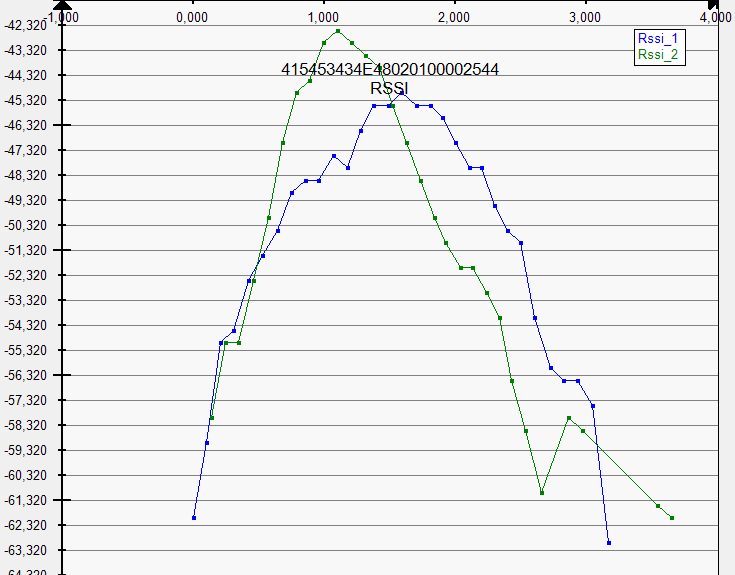
\includegraphics[width=\linewidth]{1a_uit_RSSI}
	\captionof{figure}{2 antennes aan deurlijst - Testresultaat 1a}
	\label{fig:ond-rfid-static-1a-res}
\end{minipage}

\paragraph{b) Verticaal in antennevlak}
\begin{minipage}{0.55\textwidth}
De grafiek in figuur~\ref{fig:ond-rfid-static-1b-res} toon het resultaat van deze deeltest, in de uitgaande richting. Ze is vrij gelijkaardig aan de vorige, wat theoretisch ook zou moeten. Er zijn duidelijk 2 pieken zichtbaar, in de juiste volgorde volgens de tag die uit de locatie gaat. Ook is de RSSI gelijkaardig (rond de -40 à -45 dBm).
\end{minipage}
\hfill
\begin{minipage}{0.42\textwidth}
	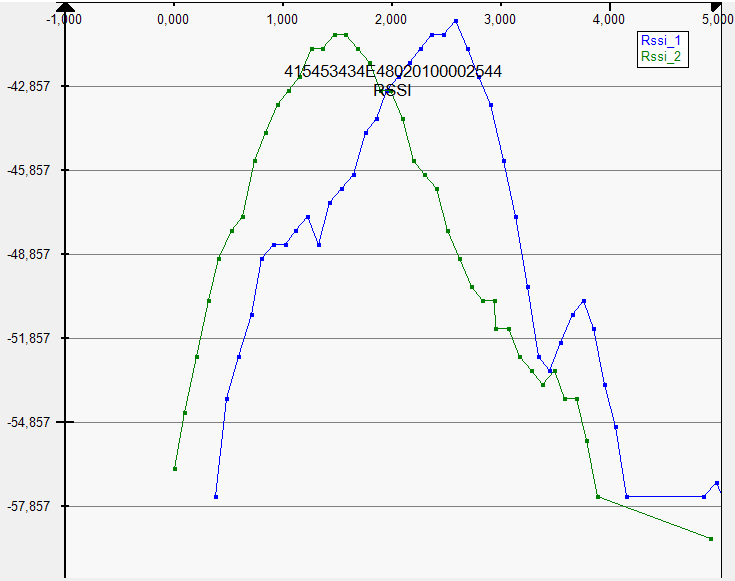
\includegraphics[width=\linewidth]{1b_uit_RSSI}
	\captionof{figure}{2 antennes aan deurlijst - Testresultaat 1b}
	\label{fig:ond-rfid-static-1b-res}
\end{minipage}

\paragraph{c) Horizontaal loodrecht op antennevlak}
\begin{minipage}{0.55\textwidth}
De grafiek in figuur~\ref{fig:ond-rfid-static-1c-res} toon het resultaat van deze deeltest, in de binnenkomende richting. De toppen zijn noch steeds duidelijk zichtbaar, en ze staan in de correcte richting, maar de top is iets minder duidelijk afgelijnd en meer uitgerokken. Ditzelfde fenomeen is ook zichtbaar in de uit-richting. Ook liggen de toppen iets lager dan de toppen in de vorige 2 deeltests.
\end{minipage}
\hfill
\begin{minipage}{0.42\textwidth}
	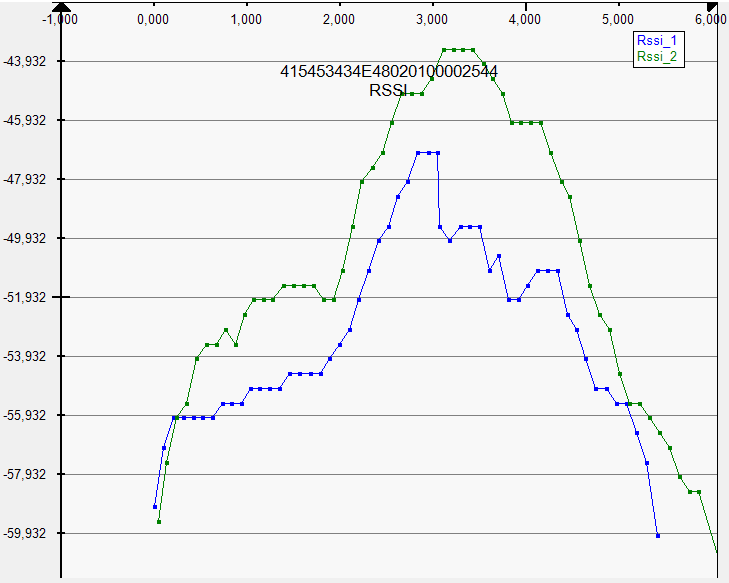
\includegraphics[width=\linewidth]{1c_in_RSSI}
	\captionof{figure}{2 antennes aan deurlijst - Testresultaat 1c}
	\label{fig:ond-rfid-static-1c-res}
\end{minipage}

\paragraph{d) Verticaal loodrecht op antennevlak}
\begin{minipage}{0.55\textwidth}
De grafiek in figuur~\ref{fig:ond-rfid-static-1d-res} toon het resultaat van deze deeltest, in de binnenkomende richting. Hier is het fenomeen van meer uitgerokken toppen nog beter zichtbaar. De uit richting vertoont wederom hetzelfde patroon. Deze deeltest ligt in lijn met de vorige, maar nog opvallender.
\end{minipage}
\hfill
\begin{minipage}{0.42\textwidth}
	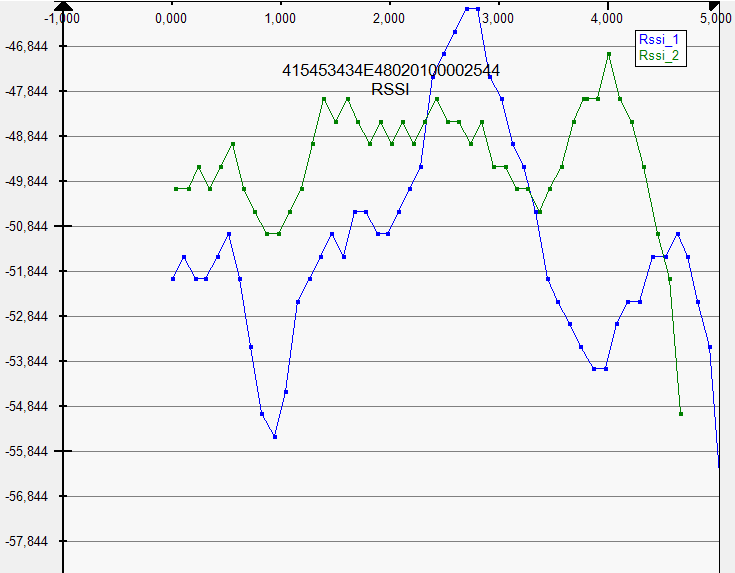
\includegraphics[width=\linewidth]{1d_in_RSSI}
	\captionof{figure}{2 antennes aan deurlijst - Testresultaat 1d}
	\label{fig:ond-rfid-static-1d-res}
\end{minipage}

\paragraph{Testconclusie}
Zoals verwacht is de detectie van de tag en de richting ervan goed zichtbaar en in elk geval correct gemeten. Ook is de meetkwaliteit minder als de tags niet in het vlak van de antenne liggen, daarom lijkt het aanbevolen dit zo veel mogelijk te vermijden.

\subsubsection{Test 2: Afstand tussen tag en antennes}
\label{sec:ond-rfid-2-2}
In deze test wordt de invloed van de afstand tussen de tag en de antennes gemeten, in theorie zou de RSSI van de piek lager moeten zijn als de tag verder van de antenne voorbij komt. Ook zouden, door de conische vorm van het meetveld van de vlakke antenne\footnote{Zie Sectie~\ref{sec:met-rfid} op pagina~\pageref{sec:met-rfid}}, de pieken meer moeten overlappen. De testopstelling is idem aan Test 1. De oriëntatie van de tag is constant gehouden op horizontaal in hetzelfde vlak als de antennes, en de richting is uitgaand. De gemeten afstanden zijn 5cm (zeer dicht) en 100cm (zeer ver). Deze resultaten worden vergeleken met de resultaten van Test 1a, aangezien dit dezelfde opstelling betreft, op 30 cm afstand.

\paragraph{a) 5cm}
\begin{minipage}{0.55\textwidth}
Op de grafiek in figuur~\ref{fig:ond-rfid-static-2a-res} is het verwachte resultaat te zien, 2 duidelijke pieken die licht verder uit elkaar liggen, en een hogere RSSI waarde hebben.
\end{minipage}
\hfill
\begin{minipage}{0.42\textwidth}
	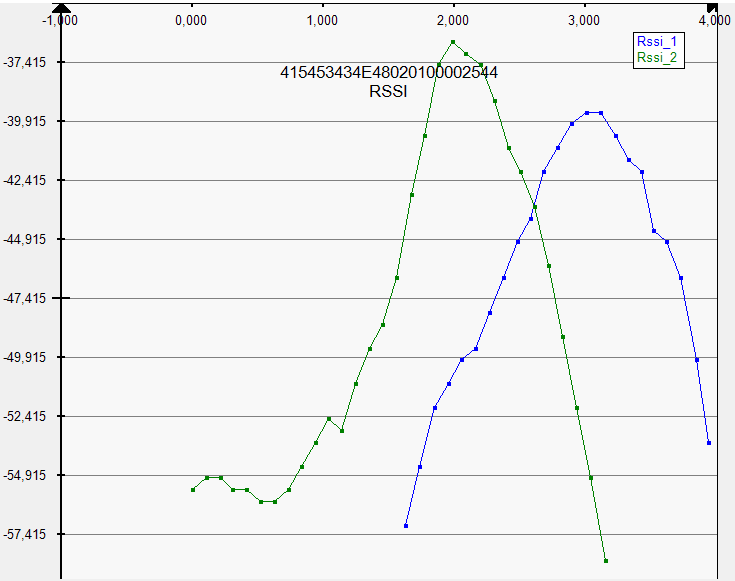
\includegraphics[width=\linewidth]{2a_RSSI}
	\captionof{figure}{2 antennes aan deurlijst - Testresultaat 2a}
	\label{fig:ond-rfid-static-2a-res}
\end{minipage}

\paragraph{b) 100cm}
\begin{minipage}{0.55\textwidth}
De grafiek in figuur~\ref{fig:ond-rfid-static-2b-res} toon het resultaat van deze deeltest, en is interessanter dan de vorige. Het vermoeden dat de piek minder duidelijk ging zijn en ging overlappen is bevestigd. Uit deze meting kan niet meer afgeleid worden in welke richting de tag voorbij de antennes komt. Ook ligt de RSSI waarde beduidend lager.
\end{minipage}
\hfill
\begin{minipage}{0.42\textwidth}
	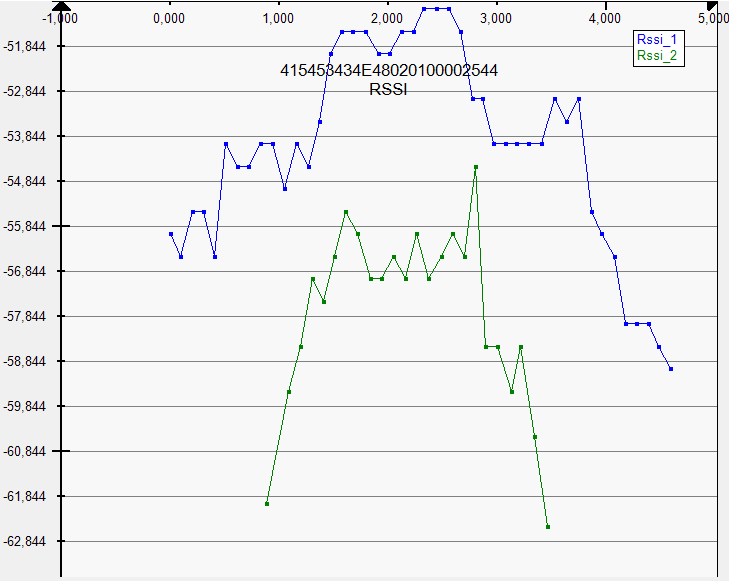
\includegraphics[width=\linewidth]{2b_RSSI}
	\captionof{figure}{2 antennes aan deurlijst - Testresultaat 2b}
	\label{fig:ond-rfid-static-2b-res}
\end{minipage}

\paragraph{Testconclusie}
Er bestaat duidelijk een bepaalde restrictie op de afstand waarmee de tag de antennes kan voorbijkomen om een goede richtingsdetectie te hebben. 

\subsubsection{Test 3: Afstand tussen de 2 antennes}
\label{sec:ond-rfid-2-3}
Aangezien de reden van de overlappende pieken in test 2 het feit is dat het conische bereik van de 2 antennes elkaar te veel overlapt, is het logisch dat dit effect zal verminderen als deze 2 antennes verder van elkaar geplaatst worden. Dit zal getest worden in deze 3e test. De opstelling is identiek aan deze in test 2, met als enige verschil dat de 2 antennes 20cm uit elkaar geplaatst zijn.

\paragraph{a) 5cm}
\begin{minipage}{0.55\textwidth}
De grafiek in figuur~\ref{fig:ond-rfid-static-3a-res} toon het resultaat van deze deeltest. Deze toont wederom 2 mooie pieken, deze keer iets verder uit elkaar liggend door de afstand tussen de antennes, en dit met een hoge RSSI waarde.
\end{minipage}
\hfill
\begin{minipage}{0.42\textwidth}
	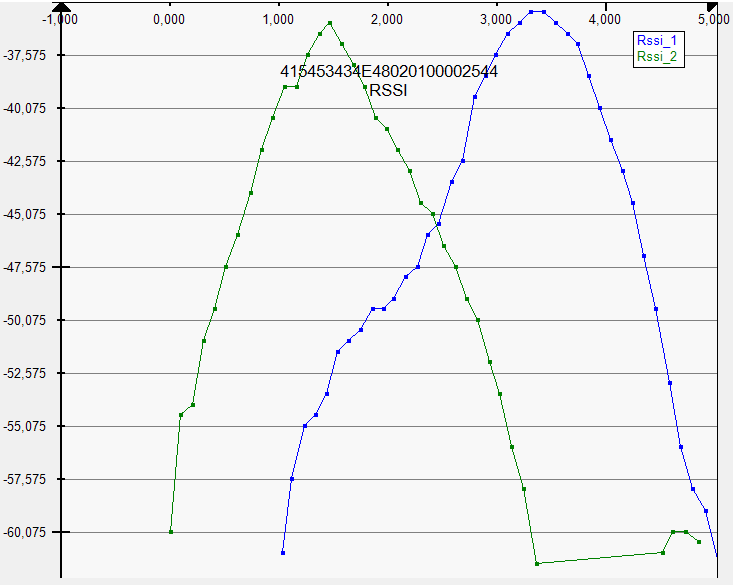
\includegraphics[width=\linewidth]{3a_RSSI}
	\captionof{figure}{2 antennes aan deurlijst - Testresultaat 3a}
	\label{fig:ond-rfid-static-3a-res}
\end{minipage}

\paragraph{b) 30cm}
\begin{minipage}{0.55\textwidth}
De grafiek in figuur~\ref{fig:ond-rfid-static-3b-res} toon het resultaat van deze deeltest. Ze vertoont een gelijkaardig beeld aan de vorige, enkel licht meer uitgerokken en met een lagere RSSI waarde dan bij 5 cm.
\end{minipage}
\hfill
\begin{minipage}{0.42\textwidth}
	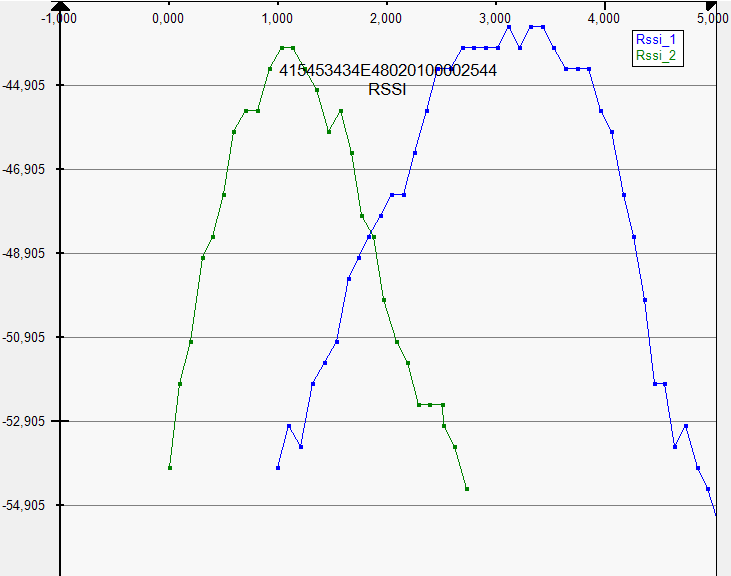
\includegraphics[width=\linewidth]{3b_RSSI}
	\captionof{figure}{2 antennes aan deurlijst - Testresultaat 3b}
	\label{fig:ond-rfid-static-3b-res}
\end{minipage}

\paragraph{c) 100cm}
\begin{minipage}{0.55\textwidth}
Dit resultaat, zichtbaar in de grafiek in figuur~\ref{fig:ond-rfid-static-3c-res}, is de voornaamste van deze test. Er is zoals bij test 2 te zien dat de pieken weer hard zijn uitgerokken, maar door de extra afstand tussen de antennes is de volgorde wel weer zichtbaar.
\end{minipage}
\hfill
\begin{minipage}{0.42\textwidth}
	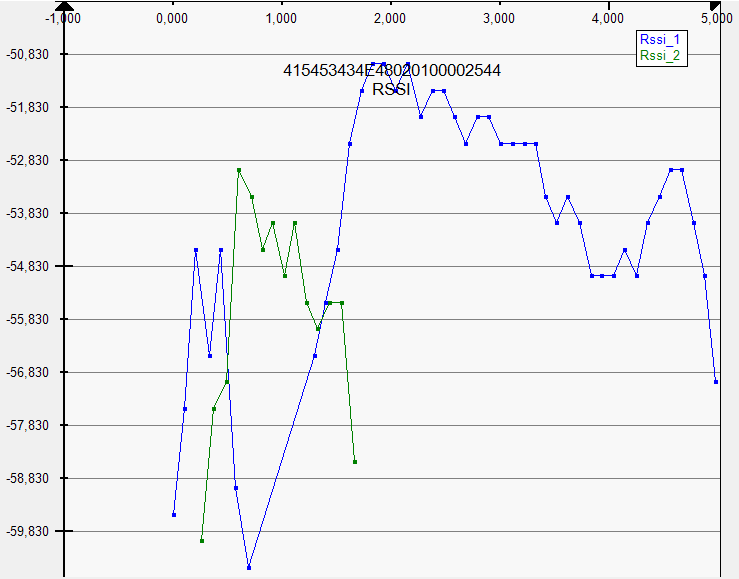
\includegraphics[width=\linewidth]{3c_RSSI}
	\captionof{figure}{2 antennes aan deurlijst - Testresultaat 3c}
	\label{fig:ond-rfid-static-3c-res}
\end{minipage}

\paragraph{Testconclusie}
Het blijkt inderdaad correct dat het verder uit elkaar plaatsen van de antennes een positief effect heeft op het uit elkaar trekken van de pieken van de RSSI curves. Hieruit blijkt dat extra afstand tussen de antennes nuttig is voor richtingsdetectie als de tags op grotere afstand voorbij komen.

\subsubsection{Deelconclusie}
Deze opstelling slaagt er inderdaad in om een voorbijkomende tag en zijn richting te registreren, mits de afstand beperkt is. De deelhypothese is aangenomen. Er kan echter wel aan toegevoegd worden dat, als de afstand niet meer voldoende klein is, de afstand tussen de antennes kan vergroot worden. Dit is in een reële situatie echter niet praktisch aangezien een deur meestal een beperkte breedte heeft. Voor een standaard deur zal dit geen probleem zijn aangezien de maximale afstand in een deur ook beperkt is, maar voor bv. een poortdoorgang kan dit wel problemen opleveren. In een gang met een quasi onbeperkte beschikbare breedte is dit wel mogelijk.

\subsection{1 antenne tegenover deur}
\label{sec:ond-rfid-3}
\subsubsection{Deelhypothese}
Deze opstelling kan het voorbijkomen en de richting van een getagd asset waarnemen, genomen dat de afstand tussen de antenne en de deur voldoende klein is.

\subsubsection{Test 1: PoC}
\label{sec:ond-rfid-3-1}
Deze eerste test bestaat uit een proof of concept, hierin wordt getest of het op zijn minst mogelijk is om de richting van de bewegende tag te bepalen uit de gemeten data. 
Voor de testopstelling is een antenne geplaatst tegen een muur. Voor deze muur bevind zich een kar met een tag op (horizontaal in het vlak evenwijdig aan de antenne). Deze kar word weg van en naar de antenne toe gerold.

\paragraph{Resultaat}
De grafieken in figuren~\ref{fig:ond-rfid-static-4c-res} en ~\ref{fig:ond-rfid-static-4d-res}  tonen de verandering in RSSI in beide richtingen. Dit met het rollen van de kar weg van de antenne links, en naar de antenne toe rechts. In deze grafieken is deze richting zeer mooi zichtbaar, de RSSI verlaagt als de kar wegrolt, en verhoogt als deze naar de antenne toe rolt.

\begin{minipage}{0.42\textwidth}
	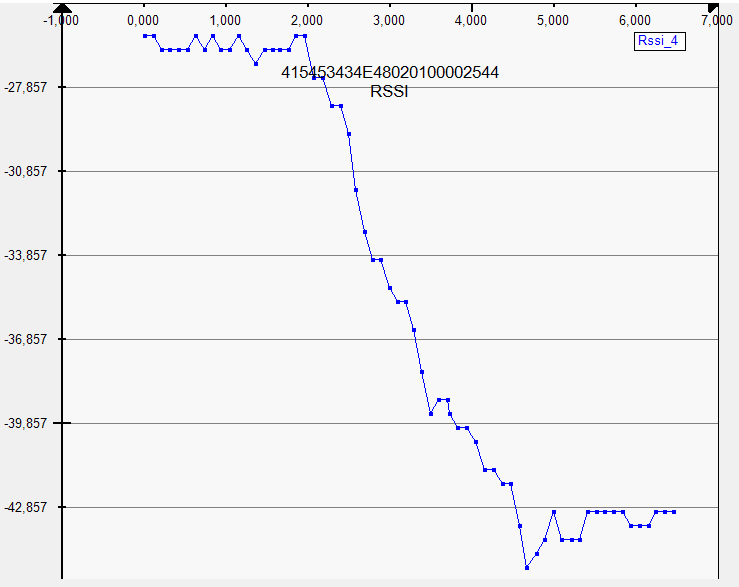
\includegraphics[width=\linewidth]{4c_RSSI}
	\captionof{figure}{1 antenne tegenover deur - Testresultaat 1 uit}
	\label{fig:ond-rfid-static-4c-res}
\end{minipage}
\hfill
\begin{minipage}{0.42\textwidth}
	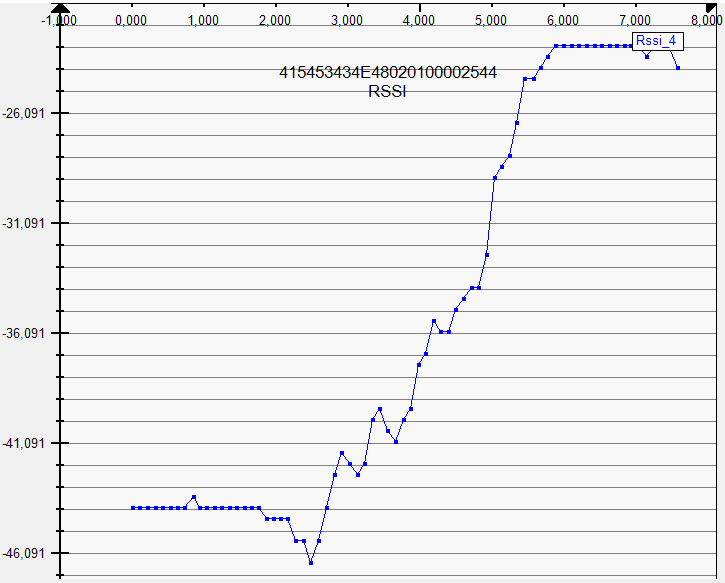
\includegraphics[width=\linewidth]{4d_RSSI}
	\captionof{figure}{1 antenne tegenover deur - Testresultaat 1 in}
	\label{fig:ond-rfid-static-4d-res}
\end{minipage}

\paragraph{Testconclusie}
Uit deze resultaten is de rijrichting van de kar zeer mooi afleidbaar, mits ze op de lijn voor de antenne rijd.

\subsubsection{Test 2: Variabele afstand tot deur}
\label{sec:ond-rfid-3-2}
In deze test wordt de opstelling realistischer gemaakt. Bij deze test staat de antenne op respectievelijk 100 en 200 cm afstand van de deur. Vervolgens rijd de met RFID tag voorziene kar uit test 1 door de deur. Dit direct de hoek om, zowel in als uit de kamer.

\paragraph{a) 100cm}
In de grafieken in figuren~\ref{fig:ond-rfid-static-5ain-res} en ~\ref{fig:ond-rfid-static-5auit-res} is het binnenkomen (links) en het verlaten (rechts) van de locatie te zien. Het is meteen duidelijk dat de rijrichting in dit scenario veel minder duidelijk af te lijden is dan bij de vorige test. Vermoedelijk is de 'staart' die niet in de meting past (rechts aanhangsel bij inwaarts en links bij uitwaarts) het gevolg van het feit dat de kar op dat moment 90° gedraaid in de kamer aanwezig is, resp. na en voor de draaibeweging door de deur. Op dit moment bevind de tag zich in het leesveld van de antenne, maar niet meer in een evenwijdig vlak. Deze onderlinge oriëntatie zorgt voor een slechtere RSSI waarde, zoals aangetoond tijdens test 1 in sectie~\ref{sec:ond-rfid-2}. Voor de duidelijkheid van de 'uit' meting is dit niet zo zeer een probleem, maar wel voor de 'in' meting.

\begin{minipage}{0.42\textwidth}
	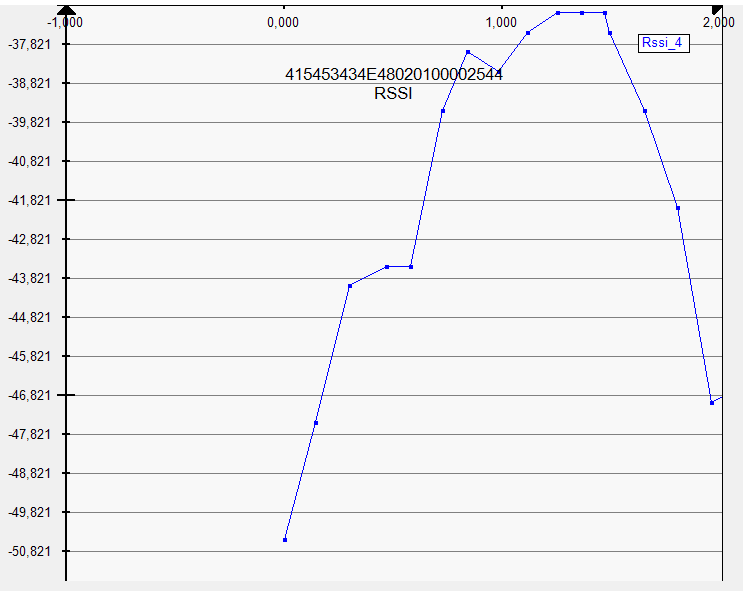
\includegraphics[width=\linewidth]{5a_in_RSSI}
	\captionof{figure}{1 antenne tegenover deur - Testresultaat 2a in}
	\label{fig:ond-rfid-static-5ain-res}
\end{minipage}
\hfill
\begin{minipage}{0.42\textwidth}
	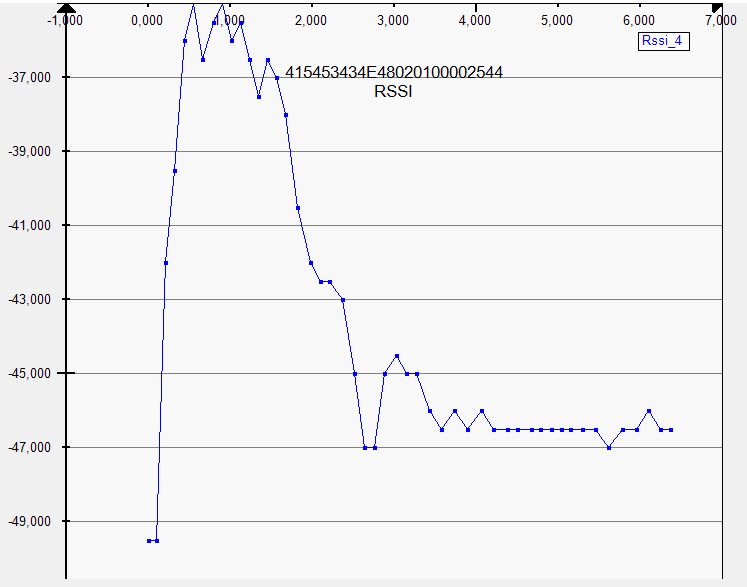
\includegraphics[width=\linewidth]{5a_uit_RSSI}
	\captionof{figure}{1 antenne tegenover deur - Testresultaat 2a uit}
	\label{fig:ond-rfid-static-5auit-res}
\end{minipage}

\paragraph{b) 200cm}
In de grafieken in figuren~\ref{fig:ond-rfid-static-5bin-res} en ~\ref{fig:ond-rfid-static-5buit-res} is wederom het binnenkomen (links) en het verlaten (rechts) van de locatie te zien. In dit geval is de onduidelijkheid, zichtbaar in vorige deeltest, nog extremer zichtbaar. Het is nog steeds mogelijk de richting af te leiden uit de resultaten, maar het wordt onduidelijker en dubbelzinniger. Deze onduidelijkheid vergroot vermoedelijk ook naarmate de tussenliggende afstand groter wordt. Ook de RSSI waarde ligt logischerwijs lager.

\begin{minipage}{0.42\textwidth}
	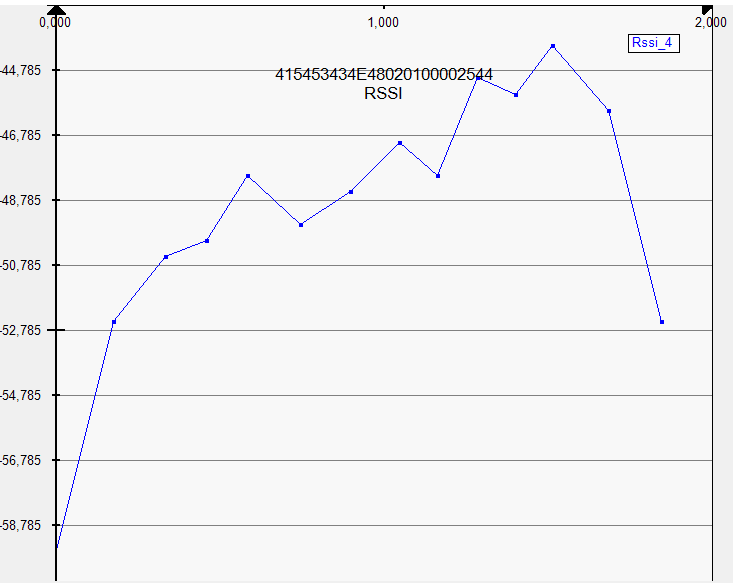
\includegraphics[width=\linewidth]{5b_in_RSSI}
	\captionof{figure}{1 antenne tegenover deur - Testresultaat 2b in}
	\label{fig:ond-rfid-static-5bin-res}
\end{minipage}
\hfill
\begin{minipage}{0.42\textwidth}
	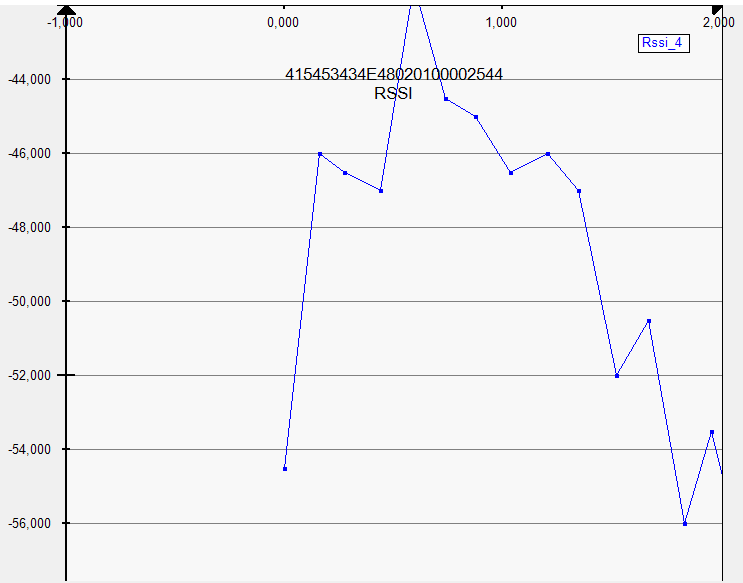
\includegraphics[width=\linewidth]{5b_uit_RSSI}
	\captionof{figure}{1 antenne tegenover deur - Testresultaat 2b uit}
	\label{fig:ond-rfid-static-5buit-res}
\end{minipage}

\paragraph{Testconclusie}
Deze testen tonen aan dat de meting in een realistisch scenario veel minder optimaal is als in het optimaal scenario van test 1. Dit omdat de meetpunten die niet het dichter of verder gaan van de antenne beschrijven voor onduidelijkheden zorgen die niet eenduidig uit de data te halen zijn.

\subsubsection{Test 3: Langere meetafstand}
\label{sec:ond-rfid-3-3}
Aangezien een simpele draai rond het deurgat te slechte data oplevert om eenduidig de richting te bepalen (zie test 2), kan het een idee zijn om de kar langer op de lijn voor de antenne te laten rijden. Hierdoor zal het relatieve aantal meetpunten voor de richtingsdetectie opgekrikt worden tegenover het aantal meetpunten bij het in- en uit stappen van deze lijn voor de antenne. Dit wordt in deze test bekeken, hierbij is de opstelling idem aan test 2b, maar zal de kar tot tegen de antenne rijden alvorens af te slaan.

\paragraph{Resultaat}
De grafieken in figuren~\ref{fig:ond-rfid-static-5cin-res} en ~\ref{fig:ond-rfid-static-5cuit-res} tonen wederom de verandering in RSSI van beide richtingen, met het rollen van de kar naar de antenne links, en weg van de antenne rechts. Alhoewel de 'staarten' uit test 2 nog steeds zichtbaar zijn, overheersen ze de grafiek niet meer en is deze grafiek veel eenduidiger. Hieruit  kan de richting van verplaatsing worden afgeleid uit de richting van de scheefheid van de grafiek.

\begin{minipage}{0.42\textwidth}
	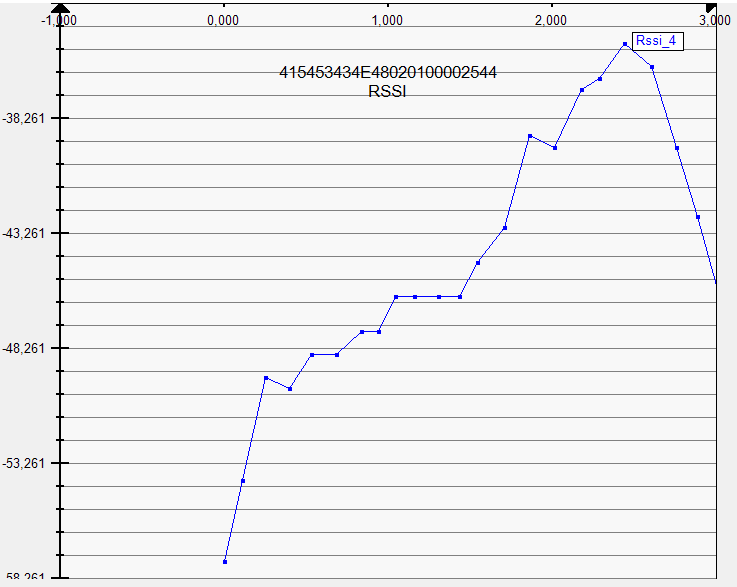
\includegraphics[width=\linewidth]{5c_in_RSSI}
	\captionof{figure}{1 antenne tegenover deur - Testresultaat 3 in}
	\label{fig:ond-rfid-static-5cin-res}
\end{minipage}
\hfill
\begin{minipage}{0.42\textwidth}
	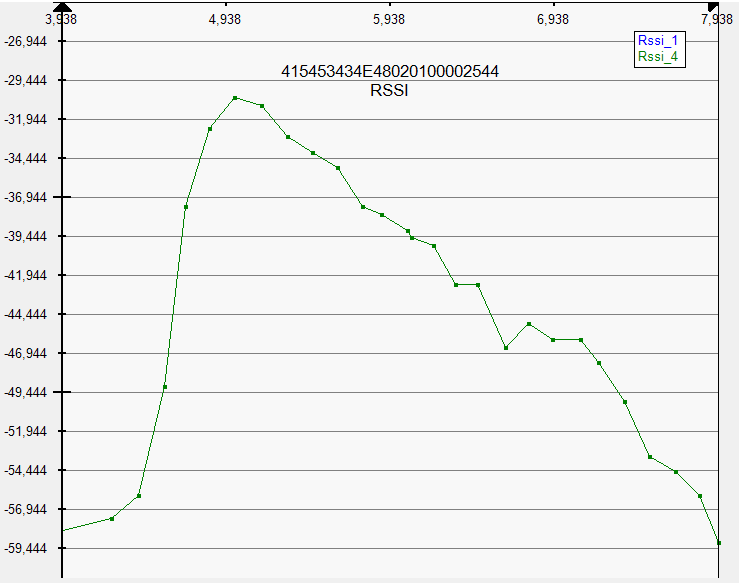
\includegraphics[width=\linewidth]{5c_uit_RSSI}
	\captionof{figure}{1 antenne tegenover deur - Testresultaat 3 uit}
	\label{fig:ond-rfid-static-5cuit-res}
\end{minipage}

\paragraph{Testconclusie}
Het vermoeden dat de resultaten beter zijn als er langer op de lijn voor de antenne wordt gewandeld lijkt te zijn bevestigd met deze test.

\subsubsection{Deelconclusie}
In ideale omstandigheden blijkt dit concept zeer goed te werken. Echter zijn er enkele neveneffecten van een realistische draai door een deur die moeten gecompenseerd worden met een langere lengte op de lijn voor de antenne te lopen. De vooropgestelde deelhypothese is verworpen en moet aangevuld worden met deze nieuwe informatie om te kunnen worden aangenomen. In praktijk wilt dit zeggen dat dit niet werkt voor een normale deuropening en de opstelling uit sectie~\ref{sec:ond-rfid-2} zal moeten gebruikt worden. Echter kan het wel een oplossing zijn voor een (korte) gang of dergelijke waar de assets sowieso door moeten om een berging of magazijn te bereiken, want vanaf er enige afstand wordt gedaan naar of weg van de antenne werkt deze opstelling wel zeer goed, met een lagere hardware kost. 

\subsection{1 tag aan deurlijst}
\label{sec:ond-rfid-4}
\subsubsection{Deelhypothese}
Deze opstelling is in staat om verspreide, getagde assets te detecteren en eenduidig aan de correcte locatie toe te wijzen.

\subsubsection{Test 1: Ideale situatie}
\label{sec:ond-rfid-4-1}
De opstelling voor deze test is als volgt: Een rijdende kar is voorzien van een RFID-reader, voorzien van een vlakke antenne, welke opzij (rechts) is gericht. Verder is er een een locatie, bestaande uit 1 ommuurde ruimte, deze is voorzien van 1 locatie tag (Tagcode 4) aan het deurframe, langs de rechterkant. Dit zodat de antenne op de kar de tag kan lezen bij het binnenkomen. Vervolgens bevinden zich verspreid over deze ruimte 4 assets, getagd met een asset tag (Tagcode 1, 2, 3 en 5). Als laatste is er aan de linkerkant van de deurlijst ook een locatie tag (Tagcode 6) aangebracht, voor een andere locatie dan deze. In en opstelling in productie zou deze aan de deur van een nieuwe locatie hangen, maar in deze opstelling is zijn functie louter om aan te geven wanneer de locatie wordt verlaten. Alle tags (zowel locatie als asset) bevinden zich op dezelfde hoogte als de antenne op de kar. De test is geslaagd als alle asset tags gemeten worden tussen het meten van de locatie tag van de locatie zelf eenderzijds en, en de tag van de andere locatie anderzijds.

\paragraph{Resultaat}
De resultaten van deze test zijn ondergebracht in grafiek~\ref{fig:ond-rfid-dynamic-6a-res}. Met leesbaarheid in gedachten zijn de tijdspannen tussen de registraties van de tags weggelaten uit de grafiek. In praktijk liggen deze verder uit elkaar in de tijd, maar voor deze test is voornamelijk de volgorde van belang. Deze resultaten tonen zeer duidelijk dat deze test geslaagd is, de reader registreert eerst tag 4, welke duidelijk maakt dat deze zich vanaf hier binnen de locatie bevindt. Elke asset tag die tussen deze locatie tag en de volgende locatie tag wordt gedetecteerd, bevindt zich in deze locatie. De 2e locatie tag is de laatste die wordt gedetecteerd, waardoor het duidelijk is dat deze test correct bepaald heeft dat alle assets zich op deze locatie bevinden. Wel is er een groot verschil merkbaar in het aantal meetpunten. Tag 5 wordt maar 2x gedetecteerd, in vergelijking tot de meer dan 50 meetpunten voor tag 3. Dit is echter niet geheel verrassend, aangezien het asset met tag 5 zich veel dieper in de kamer bevind dan deze met tag 3.

\begin{figure}[h]
	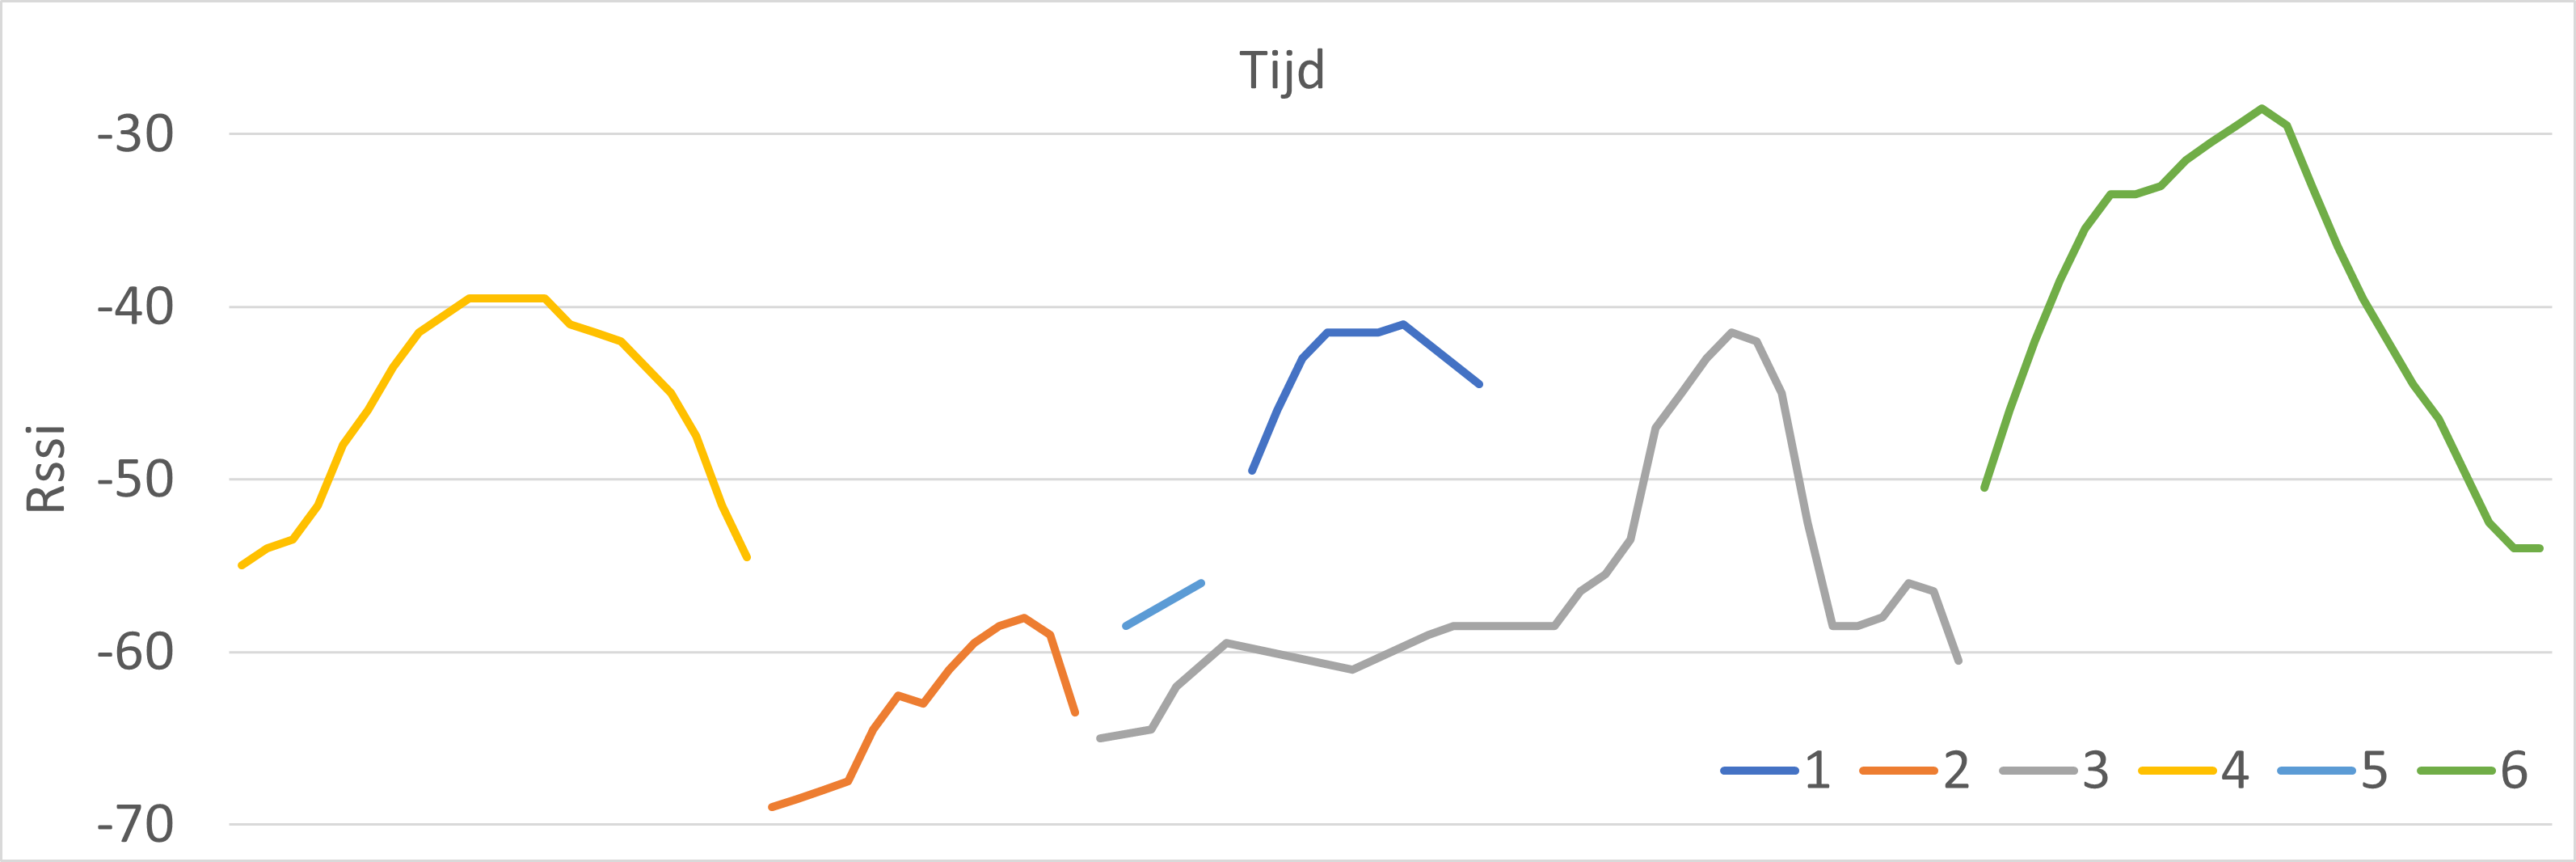
\includegraphics[width=\linewidth]{6a_RSSI}
	\caption{1 tag aan deurlijst - Testresultaat 1}
	\label{fig:ond-rfid-dynamic-6a-res}
\end{figure}

\paragraph{Testconclusie}
Het doel van de test, namelijk het detecteren van alle assets en ze correct plaatsen in de locatie, is geslaagd. Het feit dat er een groot verschil bestaat in het aantal meet- of detectiepunten wekt wel het vermoeden dat het voornaamste probleem met dit scenario zal liggen in het detecteren van alle aanwezige assets, en niet zo zeer in het bekomen van een correcte lokalisatie.

\subsubsection{Test 2: Realistische situatie}
\label{sec:ond-rfid-4-2}
Het is natuurlijk geen gegeven dat alle asset tags zich ook op ruwweg dezelfde hoogte als de antenne zullen bevinden. Dit aangezien de assets zelf zich in theorie overal in de kamer kunnen bevinden, inclusief op tafels of kasten. Deze test zal dezelfde opstelling nemen als de vorige test, maar de assets zullen zich ook op verschillende hoogtes bevinden.

\paragraph{Resultaat}
Dit resultaat, zichtbaar in grafiek~\ref{fig:ond-rfid-dynamic-6b-res}, toont de vrees van vorige test aan. De detectie is helaas veel slechter als de tags niet op het niveau van de antenne liggen. Er is geen probleem qua lokalisatie, aangezien de volgorde van de tags is nog steeds correct is. Echter is bij elke asset tag het aantal meet- of detectiepunten afgenomen en is de RSSI gezakt. Tag 5 is zelfs volledig verdwenen uit de data en is niet gedetecteerd.
\begin{figure}[h]
	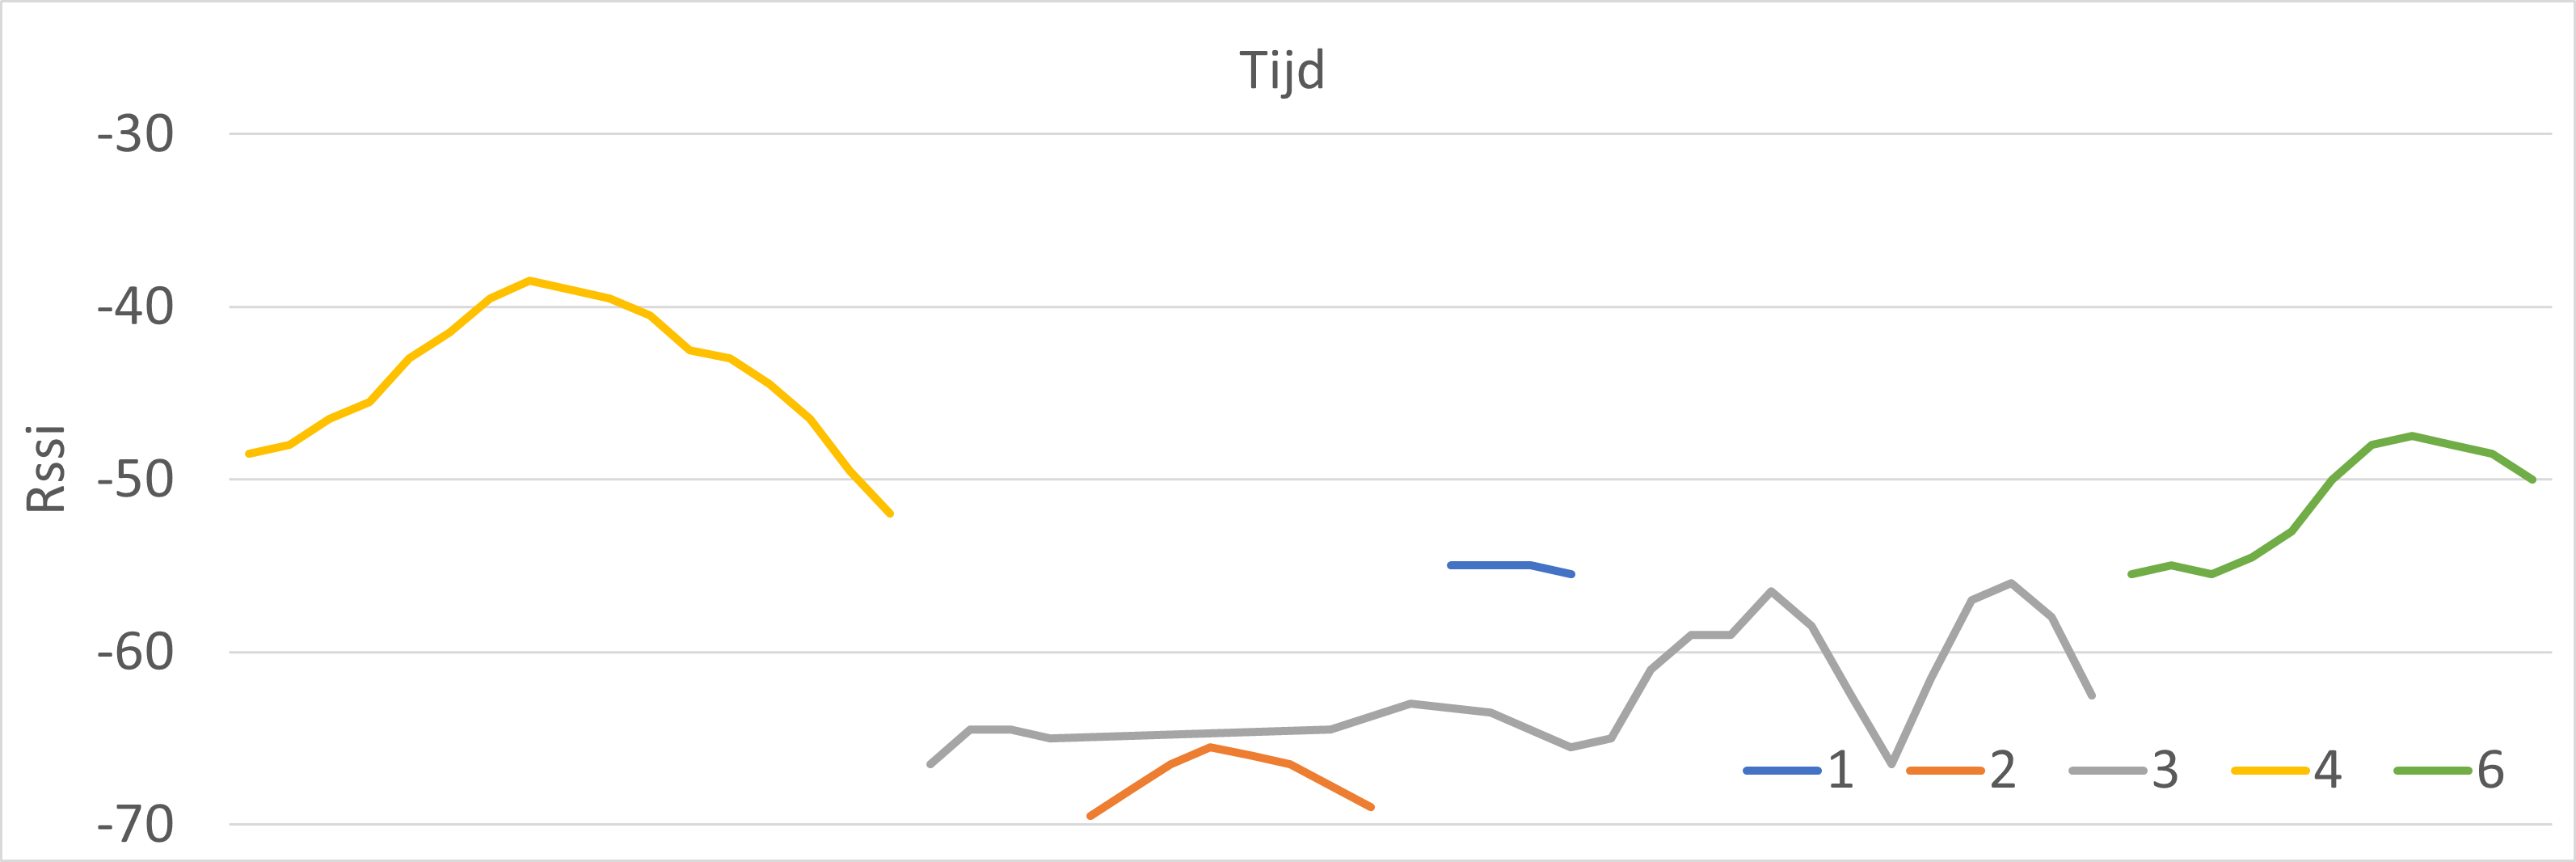
\includegraphics[width=\linewidth]{6b_RSSI}
	\caption{1 tag aan deurlijst - Testresultaat 2}
	\label{fig:ond-rfid-dynamic-6b-res}
\end{figure}

\paragraph{Testconclusie}
Als de asset tags niet meer op hetzelfde niveau liggen als de antenne, is hun detectie veel minder. Dit hoeft echter niet zo'n zeer probleem te zijn aangezien 1 meetpunt in theorie voldoende is om te weten dat het asset aanwezig is. Een tag die niet aanwezig is op de locatie zal uiteraard ook niet 1x antwoorden. Wel is het wegvallen van tags een probleem, want dan kan bijhorend asset niet gelokaliseerd worden, en deze kans wordt groter als de detectie verslecht.

\subsubsection{Deelconclusie}
Qua lokalisatie blijkt dit concept perfect te werken, echter is dit geen verrassing. Het voornaamste probleem is het kunnen detecteren van alle aanwezige tags, wat met een RFID opstelling niet vanzelfsprekend is. Hierdoor wordt de deelhypothese verworpen, aangezien deze niet waar is in een realistische situatie. Uiteraard is het mogelijk om met een andere hardwareopstelling een betere detectie te bekomen. Dit bv. met antennes op verschillende hoogtes, of een staafantenne met een ander detectieveld dan een vlakke antenne. Echter evolueert dit op deze manier in een RFID detectieprobleem en komt daarmee buiten de scope, nl. lokalisatie, van dit onderzoek te liggen. Verder is er binnen Aucxis voldoende ervaring op dit veld dat verder onderzoek in deze richting nutteloos is.

\section{BLE Vooronderzoek}
\label{sec:ond-ble-0}
Voordat overgegaan kan worden naar het onderzoeken van de opstellingen die gebruik maken van BLE, is het nodig enkele testen te doen om het gedrag van deze technologie vast te stellen, en om enkele veronderstellingen te testen.

\subsubsection{Test 1: Variatietest}
\label{sec:ond-ble-0-1}
De lokalisatieopstellingen verder in dit hoofdstuk zullen gebruik maken van RSSI waardes om de locatie van de beacons, en ook de bijhorende assets, te bepalen. Hierdoor is het belangrijk dat deze waardes constant zijn in de tijd als alle andere variabelen constant zijn. 
Voor deze test staan de gateway en de beacon op een afstand van 150cm uit elkaar, dit in hetzelfde vlak. Vervolgens wordt over lange tijd de RSSI waarde gemeten. Dit experiment wordt uitgevoerd bij 3 en bij 30 beaconberichten per gatewaybericht, dit om te bekijken of dit een effect heeft. Logischerwijs zal ook deze verhouding een invloed hebben, nl. hoe meer berichten de gateway heeft ontvangen, hoe meer de eventuele extreme waarden zullen worden uitgemiddeld. Door deze betere uitmiddeling zullen de waarden die de gateway uitstuurt stabieler worden.
De gebruikte beacons zijn 5 stuks van het type MokoSmart H5, en 2 van het type MokoSmart M2. Ze zijn allen aangeduid a.d.h.v. de laatste 2 karakters van hun MAC adres.

\paragraph{a) 3 beaconberichten per gatewaybericht}
Uit het testresultaat zichtbaar in grafiek~\ref{fig:ond-ble-1a-res} is duidelijk af te lijden dat een uitmiddeling van 3 berichten een zeer grote variatie veroorzaakt in de RSSI waarden. Met bij bv. beacon FB een verschil tussen de uitersten van 14 dBm. Aangezien de FSPL formule\footnote{Zie Sectie~\ref{sec:lit-definities} op pagina~\pageref{sec:lit-definities}} duidelijk maakt dat  een verschil van 6 dBm in theorie een verdubbeling van de afstand betekend, komt deze onzekerheid neer op een afstandsverschil van ongeveer factor 4. Het spreekt voor zich dat dit nefast is voor elke poging tot lokalisatie.

\begin{figure}[h]
	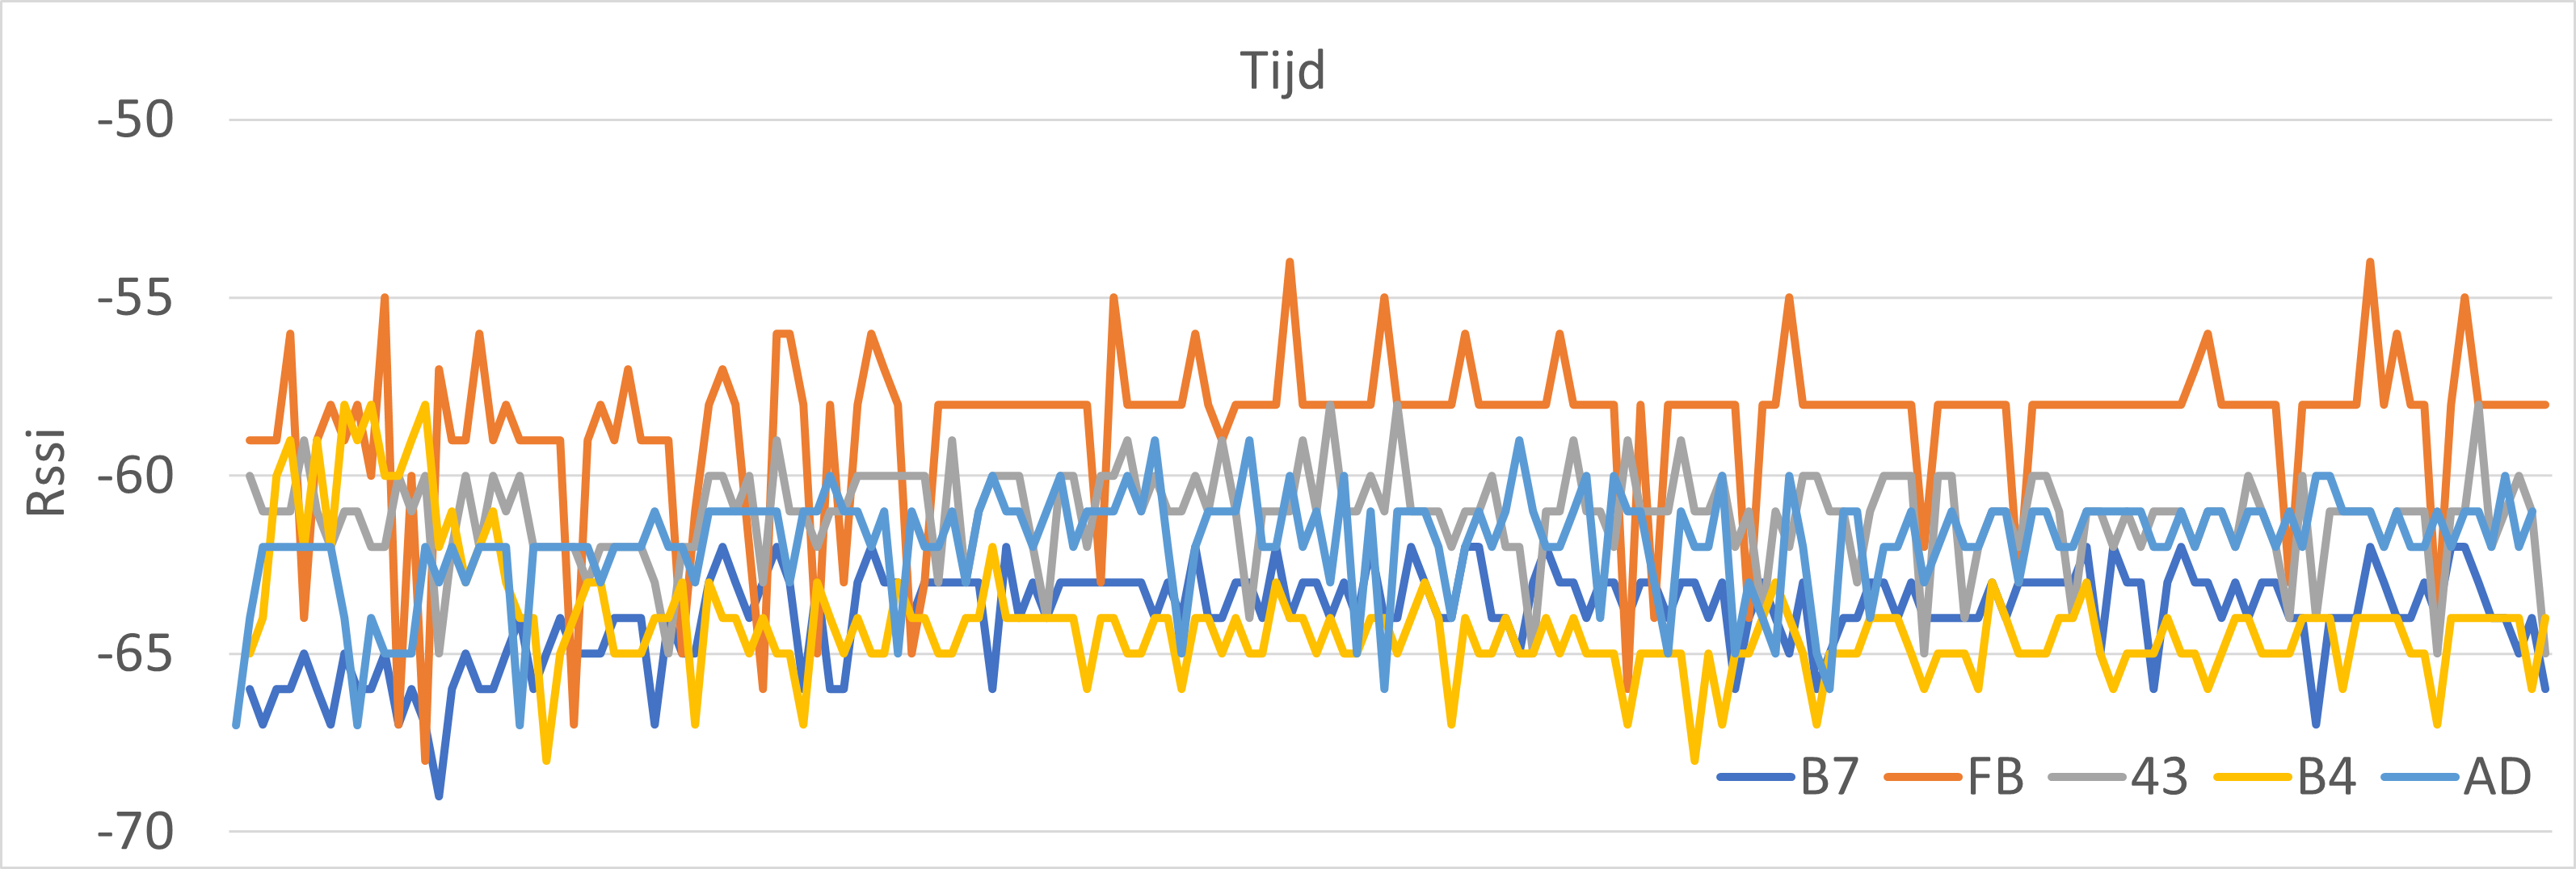
\includegraphics[width=\linewidth]{sble_0_1a}
	\caption{BLE Vooronderzoek - Testresultaat 1a}
	\label{fig:ond-ble-1a-res}
\end{figure}

\paragraph{b) 30 beaconberichten per gatewaybericht}
Uit deze test, met de resultaten weergegeven in grafiek~\ref{fig:ond-ble-1b-res}, is zichtbaar dat een uitmiddeling over 30 berichten veel minder variatie geeft. Dit met over het algemeen een variatie van plus en min 1 van de gemiddelde waarde. Dit lijkt meer acceptabel. Ook is er in dit experiment 1 H5 beacon (code AD) vervangen door 2 beacons van het type H2. Dit om een vermoeden te onderzoeken dat, alhoewel alle beacons dezelfde instellingen hebben, hun zendsterkte toch varieert. Dit is hier ook bevestigd, deze 2 (6F en 23) hebben een hogere gemiddelde RSSI waarde dan de 4 overgebleven H5 beacons. De H5 beacons onderling hebben echter ook een grote variatie.

\begin{figure}[h]
	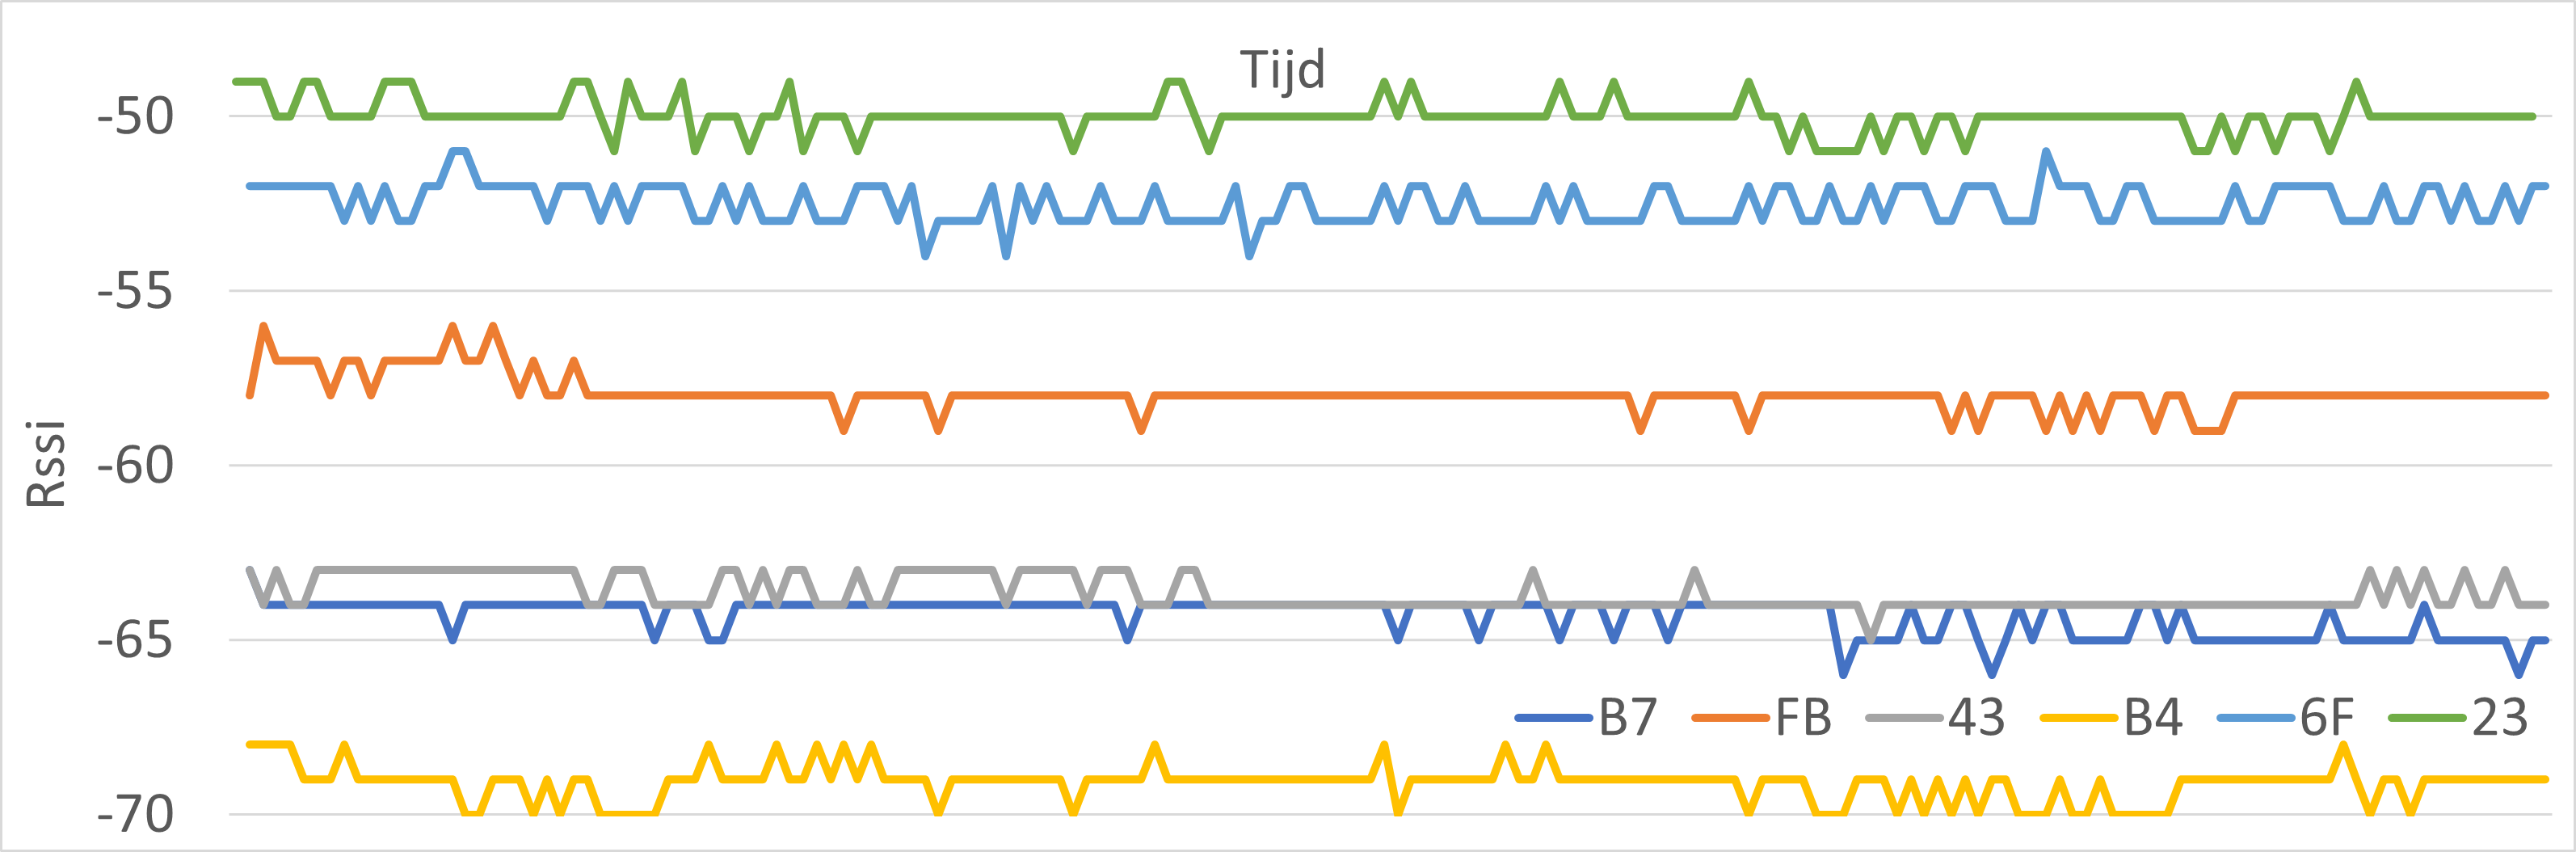
\includegraphics[width=\linewidth]{sble_0_1b}
	\caption{BLE Vooronderzoek - Testresultaat 1b}
	\label{fig:ond-ble-1b-res}
\end{figure}

\paragraph{Testconclusie}
Uit deze eerste test zijn 2 dingen duidelijk geworden, allereerst dat er een goed aantal beaconberichten nodig is voor uitmiddeling per gatewaybericht, anders zijn er grote variaties in de RSSI waarden. Aan het versnellen van de beacons is echter ook een groot nadeel verbonden, namelijk het verminderen van de batterijduur. Deze factor is rechtstreeks verbonden aan kostprijs, voor de nieuwe batterij, en de werkuren om deze te vervangen. Ook zal het afhangen van de use-case hoe belangrijk deze is. Alternatief kan ook de gateway trager uitsturen, wat een negatief effect zal hebben op de lokalisatiesnelheid. Dit zal een afweging zijn gebaseerd op de situatie maar is zeker niet onbelangrijk. Tijdens het verdere verloop van dit onderzoek zal een (arbitraire) waarde van 30 beaconberichten per gatewaybericht worden aangehouden, aangezien dit een mooie middenweg lijkt, maar dit kan verhoogd of verlaagd worden met de voor- en nadelen vandien.

Als 2e is er ook duidelijk geworden dat er een verschil zit tussen de zendsterkte van BLE beacons met dezelfde instellingen. Dit zowel voor beacons van hetzelfde type, als van andere types. Hieruit volgt dat, als er een omzetting van RSSI waarde naar een afstand moet worden gemaakt, deze waarde op een of andere manier zal moeten worden genormaliseerd. Een mogelijkheid hiervoor is het veld 'RSSI at 0m', aanwezig in een UID bericht\footnote{Zie 'Het Eddystone protocol' in Sectie~\ref{subsec:lit-ble} op pagina~\pageref{subsec:lit-ble}}. Een andere optie is de beacons kalibreren dat ze even sterk zenden. Ongeacht hoe hier rond wordt gewerkt, blijft het een aandachtspunt.

\subsubsection{Test 2: Afstandstest}
\label{sec:ond-ble-0-2}
De volgende veronderstelling die zal worden getest, is het verloop van de RSSI waardes, in functie van afstand tussen de beacons en de gateway. In theorie zou deze moeten verlopen volgens de FSPL formule\footnote{Zie Sectie~\ref{sec:lit-definities} op pagina~\pageref{sec:lit-definities}} (logaritmisch, met en neerwaarts traject van ~6dBm per verdubbeling van de afstand). Deze test heeft als doel na te gaan of dit in praktijk ook zo is.
Voor dit experiment is een gateway op een tafel geplaatst, verder is er een beacon die steeds verder van deze gateway zal verwijderd worden in intervallen van 50cm. Dit experiment zal 3x worden herhaald, 1x in een ideale omgeving, nl. een anechoïsche kamer\footnote{Een anechoïsche kamer is een kamer waarvan de muren bedekt zijn met speciaal gevormd mousse, meestal puntvormig. Dit is bedoeld om radio- en geluidsgolven zo goed mogelijk te absorberen en zo een kamer te creëren met zo weinig mogelijk reflecties.}. 1x in een open reële omgeving, nl. een bemeubelde huiskamer. En als laatste ditzelfde nogmaals, maar met 1 muur tussen, om zo het verwachte negatieve effect van obstakels te controleren. De meting in ideaal geval zal minder meetpunten bevatten dan de reële, omwille van de gelimiteerde grootte van de anechoïsche kamer.

\subsubsection{Resultaat}
Uit het testresultaat zichtbaar in grafiek~\ref{fig:ond-ble-2-res} is duidelijk zichtbaar dat theorie en realiteit veel van elkaar verschillen. De (beperkte) meetpunten van de ideale meting komen zeer goed in de buurt van de theorie, maar vanaf er wordt overgestapt naar een open reële ruimte zijn de resultaten zeer anders. Met als voornaamste bevindingen dat de waarden veel lager liggen dan in theorie, en dat het verloop niet in alle gevallen dalend is. Wel is aan de bijgetekende logaritmische trendlijn te zijn dat de reële waarden wel een dalend verloop hebben. Op de meting met muur is verder ook een grillig, maar neerwaarts verloop zichtbaar, dit keer op een lager niveau dan zonder muur.

\begin{figure}[h]
	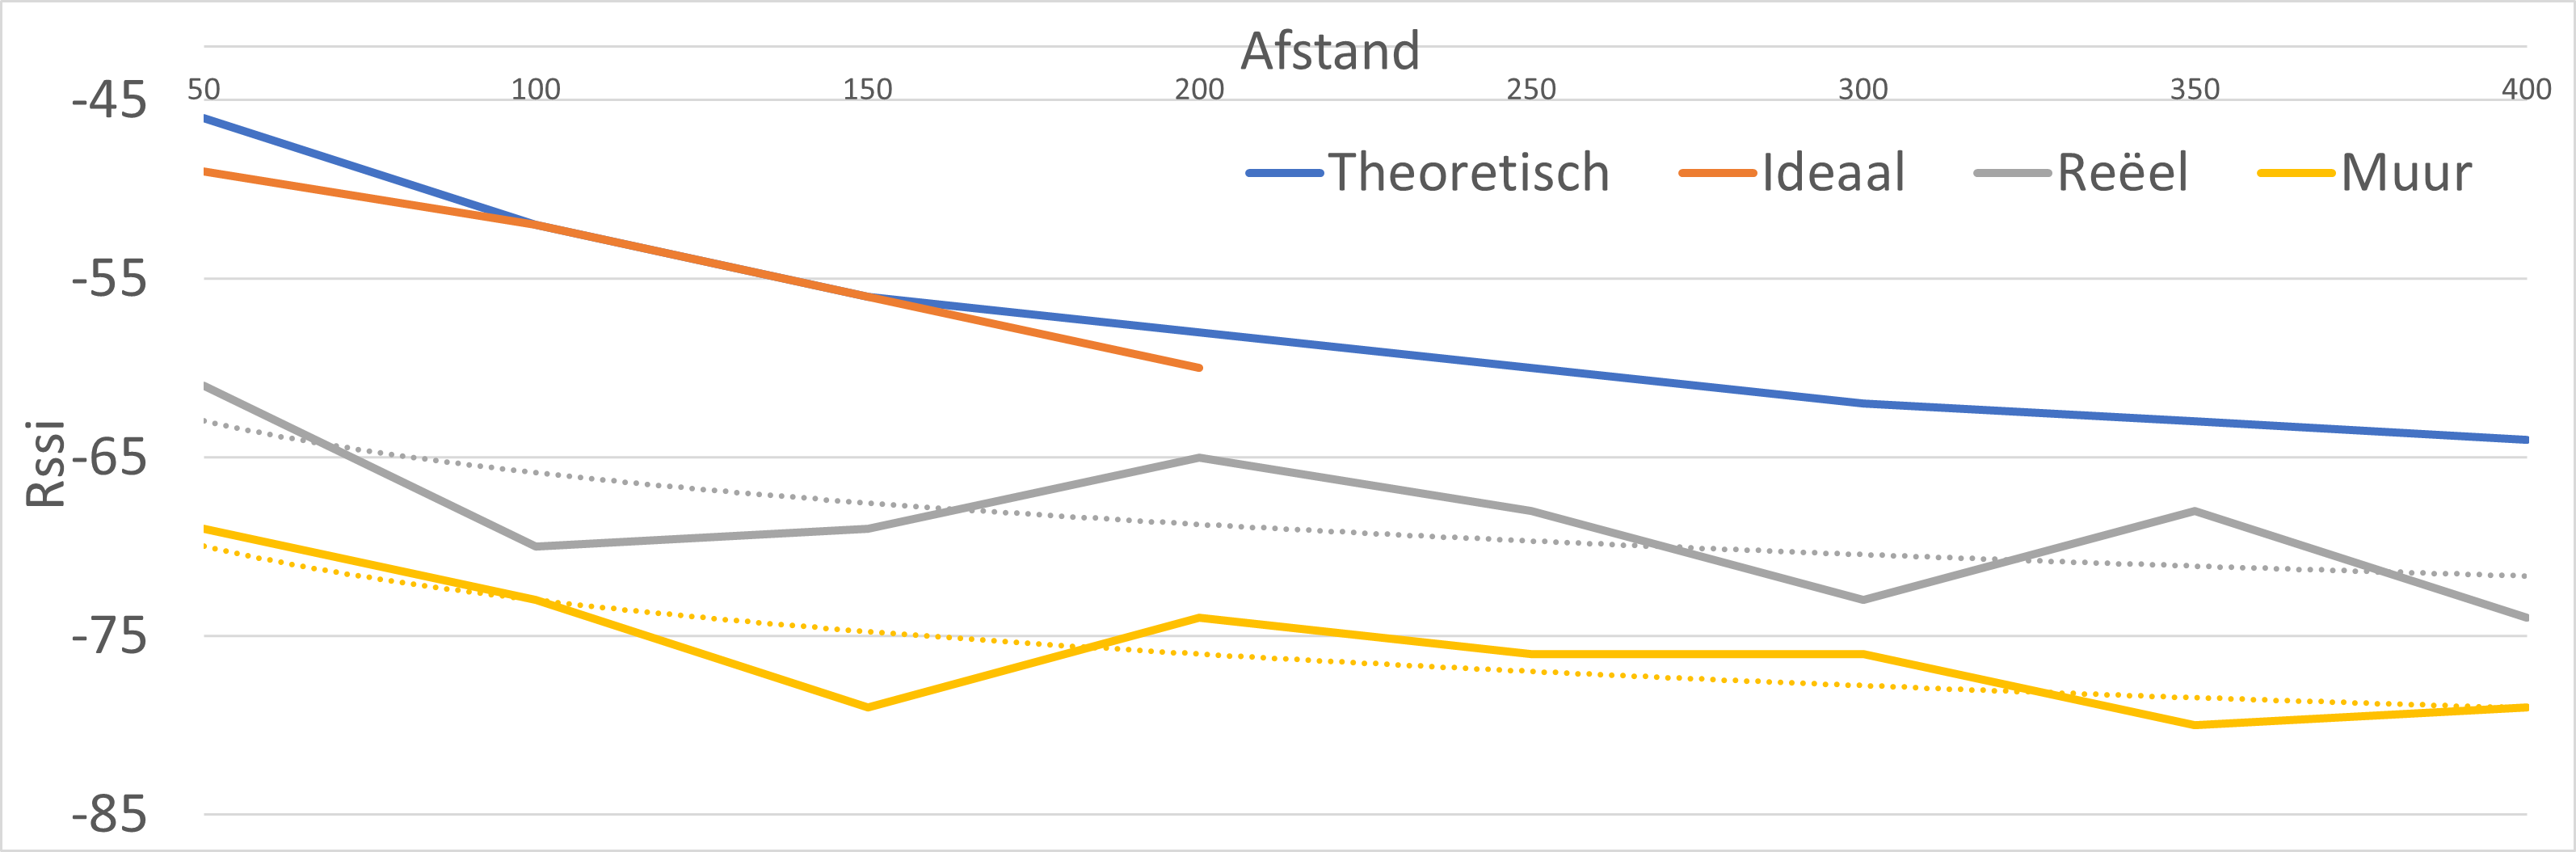
\includegraphics[width=\linewidth]{sble_0_2}
	\caption{BLE Vooronderzoek - Testresultaat 2}
	\label{fig:ond-ble-2-res}
\end{figure}

\emph{De reële testen zijn uitgevoerd met 5 verschillende MokoSmart H5 beacons, echter aangezien allen een gelijkaardig verloop vertoonden, worden de andere 4 niet extra bijgevoegd.}

\paragraph{Testconclusie}
Aangezien het voornaamste verschil tussen de ideale en realistische situatie het bestaan van reflecties is, is met deze test duidelijk geworden dat deze een zeer grote impact hebben op de RSSI waarden. Voornamelijk in de vorm van een schommeling, welke vervelend is als er een conversie moet worden gemaakt tussen RSSI en afstand, en verder ook in een algehele RSSI vermindering tegenover de theorie. 
De testen voor de effectieve scenario's zullen allen plaatsvinden in reële omgevingen, aangezien implementaties van systemen gebaseerd op deze scenario's ook in reële ruimtes zullen werken, en puur theoretische of ideale situaties geen nut hebben om te vergelijken.

\subsubsection{Test 3: Rotatietest}
\label{sec:ond-ble-0-3}
Deze derde en laatste test in dit vooronderzoek zal de veronderstelling testen dat de meting van de gateway richtingsonafhankelijk is. Anders gezegd zal deze test onderzoeken of er een verschil is in RSSI als de enige variabele de locatie van de beacon rond de gateway is.
Voor deze test is een gateway opgesteld op een draaiplatform in een anechoïsche kamer, met een MokoSmart H5 beacon op 150cm afstand. Tijdens de test draait de gateway rond zijn as. Dit gebeurt 2x, eens met de beacon op dezelfde hoogte als de gateway, en eens met de beacon 50cm hoger.

\paragraph{a) Beacon en gateway op zelfde hoogte}
\begin{minipage}{0.55\textwidth}
Uit dit resultaat, zichtbaar in grafiek~\ref{fig:ond-ble-3a-res}, is duidelijk dat er een zekere richtingsafhankelijk is. Er is een grote blindspot rond 260° van -68 dBm, een verschil met het gemiddelde\footnotemark van 10dBm. Verder zijn er ook 2 kleinere op 80° en 180° met een verschil van 5 dBm. Alhoewel niet drastisch, het overgrote deel van is vrij constant, is dit toch noemenswaardig. De meest voor de hand liggende verklaring hiervoor is het feit dat de ingebouwde staafantenne loopt op de lijn van 90° en 270°. De 2 voornaamste dippen wijzen ongeveer naar de uiteinden van deze antenne, en een blindspot hier is karakteristiek voor een staafantenne.
\end{minipage}
\footnotetext{Aangegeven op de figuur met een oranje stippellijn}
\hfill
\begin{minipage}{0.42\textwidth}
	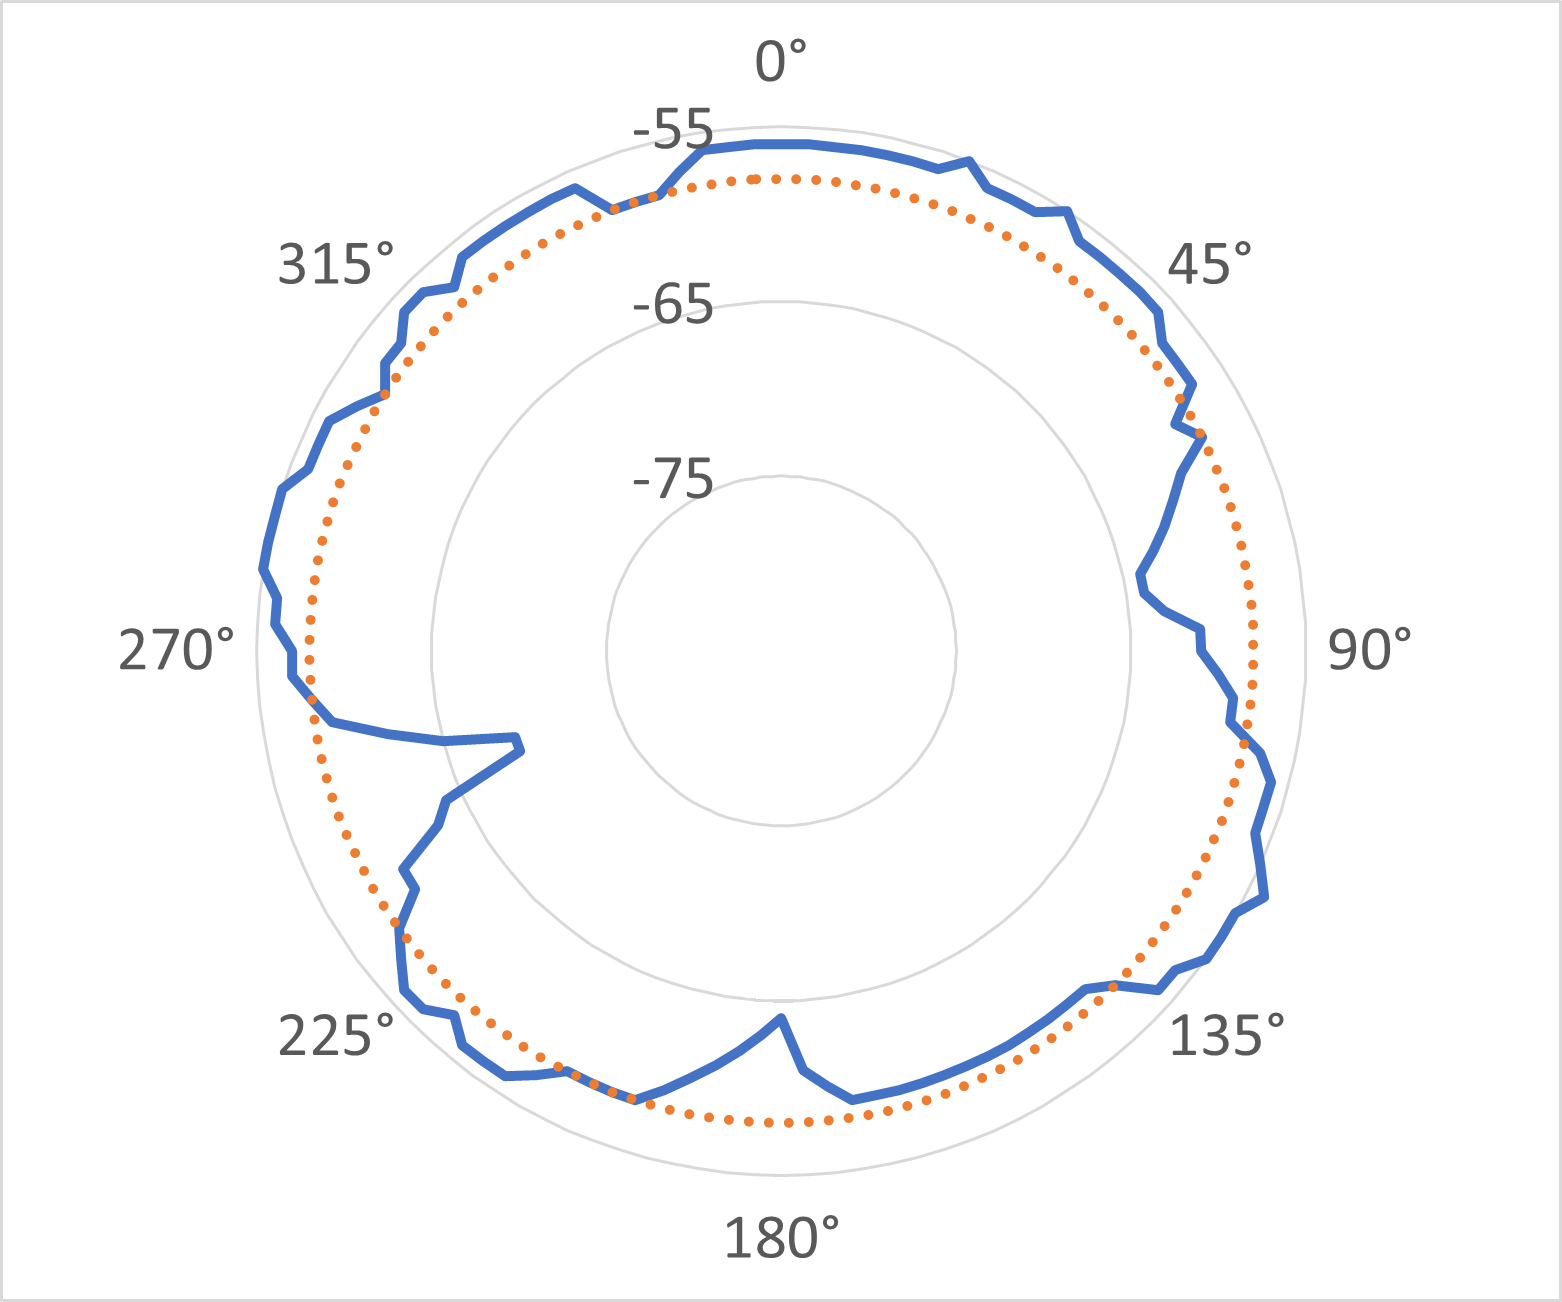
\includegraphics[width=\linewidth]{sble_0_3a}
	\captionof{figure}{BLE Vooronderzoek - Testresultaat 3a}
	\label{fig:ond-ble-3a-res}
\end{minipage}


\paragraph{b) Beacon 50cm boven gateway}
\begin{minipage}{0.55\textwidth}
In grafiek~\ref{fig:ond-ble-3b-res} is zichtbaar dat de harde blindspots uit de vorige test verdwenen zijn, wat het vermoeden dat dit met de antennerichting te maken heeft lijkt te bevestigen. Wel is er nog een duidelijk dal in het kwartaal tussen 225° en 315°.
\end{minipage}
\hfill
\begin{minipage}{0.42\textwidth}
	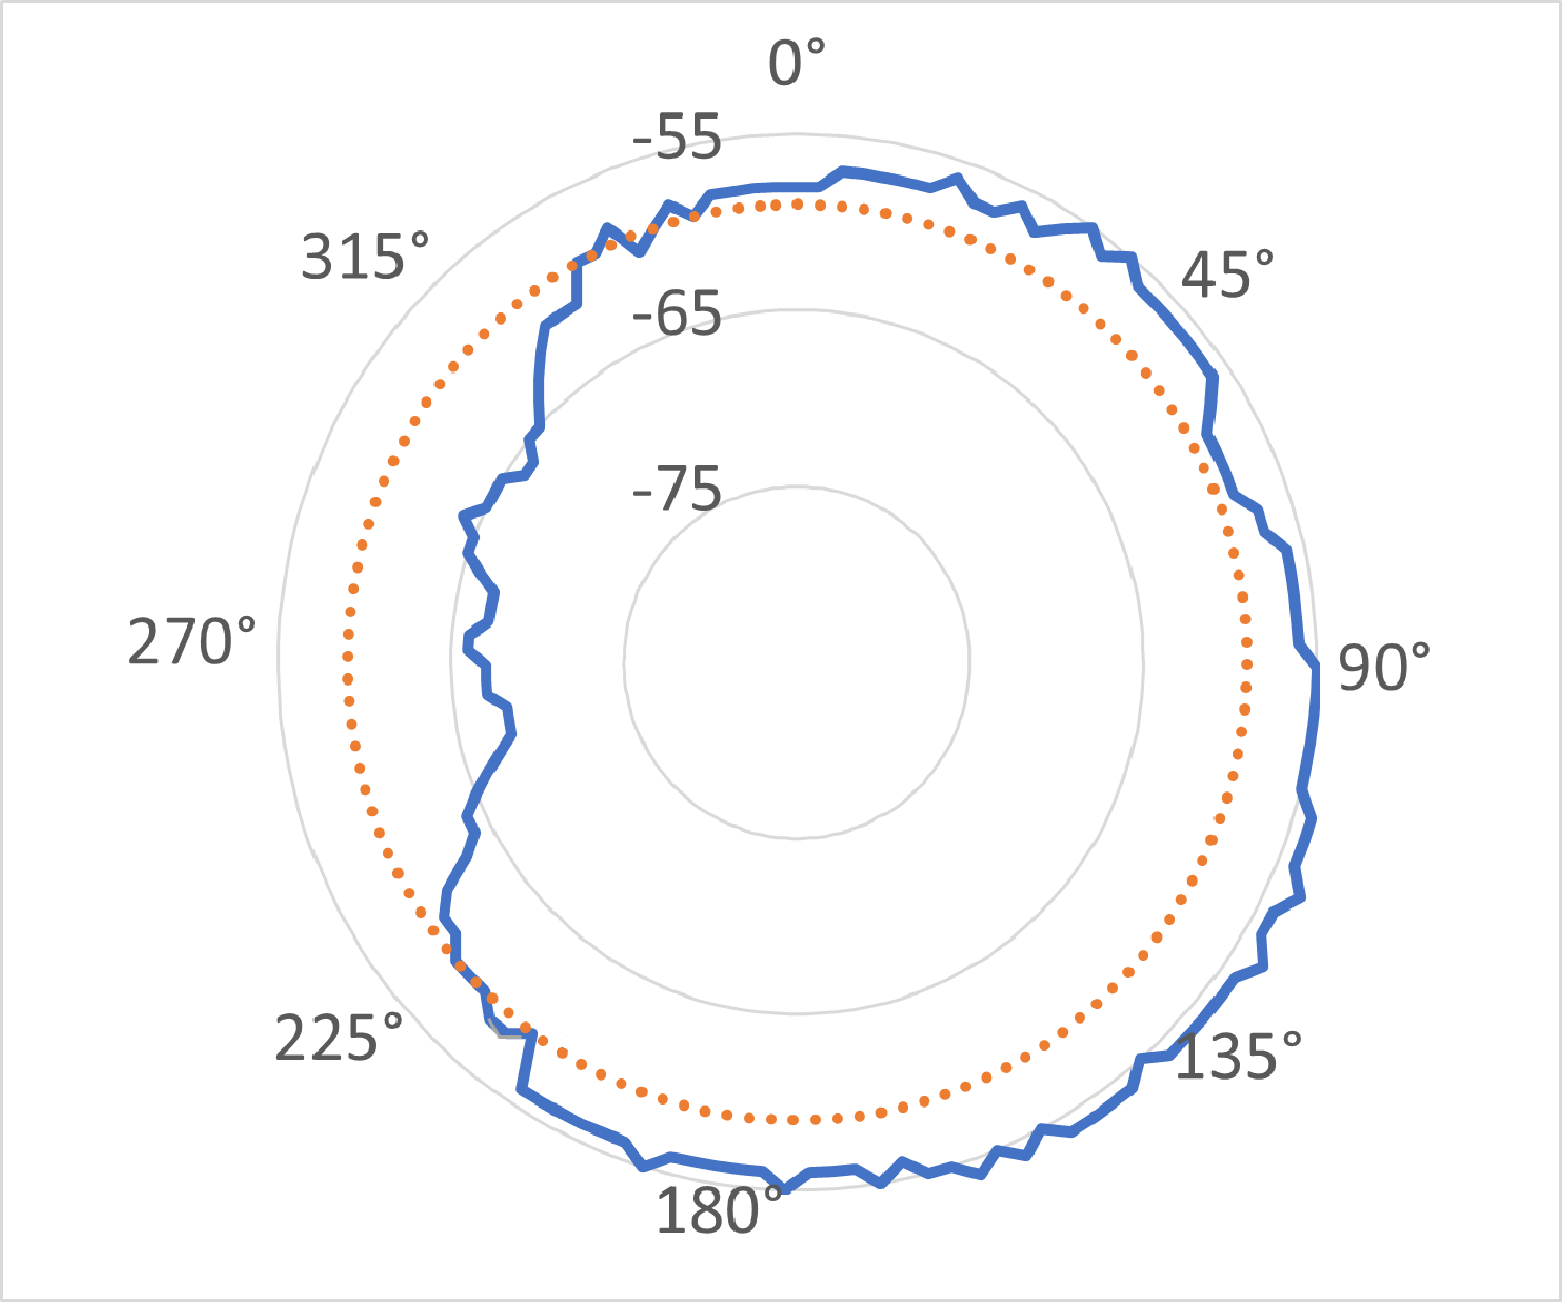
\includegraphics[width=\linewidth]{sble_0_3b}
	\captionof{figure}{BLE Vooronderzoek - Testresultaat 3b}
	\label{fig:ond-ble-3b-res}
\end{minipage}

\paragraph{Testconclusie}
Uit deze test is duidelijk geworden dat een gateway niet 100\% richtingsonafhankelijk is. Over de grote lijn zal dit vermoedelijk geen problemen geven, echter kunnen de plotse daten in meetgevoeligheid onverwachte waarden opleveren als een beacon toevallig net in die richting ligt.
Tijdens de volgende testen zullen alle gateways in dezelfde richting worden geplaatst om het effect van deze verlopen te standaardiseren. 

\subsubsection{Deelconclusie}
Uit dit vooronderzoek is duidelijk geworden dat niet elke theoretische veronderstelling ook geldig is in praktijk. Het is belangrijk dit eerst vastgesteld te hebben, aangezien het waarschijnlijk mogelijk zal zijn om sommige anders onverklaarbare fenomenen in komende scenariotests te verklaren. Ook zijn er in de testconclusies maatregelen/standaarden vastgelegd om deze effecten zo veel mogelijk te standaardiseren.

\section{Statische BLE}
\subsection{1 gateway per locatie}
\label{sec:ond-ble-1}

\subsubsection{Deelhypothese}
Deze opstelling is in staat om verspreide, getagde assets te detecteren en eenduidig een locatie toe te wijzen.

\subsubsection{Test 1: 6 locaties in reële, open ruimte, gelijk verdeeld}
\label{sec:ond-ble-1-1}
\begin{minipage}{0.55\textwidth}
De eerste test voor deze opstelling is een best case opstelling, welke zichtbaar is in figuur~\ref{fig:ond-ble-static-1-1-ops}. In een open ruimte staan 6 gateways\footnotemark in een raster, op een afstand van 2m van elkaar. Vervolgens is de ruimte in 6 even grote locaties verdeeld, met elk 1 gateway in het midden van deze locaties. In praktijk komt deze locatieafscheiding\footnotemark neer op een raster middendoor de gateways. Verder liggen er verschillende MokoSmart H5 en M2 beacons verdeeld over de ruimte\footnotemark, en zal worden bekeken waar zij volgens de gemeten waarden zich bevinden. Hierna volgt een vergelijking met hun echte positie.
\end{minipage}
\footnotetext[9]{Gateways worden aangeduid door een grijs blokje met een bijhorende letter. De illustraties zijn ook voorzien van 2 rode stippen op de gateway, deze illustreren de voorkant (0°) van de gateway.}
\footnotetext[10]{De grenzen van locaties worden in de illustraties weergegeven door een stippellijn.}
\footnotetext{Beacons worden aangeduid in de illustraties door een cijfer.}
\hfill
\begin{minipage}{0.42\textwidth}
	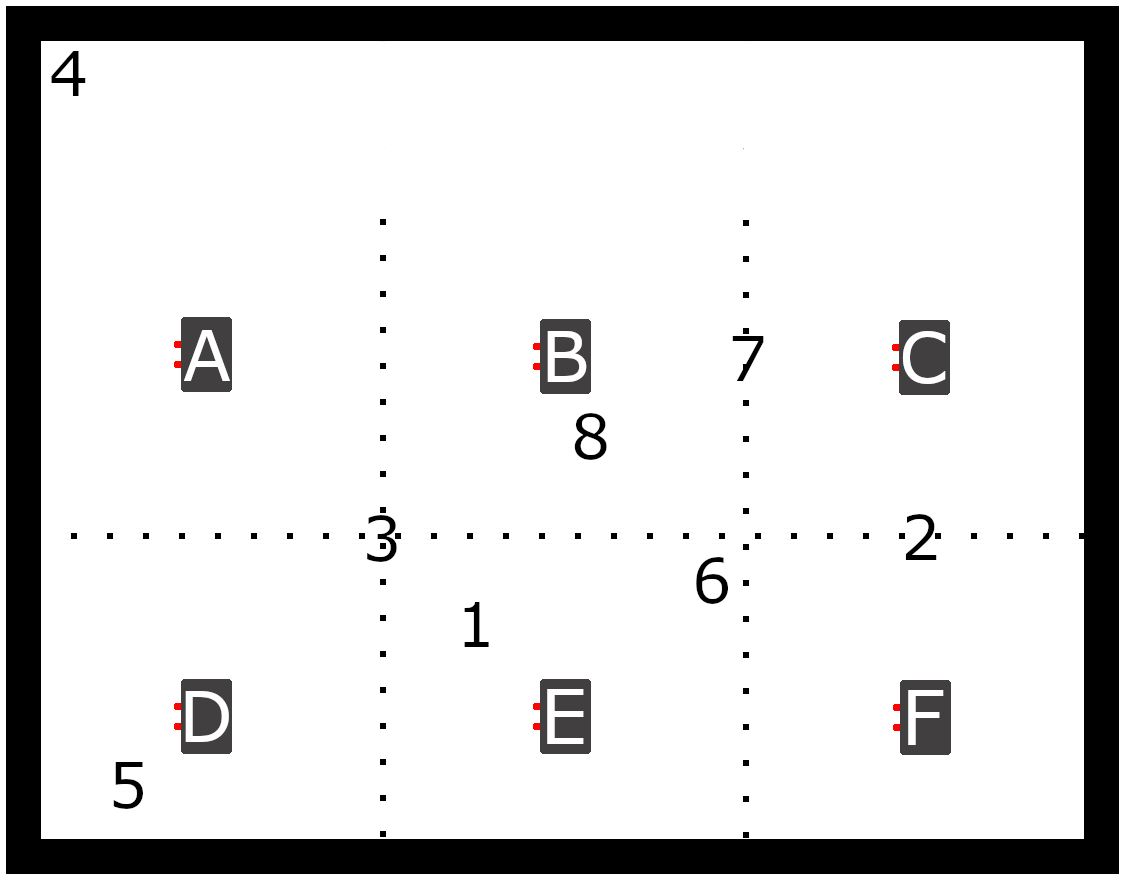
\includegraphics[width=\linewidth]{sble_1_1_floor}
	\captionof{figure}{1 gateway per locatie - Opstelling 1}
	\label{fig:ond-ble-static-1-1-ops}
\end{minipage}

\paragraph{Resultaat}
\begin{minipage}{0.55\textwidth}
De resultaten van deze test zijn zichtbaar in tabel~\ref{fig:ond-ble-static-1-1-res}. De hoogste RSSI waarde is karakteristiek voor de kortste afstand tot een gateway, en wordt gebruikt om de locatietoewijzingen te doen. Deze hoogste waarden staan aangeduid in het groen. Een toewijzing op deze manier verloopt op het eerste zicht vrij goed. Ook beacons op de grenslijn zijn toegewezen aan 1 van hun aangrenzende locaties. Enkel bij beacon 6 en 8 is een verschil te vinden.
\end{minipage}
\hfill
\begin{minipage}{0.42\textwidth}
	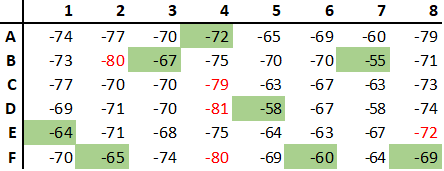
\includegraphics[width=\linewidth]{sble_1_1_results}
	\captionof{table}{1 gateway per locatie - Testresultaat 1}
	\label{fig:ond-ble-static-1-1-res}
\end{minipage}

Er bestaat een onderscheid in soorten beacons, en die horen apart besproken te worden. Dit in volgorde van moeilijkheid. Allereerst zijn er de beacons die duidelijk in een locatie liggen, en buiten het raster van gateways. Tijdens deze test zijn dit beacon 4 en 5. Deze zijn beiden met een comfortabel RSSI verschil gecategoriseerd in de juiste locatie. Verder zijn er de beacons die zich duidelijk binnen een locatie bevinden, maar binnen het raster van gateways. Bij deze test zijn dit beacons 1 en 8. Hoewel beacon 1 met voorsprong correct is, is er iets vreemd gebeurd bij beacon 8. Deze staat gecategoriseerd bij gateway F, en deze vertegenwoordigt een niet aangrenzende locatie.  Dit is zeer vreemd aangezien deze zeer dicht bij gateway B lag. Een mogelijke verklaring ligt bij het stralingspatroon van de gateway, waaruit blijkt dat deze beacon in een blindspot ligt\footnote{Zie 'Test 3: Rotatietest' in sectie~\ref{sec:ond-ble-0} op pagina~\pageref{sec:ond-ble-0}}. Verder zijn er de grensgeval beacons, waaronder beacon 2 en 7, welke op de grens tussen 2 locaties liggen. Zij zijn echter toegewezen aan 1 van deze 2, welke in orde is, aangezien het in dit scenario niet de bedoeling is om een exacte positie te bepalen, maar toewijzing aan een locatie te doen. En als laatste beacon 3 en 6 op een 4-punt. Beacon 3 is ook aangrenzend toegewezen ook in orde. Beacon 6, alhoewel fysiek net over de grens van locatie E liggend, is toegewezen aan aangrenzende locatie F. In theorie is dit een fout, maar geen grote. Ook is een zekere foutmarge bij de locatiegrenzen geen verassing, gezien de onzekerheden in de RSSI waarden vastgesteld in het vooronderzoek\footnote{Zie 'Test 2: Afstandstest' in sectie~\ref{sec:ond-ble-0} op pagina~\pageref{sec:ond-ble-0}}.

\paragraph{Testconclusie}
De eerste test heeft bewezen dat dit lokalisatiescenario mogelijkheden heeft, op zijn minst in een eenvoudige egale opstelling. 1/8 zeer fout gelokaliseerde assets is niet perfect maar ook niet zeer slecht.

\subsubsection{Test 2: 6 even grootte in reële, open ruimte, ongelijk verdeeld}
\label{sec:ond-ble-1-2}
\begin{minipage}{0.55\textwidth}
Voor deze test veranderen de locaties van gelijke grootte uit vorige test in locaties van variabele grootte en vorm, zoals zichtbaar in figuur~\ref{fig:ond-ble-static-1-3-ops}. Verder is de ruimte, hoewel nog steeds open, niet meet convex. De locaties blijven dit wel. Hier is het niet zo dat elk punt zich ook bij zijn dichtstbijzijnde gateway bevind qua locatie. 
\end{minipage}
\hfill
\begin{minipage}{0.42\textwidth}
	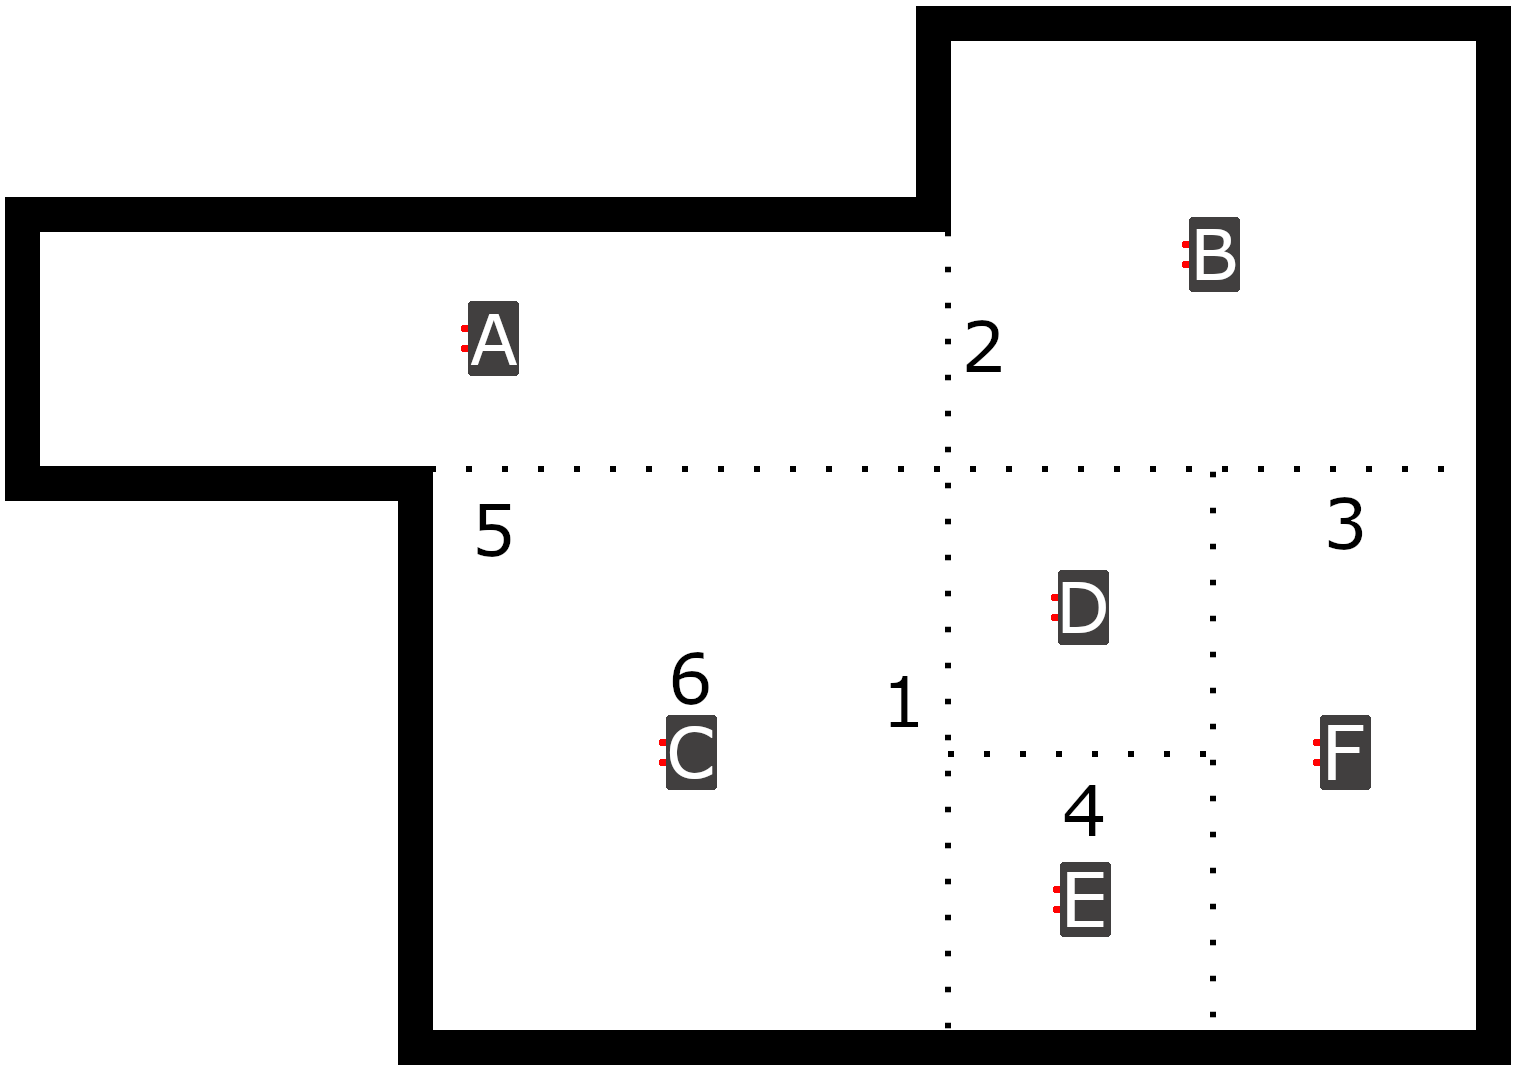
\includegraphics[width=\linewidth]{sble_1_3_floor}
	\captionof{figure}{1 gateway per locatie - Opstelling 2}
	\label{fig:ond-ble-static-1-3-ops}
\end{minipage}

\paragraph{Resultaat}
\begin{minipage}{0.55\textwidth}
De resultaten van deze test zijn zichtbaar in tabel~\ref{fig:ond-ble-static-1-3-res}. Van de 6 beacons zijn er 3 correct en 3 fout toegewezen. Echter zijn de 3 fout toegewezen beacons (1, 3 en 5) de beacons die dichter lagen bij de toegewezen locatie gateway dan bij de theoretisch correcte locatie gateway. De andere 3 beacons (2, 4 en 6) zijn wel correct toegewezen. 
\end{minipage}
\hfill
\begin{minipage}{0.42\textwidth}
	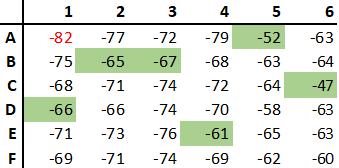
\includegraphics[width=\linewidth]{sble_1_3_results}
		\captionof{table}{1 gateway per locatie - Testresultaat 2}
	\label{fig:ond-ble-static-1-3-res}
\end{minipage}

\paragraph{Testconclusie}
Deze test bevestigd het vermoeden dat deze lokalisatie strategie het slechter zal doen bij locaties van verschillende groottes, door de de basering op hoogste RSSI en de link met de afstand. Dit zeker in een open ruimte waar deze afstand de enige bepalende factor voor de RSSI is (uiteraard buiten de onzekerheden vastgesteld tijdens het BLE vooronderzoek). Een mogelijke remedie hiervoor is een RSSI filter te plaatsen op gateways voor kleinere locaties. Dit zodat het gebied dat ze stelen van aanpalende grotere ruimtes verkleind. Echter omdat het bereik nog steeds (theoretisch) een cirkel blijft zullen vreemde verschijnsels bij locatieovergangen onvermijdelijk blijven.

\subsubsection{Test 3: 5 realistische locaties}
\label{sec:ond-ble-1-3}
\begin{minipage}{0.55\textwidth}
Deze derde een laatste test van deze opstelling vergroot het concept van vorige test en voegt muren toe zodat de opstelling realistischer wordt. Dit is zichtbaar in figuur~\ref{fig:ond-ble-static-1-4-ops}. Deze opstelling bestaat uit 5 locaties, ondergebracht in 5 ruimtes van verschillende groottes, gescheiden door muren. Daardoor is de afstand niet meer de enige bepalende factor voor de RSSI waarde, maar ook tussenliggende muren. Dit kan in theorie een groter verschil geven, en kan het grootteverschil tussen locaties wat compenseren. Dit experiment zal ook 2x worden uitgevoerd, 1x met tussenliggende deuren gesloten, en 1x open. Dit om ook het mogelijke effect van deuren te onderzoeken.
\end{minipage}
\hfill
\begin{minipage}{0.42\textwidth}
	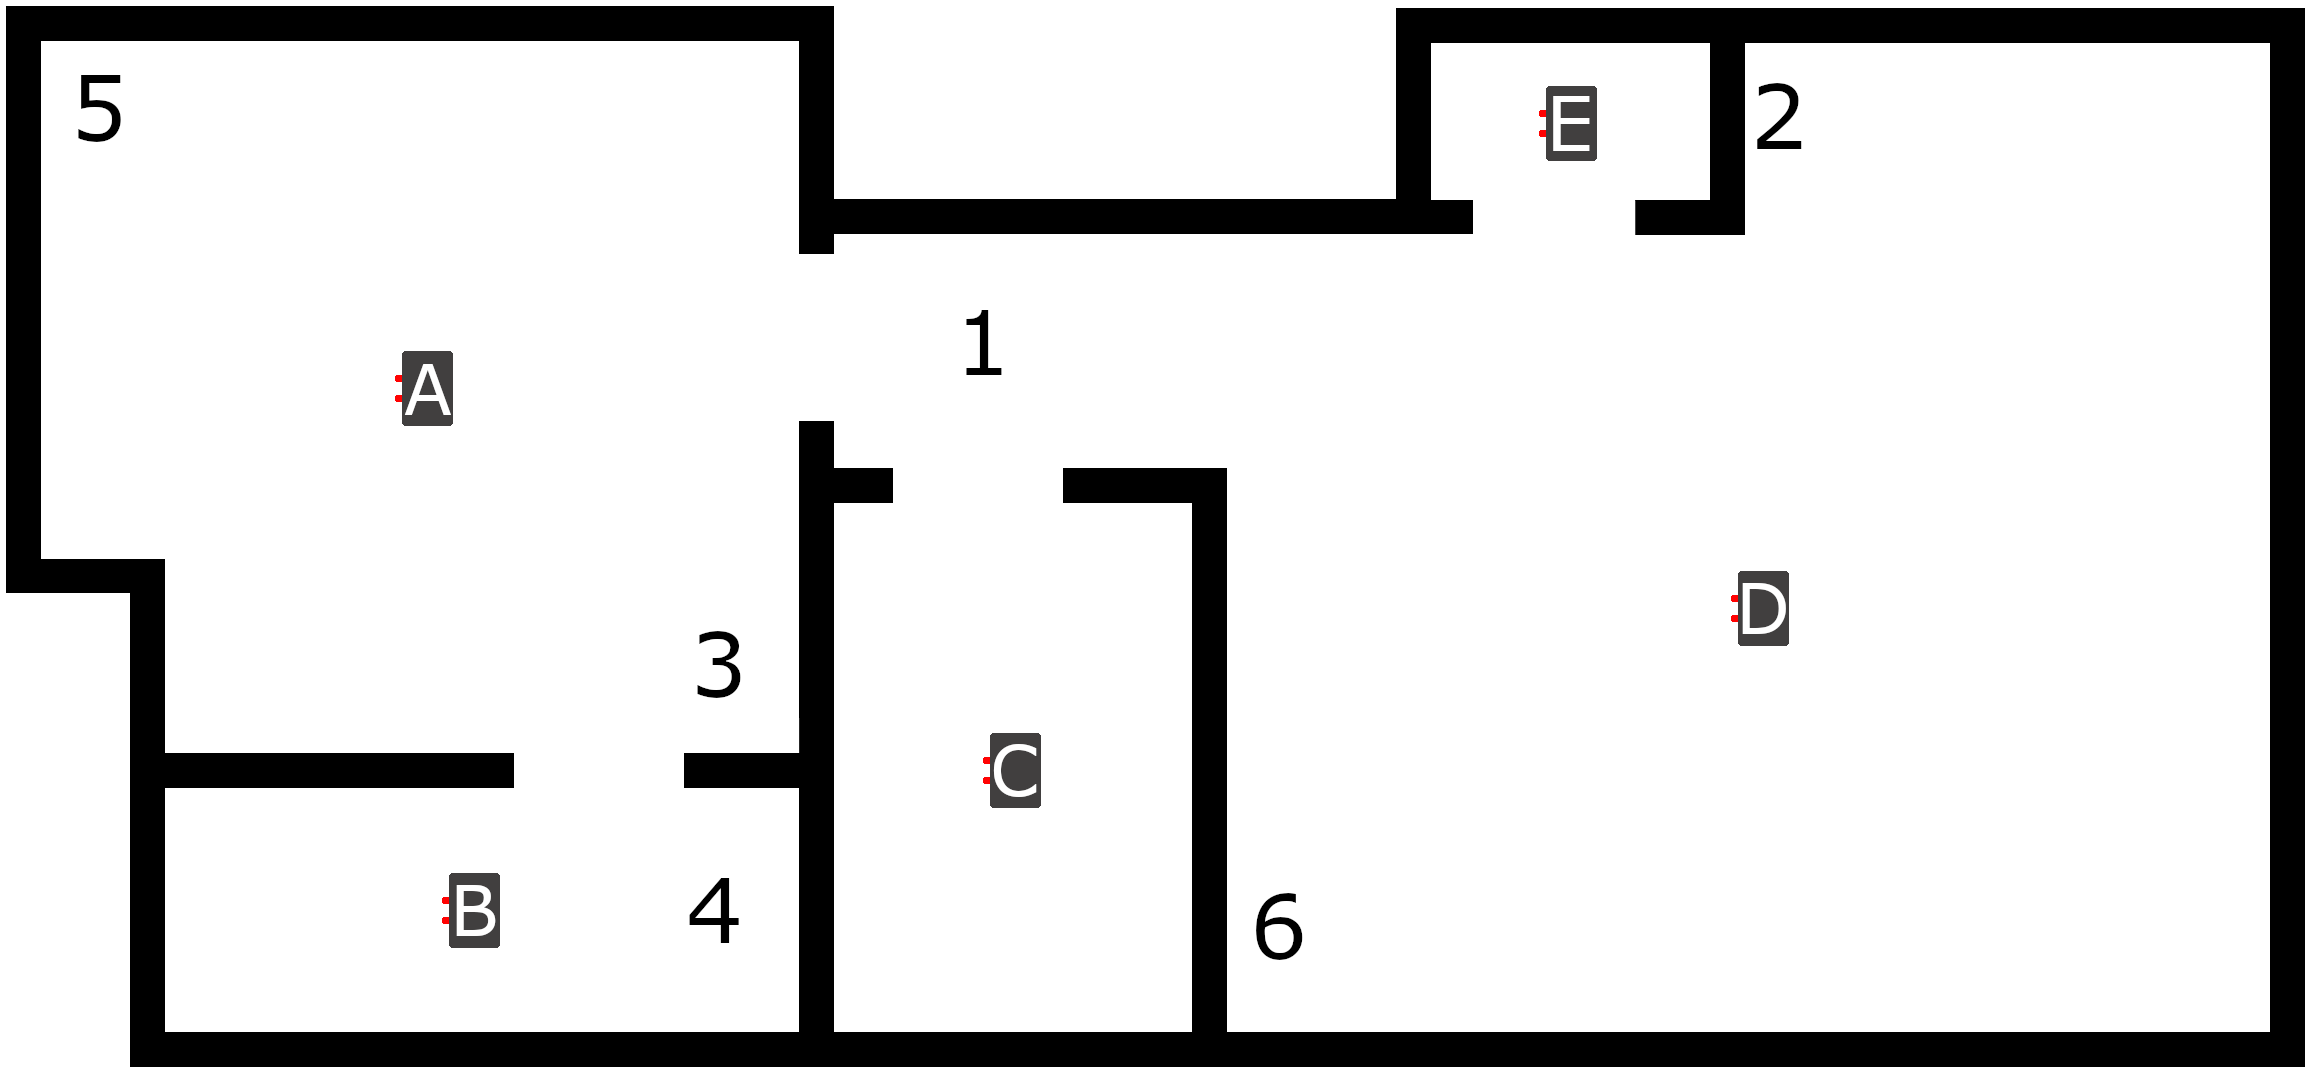
\includegraphics[width=\linewidth]{sble_1_4_floor}
	\captionof{figure}{1 gateway per locatie - Opstelling 3}
	\label{fig:ond-ble-static-1-4-ops}
\end{minipage}

\paragraph{a) Deuren gesloten}
\begin{minipage}{0.55\textwidth}
Uit de resultaten in tabel~\ref{fig:ond-ble-static-1-4a-res} is af te leiden dat dit principe zeer goed werkt, met een perfecte lokalisatie. Dit is geen verassing voor de duidelijke, safe beacons (4 en 5). De andere 4 beacons liggen echter stuk voor stuk dichter bij de gateway van een andere locatie dan bij die van zichzelf, met een muur tussen. In het bijzonder is er beacon 2, welke op ongeveer 50cm ligt van gateway E, en op 250cm van gateway D. Toch wordt deze nog steeds correct bij locatie D gecategoriseerd.
\end{minipage}
\hfill
\begin{minipage}{0.42\textwidth}
	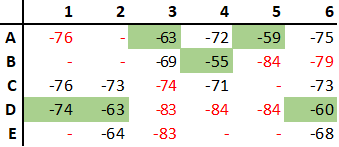
\includegraphics[width=\linewidth]{sble_1_4a_results}
	\captionof{table}{1 gateway per locatie - Testresultaat 3a}
	\label{fig:ond-ble-static-1-4a-res}
\end{minipage}

\paragraph{b) Deuren open}
\begin{minipage}{0.55\textwidth}
Deze resultaten, weergegeven in tabel~\ref{fig:ond-ble-static-1-4b-res}, tonen geen noemenswaardig verschil met de test met gesloten deuren. Alles blijft correct gecategoriseerd, maar ook de waardes verschillen niet veel. Dit is vooral verrassend bij beacon 1, welke met open deur rechtstreeks zichtbaar is voor gateway A, maar toch correct bij gateway D blijft ingedeeld.
\end{minipage}
\hfill
\begin{minipage}{0.42\textwidth}
	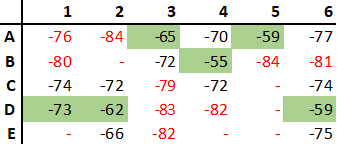
\includegraphics[width=\linewidth]{sble_1_4b_results}
	\captionof{table}{1 gateway per locatie - Testresultaat 3b}
	\label{fig:ond-ble-static-1-4b-res}
\end{minipage}

\paragraph{Testconclusie}
Deze test toont mooi aan dat de extra isolatie van een muur een zeer positieve invloed heeft op een lokalisatie volgens dit principe. Verder toont ze ook aan dat een verschil in grote tussen aanpalende ruimtes niet noodzakelijk een groot probleem hoeft te zijn. Uiteraard zal ook het soort muur een invloed hebben op deze resultaten. In de testopstelling worden muren uit cellenbeton gebruikt, maar een dunnere muur uit bv. kalkplaat zal mogelijk een minder isolerend effect hebben. Ook is duidelijk dat een deur weinig impact heeft op de resultaten. Ook dit kan natuurlijk aan het materiaal liggen. Een houten deur zoals in de testopstelling is klaarblijkelijk verwaarloosbaar, maar bv. een nooddeur, speciaal als er metaal in zit, zal een grotere impact hebben.

\subsubsection{Deelconclusie}
Al bij al is dit een zeer acceptabel scenario, het merendeel van de lokalisaties was geslaagd. Dit met uitzondering van fouten aan de locatieovergang in een open ruimte, maar dat is geen verassing na de vaststellingen in het vooronderzoek. Ook bestaat er de mogelijkheid tot toevallige mislokalisaties door hardware effecten, maar dit ligt niet zozeer aan het scenario zelf. De deelhypothese is is enkel aangenomen in een reële opstelling met muren, zo niet is ze verworpen.

\subsection{Meerdere gateways per locatie}
\label{sec:ond-ble-2}

\subsubsection{Deelhypothese}
Deze opstelling is in staat om verspreide, getagde assets te detecteren en eenduidig aan de correcte locatie toe te wijzen.

\subsubsection{Test 1: 2 rechthoekige locaties in reële, open ruimte}
\label{sec:ond-ble-2-1}
\begin{minipage}{0.55\textwidth}
De testopstelling voor deze eerste test is weergegeven in figuur~\ref{fig:ond-ble-static-2-1-ops} en bestaat uit een raster van 6 gateways (analoog aan de opstelling van test 1 in sectie~\ref{sec:ond-ble-1}). De definitie van een locatie is in dit geval de vakken tussen de gateways, waardoor hieruit 2 even grote locaties ontstaan. Verder liggen er verschillende H5 en M2 beacons verspreid over de ruimte.
\end{minipage}
\hfill
\begin{minipage}{0.42\textwidth}
	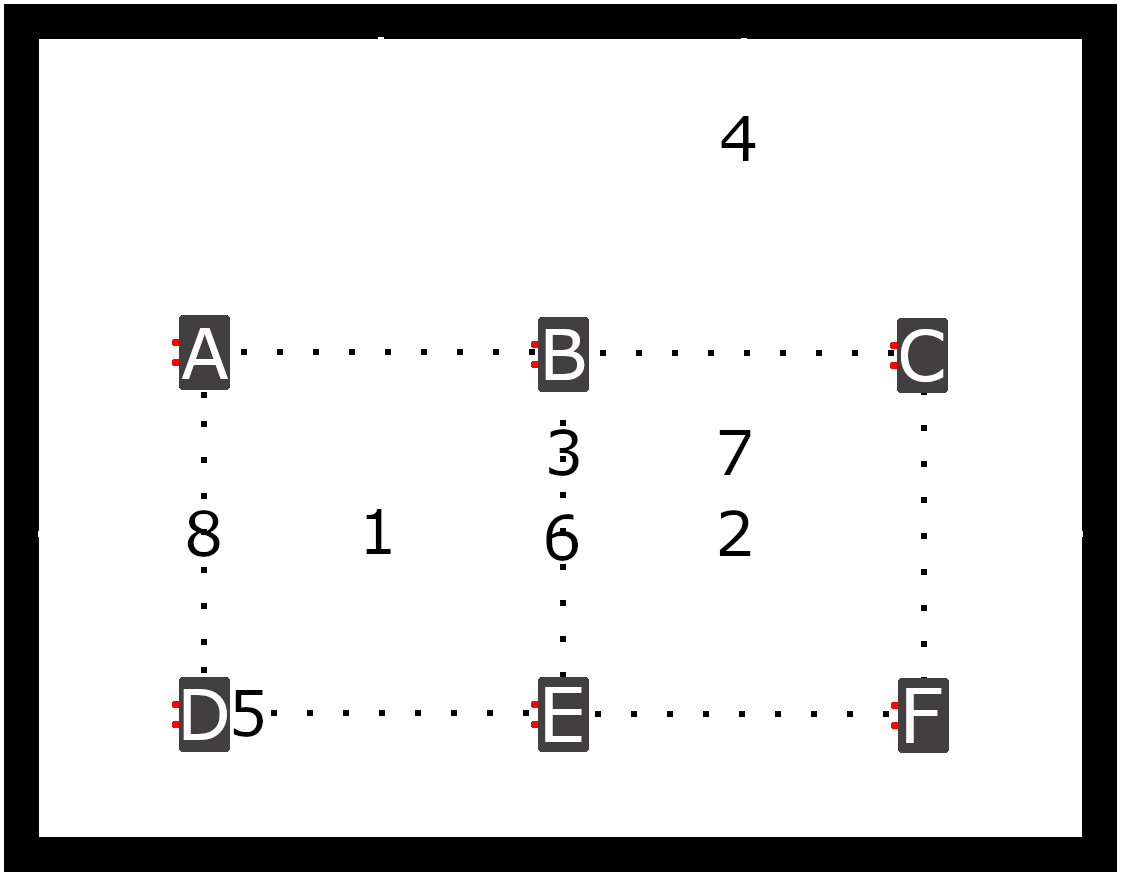
\includegraphics[width=\linewidth]{sble_2_1_floor}
	\captionof{figure}{Meerdere gateways per locatie - Opstelling 1}
	\label{fig:ond-ble-static-2-1-ops}
\end{minipage}

\paragraph{Resultaat}
Bij dit scenario gebeurt de toewijzing van een beacon aan een locatie aan de hand van de hoogste som van de RSSI waarden van de 4 omringende gateways van een locatie. Voor deze test zijn deze resultaten zichtbaar in tabel~\ref{fig:ond-ble-static-2-1-res} en deze zijn verrassend goed, met voor elke van de 8 beacons een correcte lokalisatie. Enkele interessante randgevallen zijn beacon 3 en 6, welke op de grens tussen de 2 locaties liggen. Bij beide zijn de cijfers duidelijk voor de rechtse locatie, nochtans is te verwachten dat deze cijfers dichter bijeen zouden liggen. Verder is er ook beacon 4, welke op geen enkele locatie ligt en is ingedeeld bij de rechtse locatie. Deze indeling is uiteindelijk de correcte, aangezien dit de dichtstbijzijnde locatie betreft en er geen 'geen locatie' mogelijk is in dit experiment. 
\begin{figure}[h]
	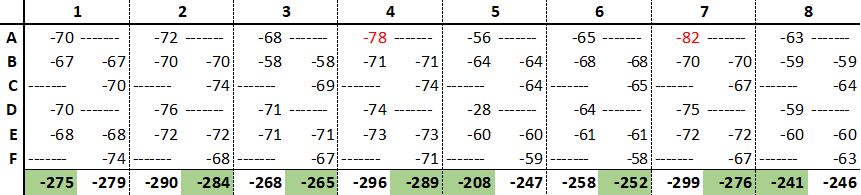
\includegraphics[width=\linewidth]{sble_2_1_results}
	\captionof{table}{Meerdere gateways per locatie - Testresultaat 1}
	\label{fig:ond-ble-static-2-1-res}
\end{figure}

\paragraph{Testconclusie}
Deze opstelling zorgt voor een perfecte lokalisatie in deze eerste, en is daarmee voorlopig zeer goed. Echter is er het detail van de 'geen locatie' beacons, maar dit is in elk scenario een ding. Hier is dit in theorie oplosbaar aangezien er een bepaalbare bovengrens is in de som van RSSI waarden wil de beacon nog tussen de gateways liggen. Deze is ook theoretisch berekenbaar gegeven de afstand tussen de gateways, de FSPL formule\footnote{Zie Sectie~\ref{sec:lit-definities} op pagina~\pageref{sec:lit-definities}} en enige meetkundige kennis. Echter door het vastgestelde verschil tussen theorie en praktijk tijdens het vooronderzoek lijkt dit eerder een maximum dat moet worden gemeten/bepaald.

\subsubsection{Test 2: 2 rechthoekige locaties gescheiden door muur}
\label{sec:ond-ble-2-2}
\begin{minipage}{0.55\textwidth}
De opstelling voor deze test is analoog aan de vorige, met als enige verschil dat er een muur is verschenen tussen de 2 locaties. Dit is weergegeven in figuur~\ref{fig:ond-ble-static-2-2-ops}. Dit ligt ook dichter bij de realiteit, nl. 2 aanpalende lokalen. Het doel van deze test is om het effect van deze muur op de cijfers te onderzoeken.
\end{minipage}
\hfill
\begin{minipage}{0.42\textwidth}
	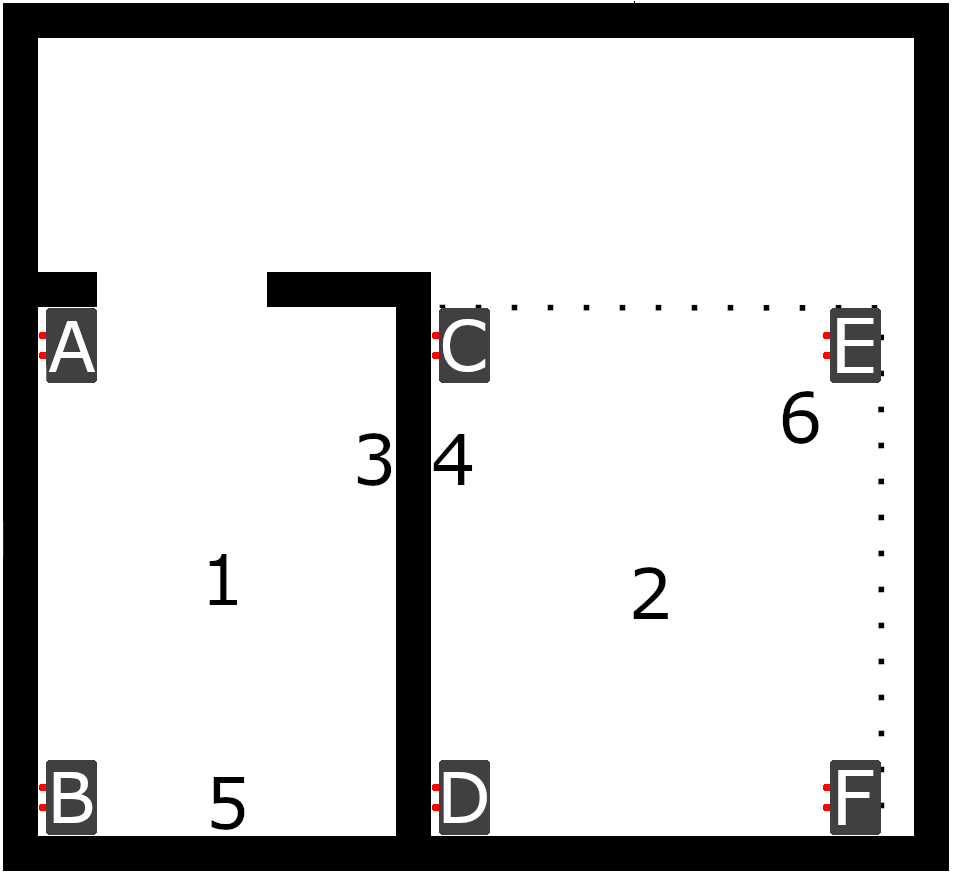
\includegraphics[width=\linewidth]{sble_2_2_floor}
	\captionof{figure}{Meerdere gateways per locatie - Opstelling 2}
	\label{fig:ond-ble-static-2-2-ops}
\end{minipage}

\paragraph{Resultaat}
In deze 2e test is dit scenario er ook weer in geslaagd elke beacon correct te lokaliseren, zoals zichtbaar in tabel~\ref{fig:ond-ble-static-2-2-res}. Hier is wel een extra stap bij de verwerking gekomen. Door het toevoegen van de muur wordt niet elke beacon door elke gateway meer opgevangen. Dit wordt weergegeven door een rode, platte streep in de tabel. Het spreekt voor zich dat dit ook meteen diskwalificerend werkt voor de locatie(s) waarvan deze gateway een hoekpunt is aangezien de beacon niet tussen deze gateways zal liggen als er 1 van deze gateways de beacon niet eens ziet.

\begin{figure}[h]
	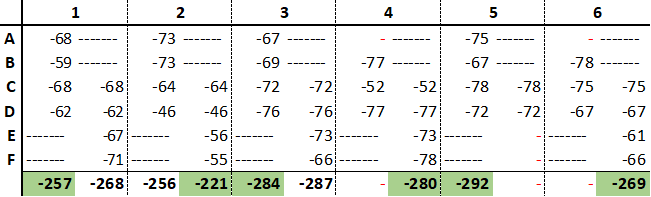
\includegraphics[width=\linewidth]{sble_2_2_results}
	\captionof{table}{Meerdere gateways per locatie - Testresultaat 2}
	\label{fig:ond-ble-static-2-2-res}
\end{figure}

\paragraph{Testconclusie}
Op het eerste zicht lijkt deze test volledig geslaagd, het toevoegen van een muur zorgt er niet voor dat dit scenario slechter presteert. Echter is er wel een belangrijk detail dat aangehaald moet worden. Als de cijfers beter onderzocht worden blijkt het volgende: bij elke beacon is de gateway die hem met de hoogste RSSI waarneemt een gateway die in dezelfde ruimte ligt als de beacon. Met andere woorden dezelfde uitkomst kan bekomen worden met 1 gateway per ruimte, en zo wordt de opstelling vereenvoudigd tot het scenario behandeld in sectie~\ref{sec:ond-ble-1}. Daarvoor zijn ook minder gateways nodig, waardoor ze beter is dan dit scenario qua hardware kost.

\subsubsection{Deelconclusie}
Dit scenario blijkt zeer effectief te zijn en heeft alle geteste beacons perfect gelokaliseerd. Echter blijkt wel dat deze opstelling geen voordelen heeft over de vorige (1 gateway / locatie) als een locatie ommuurd is, maar wel meer hardware vereist. Hiervoor is het niet geschikt. Voor lokalisatie in een open ruimte echter, lijkt ze beter te werken, voor een hogere hardware kost. De deelhypothese is aangenomen.

\subsection{Gateways in rasteropstelling}
\label{sec:ond-ble-3}
\subsubsection{Deelhypothese}
Deze opstelling is in staat om verspreide, getagde assets te detecteren en eenduidig aan de correcte locatie toe te wijzen.

\subsubsection{Test 1: Raster in open, reële ruimte}
\label{sec:ond-ble-3-1}
\begin{minipage}{0.55\textwidth}
De opstelling voor deze test is analoog aan de opstelling van test 1 in sectie~\ref{sec:ond-ble-1}, zoals zichtbaar in figuur~\ref{fig:ond-ble-static-3-1}. Bij deze opstelling zijn geen specifieke locaties gedefinieerd. Het is hier eerder de bedoeling om via trilateratie te bepalen waar een beacon zich exact bevind, en zo een toewijzing te doen naar de locatie die dat punt bevat. Wat de exacte lay-out van de locaties is is hiervoor irrelevant. Aangezien bij test 1 in sectie~\ref{sec:ond-ble-1} ook beacons in een raster gemeten zijn, kon de data uit die test hier hergebruikt worden en worden verwerkt met trilateratie. 
\end{minipage}
\hfill
\begin{minipage}{0.42\textwidth}
	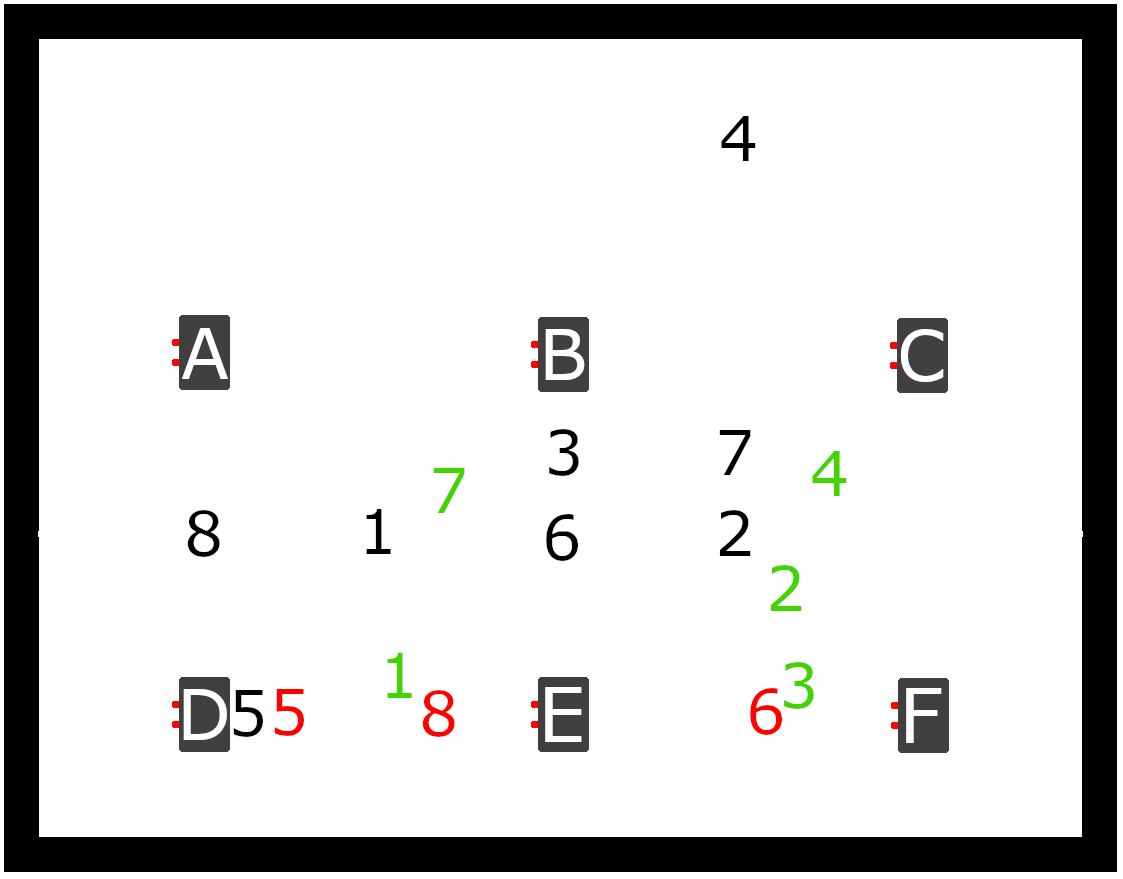
\includegraphics[width=\linewidth]{sble_3_1_floor}
	\captionof{figure}{Gateways in rasteropstelling - Test 1}
	\label{fig:ond-ble-static-3-1}
\end{minipage}

Voordat trilateratie\footnote{Zie Sectie~\ref{sec:lit-definities} op pagina~\pageref{sec:lit-definities}} kan toegepast worden, moet er eerst een omzetting gebeuren tussen de RSSI waarden en de afstand. Dit kan door de FSPL formule\footnote{Zie Sectie~\ref{sec:lit-definities} op pagina~\pageref{sec:lit-definities}} te gebruiken (weliswaar omgekeerd). Aangezien bij de verwerking van de resultaten op deze manier blijkt dat dit ver van correct is wordt er nog een offset in dBm toegevoegd, verschillend per soort beacon. Dit om het bij het vooronderzoek vastgelegde fenomeen dat beacons, hoewel ze de zelfde instellingen hebben, niet allen een even sterk signaal sturen. Bij de verwerking is een waarde gebruikt van -16 dBm voor de gebruikte H5 beacons, en -10 dBm voor de M2 beacons. Deze waarden zijn experimenteel vastgelegd, en vloeien voort uit de data van de afstandstest bij het vooronderzoek, waar de offset van de trendlijn tegenover de theoretische curve is gebruikt.

De resultaten van de trilateratie zijn geplot op het grondplan in figuur~\ref{fig:ond-ble-static-3-1}. De zwarte cijfers zijn de effectieve locaties van de beacons. De gekleurde zijn de berekende locaties a.d.h.v. de resultaten en trilateratie, met de groene een geslaagde trilateratie, en een rode een mislukte. Een mislukte wilt zeggen dat trilateratie niet mogelijk is door te korte afstanden (bv. de afstand tussen beacon 6 en gateway E en F bedraagt resp. 0.87m en 0.62m, opgeteld 1.49m. Dit is onmogelijk aangezien de afstand tussen deze gateways 2m bedraagt). Bij een situatie zoals deze is de beacon geplaatst tussen de 2 gateways.

\paragraph{Resultaat}
Om het resultaat te berekenen zijn de 2 gateways met de beste RSSI gebruikt. Meteen is zichtbaar dat het resultaat vrij catastrofaal is en dat de uitkomst van de trilateratie de beacons precies random plaatst. Beacon 5 komt in de buurt, maar deze lag fysiek aan gateway 5, waardoor zijn RSSI zeer hoog was (-28 dBm), hierdoor werd deze door de noodoplossing van het algoritme toch ietwat in de buurt geplaatst maar dit is een unicum. Verder is enkel beacon 2 vrij goed geplaatst.

\paragraph{Testconclusie}
Het is duidelijk dat trilateratie op basis van RSSI zeer onnauwkeurig is. Dit ligt vooral aan het onnauwkeurig omzetten van RSSI waardes in afstanden door de grote onzekerheden op RSSI waardes. Deze eerste test belooft zeker niet veel goeds voor dit concept.

\subsubsection{Test 2: Raster verspreid over gebouw met muren}
\label{sec:ond-ble-3-2}
\begin{minipage}{0.55\textwidth}
In deze 2e test is het raster vergroot, van 2m maar 3.5m tussen gateways. Ook is het raster verspreid over een gebouw, met muren tussen. De methodieken voor berekening en de kleurcodes voor het visualiseren van de resultaten zijn gelijk gebleven aan test 1 en dit alles is zichtbaar in figuur~\ref{fig:ond-ble-static-3-2}.
\end{minipage}
\hfill
\begin{minipage}{0.42\textwidth}
	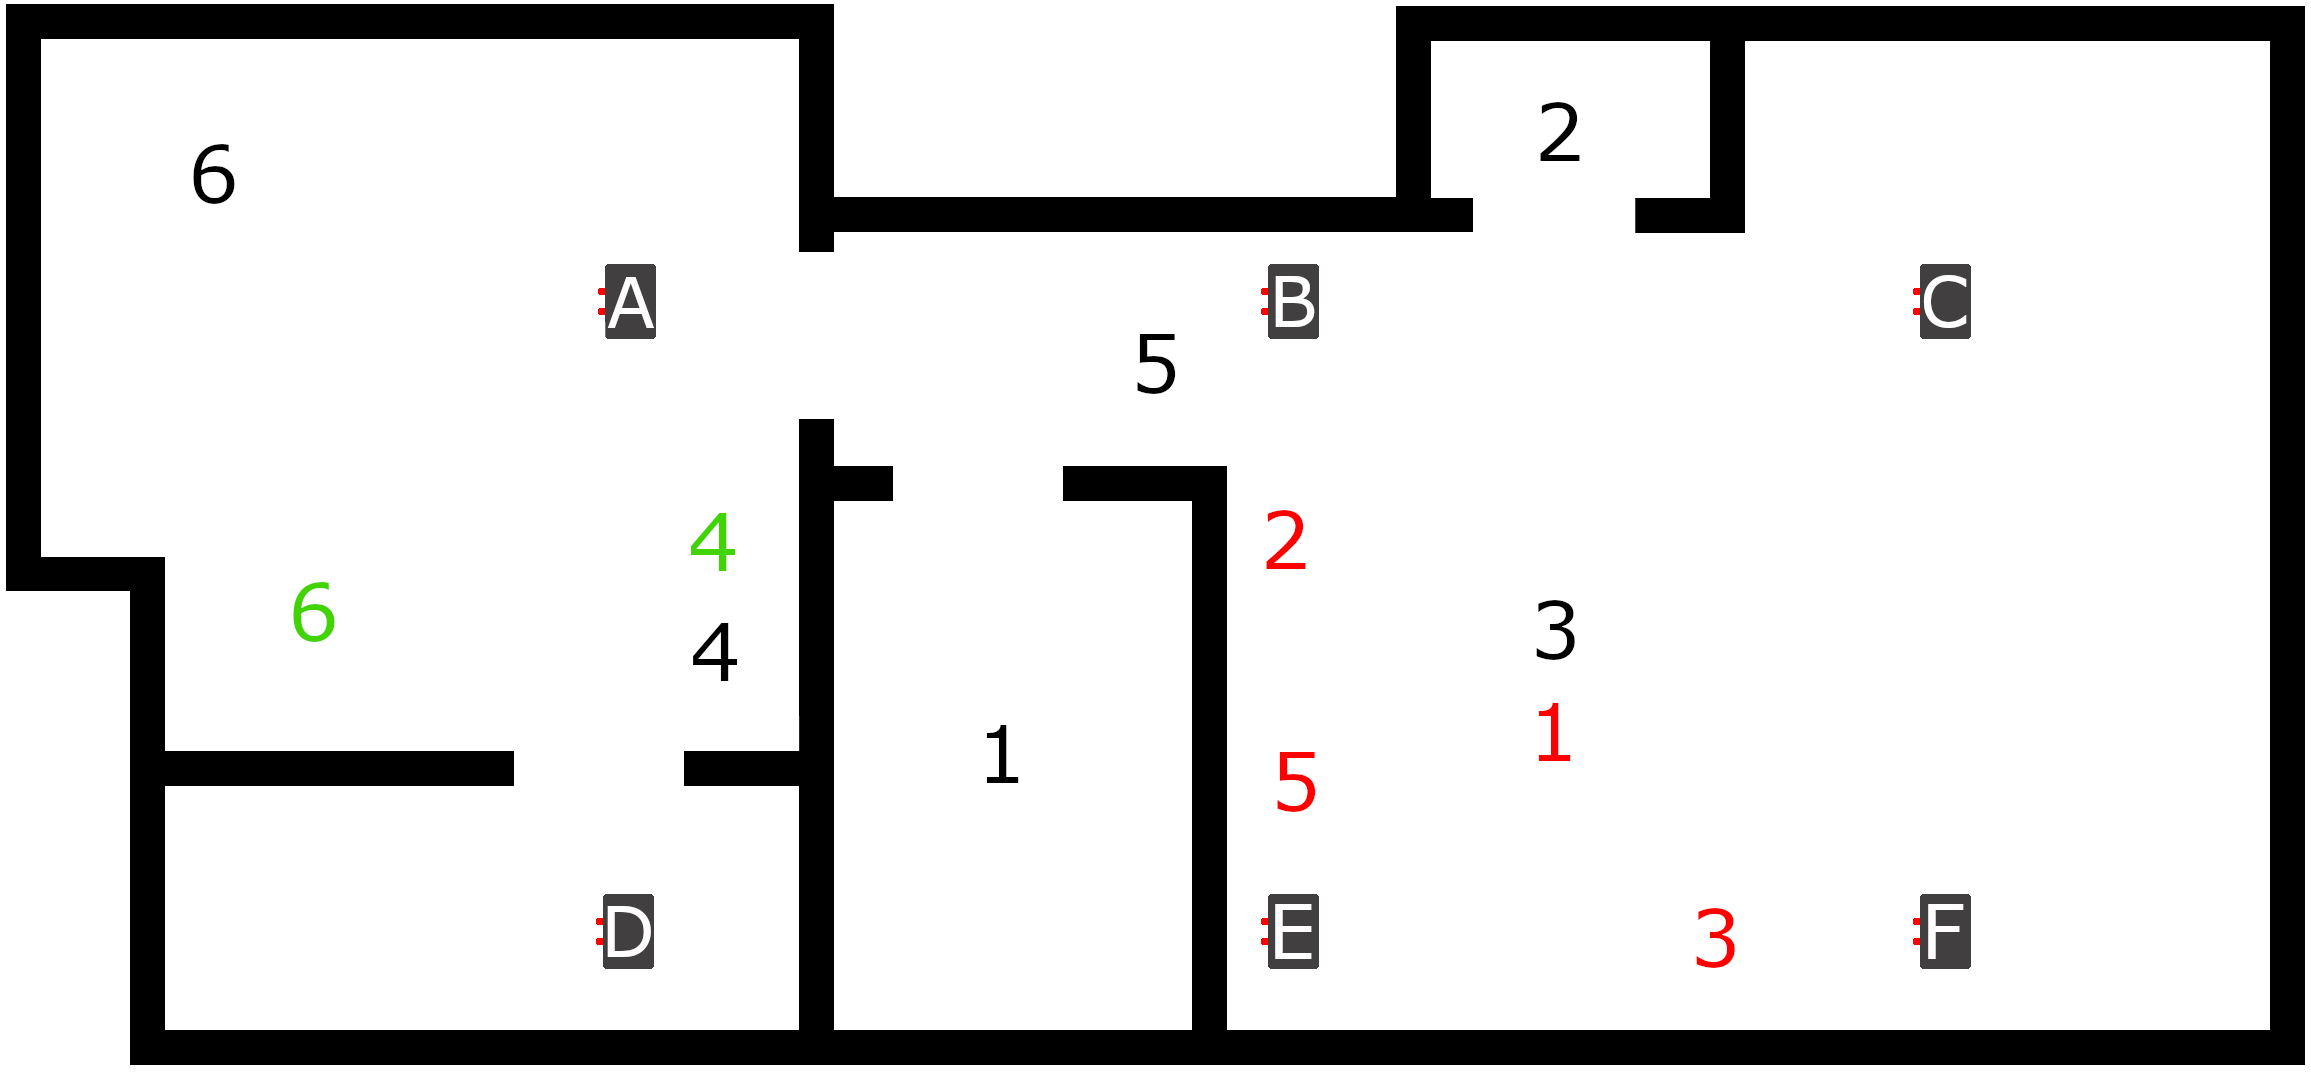
\includegraphics[width=\linewidth]{sble_3_2_floor}
	\captionof{figure}{Gateways in rasteropstelling - Opstelling 2}
	\label{fig:ond-ble-static-3-2-ops}
\end{minipage}

\paragraph{Resultaat}
\begin{minipage}{0.55\textwidth}
Na deze test zijn er slechts 2 beacons die met succes kunnen getrilatereerd worden zonder de noodoplossing te gebruiken (groen). Deze 2 beacons (4 en 6) zijn ook enkel opgemerkt door de 2 gateways waar ze tussen liggen. De 4 andere beacons zijn zeer slecht geplaatst in vergelijking met hun effectieve positie.
\end{minipage}
\hfill
\begin{minipage}{0.42\textwidth}
	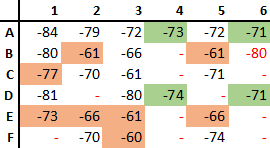
\includegraphics[width=\linewidth]{sble_3_2_results}
	\captionof{table}{Gateways in rasteropstelling - Testresultaat 2}
	\label{fig:ond-ble-static-3-2-res}
\end{minipage}

\paragraph{Testconclusie}
Deze grotere test heeft weer aangetoond wat na vorige test al duidelijk was, trilateratie op basis van RSSI is onnauwkeurig. En het toevoegen van muren, waardoor niet elke gateway meer elke beacon detecteert, verslecht de nauwkeurigheid enkel.

\subsubsection{Deelconclusie}
Na deze 2 tests kan duidelijk worden besloten dat dit scenario niet haalbaar is met de gebruikte BLE hardware. In het principe zit potentieel, maar enkel als er een goeie, precieze conversie kan worden gemaakt tussen RSSI waardes en afstanden. De deelhypothese is verworpen.
Een eventuele andere oplossing is het omzeilen van de RSSI naar afstand omrekening door een systeem van verhoudingen tussen RSSI waardes om de beacon naar een gateway 'toe te trekken' als het ware. Het is mogelijk dat een geschikter algoritme bestaat voor het bepalen van de locatie van een beacon in een gateway raster, niet gebaseerd op trilateratie. Dit valt echter buiten de beschouwde opstellingen, en ook buiten de eerder verkennende scope van dit onderzoek waardoor hier niet verder op wordt ingegaan.

\section{Dynamische BLE}
In tegenstelling tot bij de statische BLE opstellingen, is de variabele 'tijd' wel belangrijk bij dynamische BLE opstellingen. Daarom is het essentieel dat de tijd tussen de berichten, ontvangen van de gateway, vrij kort is. Een tussenperiode van 30s is hierbij niet wenselijk, aangezien de gateway zich zeer ver kan verplaatsten in deze tijdspanne en de metingen vrijwel nutteloos zullen zijn. Vandaar dat de instellingen van zowel de beacons als de gateway zullen worden versneld tijdens volgende testen. De gateway zal elke seconde zijn gemeten informatie doorsturen. Verder is het bij deze snelheden niet meer mogelijk om een beacon zendsnelheid van 30 berichten per gatewaybericht aan te houden aangezien de maximale snelheid 10 berichten/seconde bedraagt. Deze maximumsnelheid zal ook worden gebruikt tijdens volgende testen.

\subsection{1 locatiebeacon per locatie, midden van locatie}
\label{sec:ond-ble-4}
\subsubsection{Deelhypothese}
Deze opstelling is in staat om verspreide, getagde assets te detecteren en eenduidig aan de correcte locatie toe te wijzen.

\subsubsection{Test 1: 3 even grote locaties in open reële ruimte}
\label{sec:ond-ble-4-1}
\begin{minipage}{0.55\textwidth}
Voor deze eerste test is een open ruimte opgedeeld in een gang en 3 locaties, liggende naast elkaar en langs 1 kant van deze gang. Dit is zichtbaar in figuur~\ref{fig:ond-ble-dynamic-1-1-ops}. Alle locaties zijn even groot, en voorzien van een locatiebeacon (MokoSmart H5) in hun middelpunt, met een onderlinge afstand van 200cm. Verder liggen er diverse H5 en M2 beacons verspreid over de ruimte. Tijdens de test verplaatst een gateway zich aan een constante snelheid door de gang, aangegeven door de pijl op de illustratie. De test duurt 20sec, en op deze tijd overbrugt de gateway de volledige breedte van de opstelling. 
\end{minipage}
\hfill
\begin{minipage}{0.42\textwidth}
	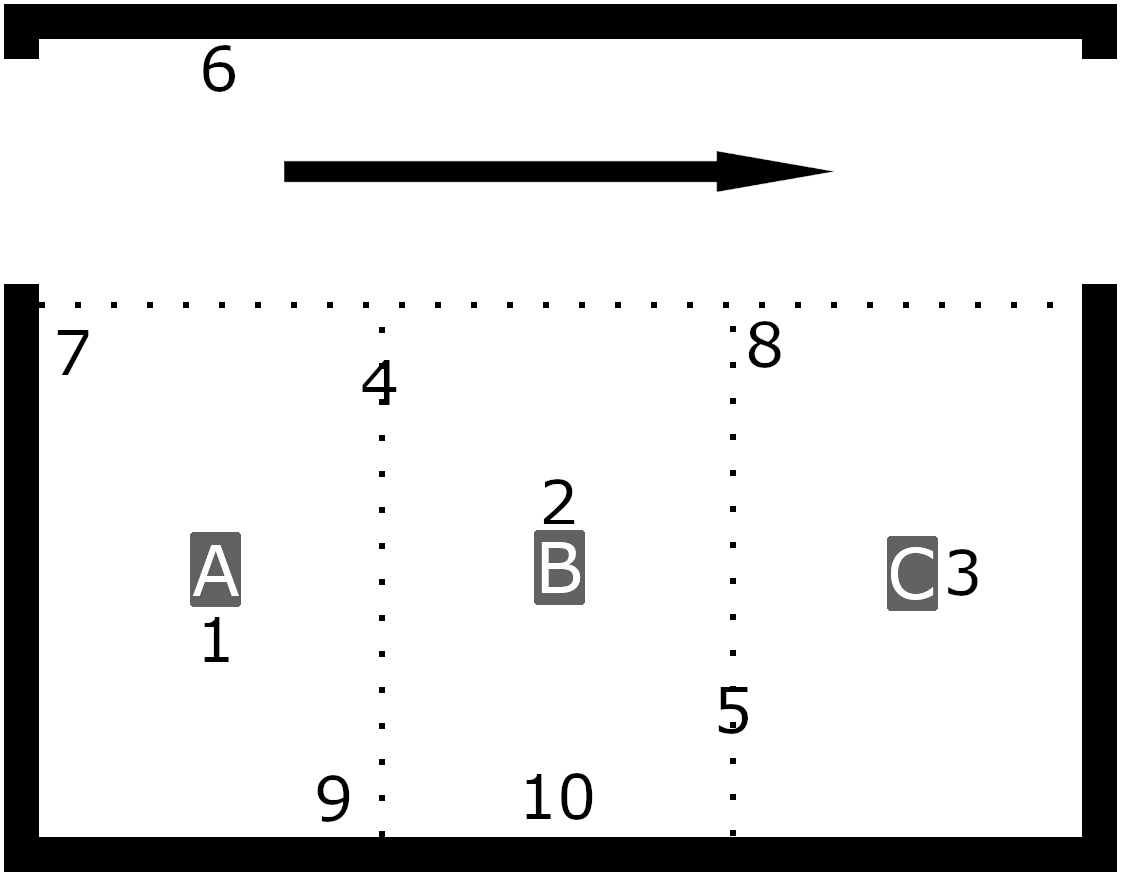
\includegraphics[width=\linewidth]{dble_1_1_floor}
	\captionof{figure}{1 beacon per locatie, midden van locatie - Opstelling 1}
	\label{fig:ond-ble-dynamic-1-1-ops}
\end{minipage}

\paragraph{Resultaat}
\begin{minipage}{0.42\textwidth}
In tabel~\ref{fig:ond-ble-dynamic-1-1-res} zijn de resultaten van deze test zichtbaar. Elke kolom stelt een beacon voor, opgedeeld volgens locatie- en assetbeacons. Voor elke beacon is zijn maximale RSSI waarde aangeduid in groen. Dit punt komt overeen met het moment dat de gateway deze beacon het dichtste nadert en komt overeen met het moment dat de gateway de beacon voorbij komt. Hieruit kan afgeleid worden welke beacons bij elkaar in de buurt liggen. 
\end{minipage}
\hfill
\begin{minipage}{0.55\textwidth}
	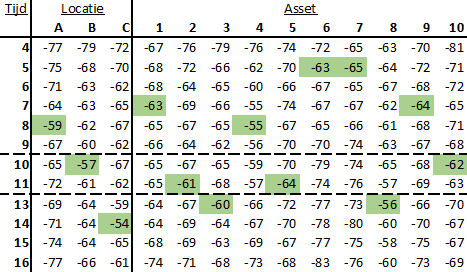
\includegraphics[width=\linewidth]{dble_1_1_results}
	\captionof{table}{1 beacon per locatie, midden van locatie - Testresultaat 1}
	\label{fig:ond-ble-dynamic-1-1-res}
\end{minipage}

De toewijzing van assetbeacons aan een locatie gebeurt volgens kleinste tijdverschil (een assetbeacon wordt toegewezen aan de locatie waarbij het tijdsverschil tussen zichzelf en de locatiebeacon van die locatie het kleinste is). In tabel~\ref{fig:ond-ble-dynamic-1-1-res} is een onderbroken lijn geplaatst die deze toewijzingen weergeeft.

Vervolgens is uit deze resultaten te concluderen dat deze manier van lokaliseren verrassend goed werkt aangezien elk asset aan de correcte locatie is toegewezen. Beacon 4 en 5 bevinden zich op de grens tussen 2 locaties, en dit is ook zichtbaar aan de resultaten, aangezien hun maximale RSSI dicht bij een overgangslijn valt. Als louter wordt gekeken naar de volgorde zijn er hier en daar enkele onnauwkeurigheden. Dit is zichtbaar bij bv. beacons 4 en 9, maar dit verschil is eerder beperkt en verwaarloosbaar als er enkel interesse bestaat voor een locatietoewijzing.

\paragraph{Testconclusie}
Deze eerste test is veelbelovend. Met een zeer eenvoudig lokalisatiealgoritme, gebaseerd op de maximale RSSI waarde, kan een zeer accurate lokalisatie bekomen worden. Wel is het zo dat deze hoogste waardes bij de locatiebeacons vrij dicht bij elkaar liggen, dit vermoedelijk omdat deze beacons dieper in de ruimte liggen en het relatieve afstandsverschil tussen de gateway en de locatiebeacons niet zeer uitgesproken is. Dit zou kunnen vergroot worden door deze beacons dichter naar het gangpad te brengen, of door de gateway nog sneller te laten sturen.

\subsubsection{Test 2: gang omringd door 4 locaties van variabele grootte}
\label{sec:ond-ble-4-2}
\begin{minipage}{0.55\textwidth}
Deze test maakt gebruik van 4 locaties in verschillende groottes, gescheiden door muren, om zo een realistische gang te bekomen. Dit is zichtbaar op figuur~\ref{fig:ond-ble-dynamic-1-2-ops}. Verder bevinden deze locaties zich langs beide zijden van de gang. Voor de rest is deze opstelling analoog aan test 1.
\end{minipage}
\hfill
\begin{minipage}{0.42\textwidth}
	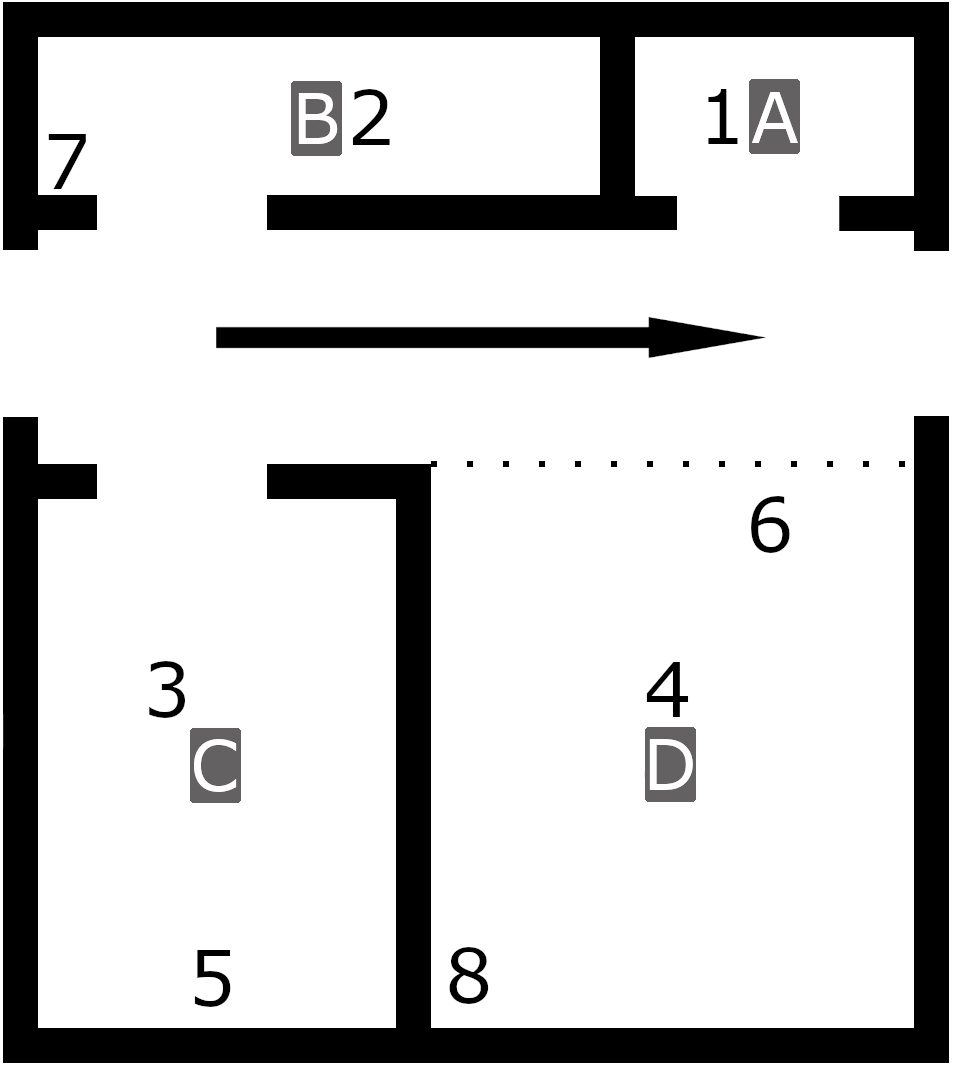
\includegraphics[width=\linewidth]{dble_1_2_floor}
		\captionof{figure}{1 beacon per locatie, midden van locatie - Opstelling 2}
	\label{fig:ond-ble-dynamic-1-2-ops}
\end{minipage}

\paragraph{Resultaat}
\begin{minipage}{0.42\textwidth}
Tabel~\ref{fig:ond-ble-dynamic-1-2-res} toont de resultaten van deze test, volgens dezelfde regels en opbouw als bij test 1. Als eerste valt op dat hier slechts 1 scheidingslijn aanwezig is. Dit is bewust. Bij deze test is het zo dat er locaties aanwezig zijn langs beide kanten van de gang, op ongeveer dezelfde hoogte. 
\end{minipage}
\hfill
\begin{minipage}{0.55\textwidth}
	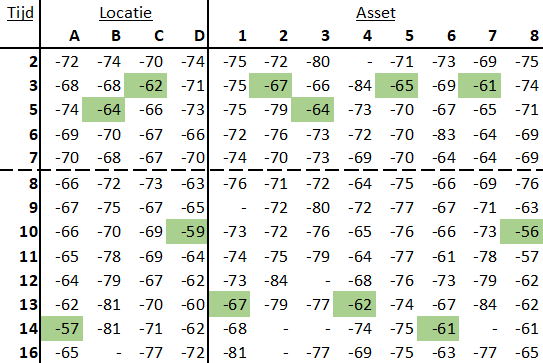
\includegraphics[width=\linewidth]{dble_1_2_results}
	\captionof{table}{1 beacon per locatie, midden van locatie - Testresultaat 2}
	\label{fig:ond-ble-dynamic-1-2-res}
\end{minipage}

Met 1 MikroTik KNOT gateway is het niet mogelijk richting (links of rechts) te detecteren en bijgevolg volgt er een samensmelting van deze 2 locaties. Na de vereenvoudiging door deze hardware limitatie blijven er 2 locaties over. De toewijzing van de assets aan deze 2 locaties is echter wel weer perfect gebeurd, en ook de volgorde zit nagenoeg correct.

\paragraph{Testconclusie}
Na deze 2e realistischere test, met toevoeging van muren, is er zichtbaar aan de resultaten dat de lokalisatie even goed (perfect) gebeurt als in de eenvoudigere opstelling van test 1. Wel is het duidelijk dat een links/rechts opdeling handig zou zijn voor een bruikbaarder resultaat, maar dit is enkel hardwarematig op te lossen. Bijvoorbeeld door het gebruik van 2 vlakke antennes, 1 naar rechts en 1 naar links gericht. Dit kan echter gesimuleerd worden door de resultaten op te delen in 2 (1 per richting), en het is duidelijk dat de resultaten in dat geval ook in orde zijn.

\subsubsection{Deelconclusie}
Uit deze testen is af te leiden dat dit principe van opstelling in alle gevallen zeer goed werkt, zowel in een open ruimte als met de toevoeging van muren. De deelhypothese is aangenomen.
	
\subsection{1 locatiebeacon per locatie, aan deur}
\label{sec:ond-ble-5}
\subsubsection{Deelhypothese}
Deze opstelling is in staat om verspreide, getagde assets te detecteren en eenduidig aan de correcte locatie toe te wijzen.

\subsubsection{Test 1: 3 even grote locaties in open ruimte}
\label{sec:ond-ble-5-1}
\begin{minipage}{0.55\textwidth}
De opstelling voor deze test is analoog aan de opstelling van test 1 uit sectie~\ref{sec:ond-ble-4}. De locatiebeacons zijn echter verplaatst van het midden van de locaties naar de grens tussen de locaties en de gang. Dit alles is zichtbaar in figuur~\ref{fig:ond-ble-dynamic-2-1-ops}.
\end{minipage}
\hfill
\begin{minipage}{0.42\textwidth}
	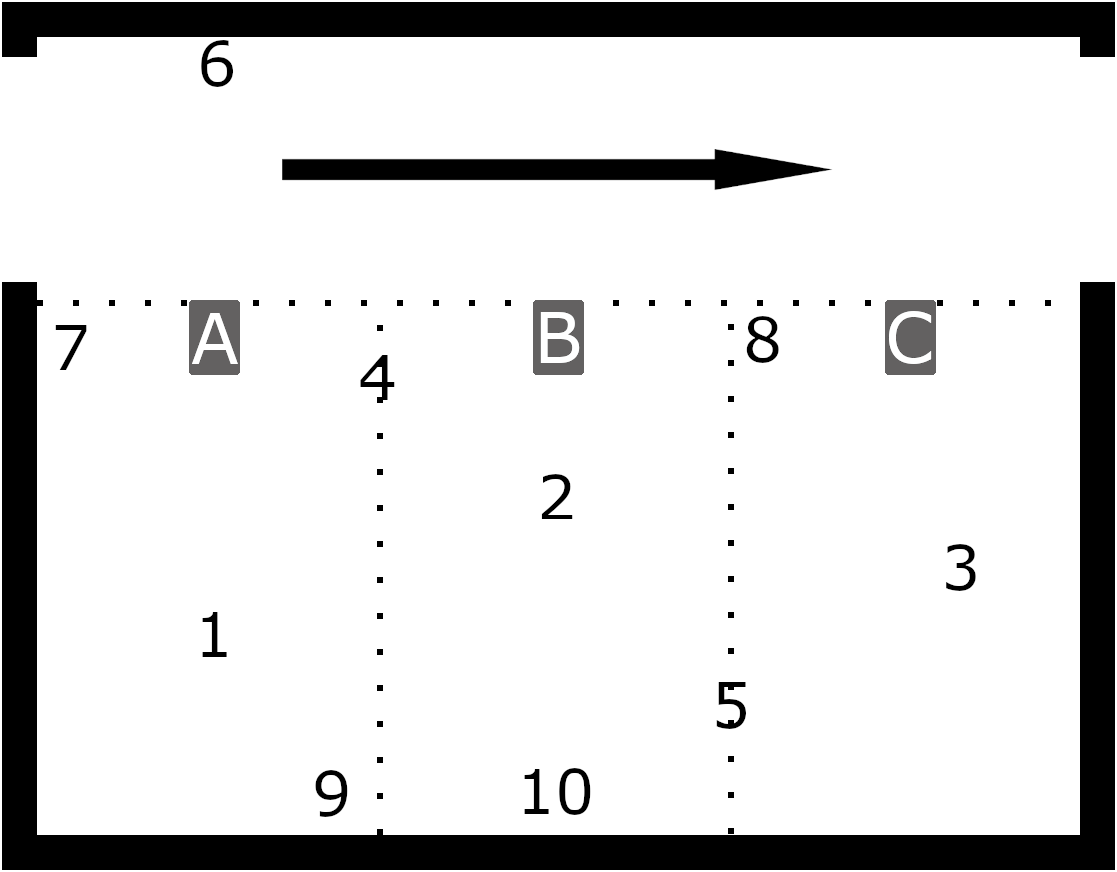
\includegraphics[width=\linewidth]{dble_2_1_floor}
	\captionof{figure}{1 beacon per locatie, aan deur - Opstelling 1}
	\label{fig:ond-ble-dynamic-2-1-ops}
\end{minipage}

\paragraph{Resultaat}
\begin{minipage}{0.42\textwidth}
De resultaten in tabel~\ref{fig:ond-ble-dynamic-2-1-res} zijn zeer analoog aan deze bij test 1 uit sectie~\ref{sec:ond-ble-4}. Met als enige verschil dat de locatiebeacons verder uit elkaar liggen in de tijd. Verder worden alle assets wederom correct gecategoriseerd per locatie, met een onderlinge volgorde van maximale RSSI waardes die ruwweg overeenkomt met de volgorde waarop de gateway de beacons is voorbij gekomen. 
\end{minipage}
\hfill
\begin{minipage}{0.55\textwidth}
	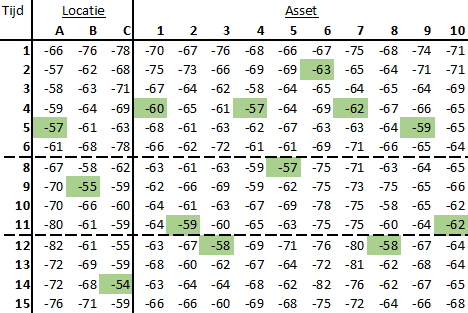
\includegraphics[width=\linewidth]{dble_2_1_results}
	\captionof{table}{1 beacon per locatie, aan deur - Testresultaat 1}
	\label{fig:ond-ble-dynamic-2-1-res}
\end{minipage}

Als opvallende uitzondering op deze volgorde is er tag 5, welke zeer hard naar voor gesprongen is in de volgorde. Wat nog maar eens onderstreept dat RSSI metingen niet precies zijn, en dat een combinatie van fenomenen zoals reflecties en stralingspatronen toevallige miscategorisaties kunnen veroorzaken, zoals vastgesteld tijdens het vooronderzoek. In deze test was dit niet het geval, maar de relatieve plaats van tag 5 is versprongen van op de grens tussen locatie B en C naar de grens tussen locatie A en B.

\paragraph{Testconclusie}
Deze test vertoont, buiten een betere spreiding van de locatiebeacons in de tijd, geen noemenswaardige verschillen met test 1 uit sectie~\ref{sec:ond-ble-4}.

\subsubsection{Test 2: gang omringd door 4 locaties van variabele grootte}
\label{sec:ond-ble-5-2}
\begin{minipage}{0.55\textwidth}
Deze test is analoog aan test 2 uit sectie~\ref{sec:ond-ble-4}, met als enige verschil dat de locatiebeacons niet geplaatst zijn in het middelpunt, maar aan de deur.
\end{minipage}
\hfill
\begin{minipage}{0.42\textwidth}
	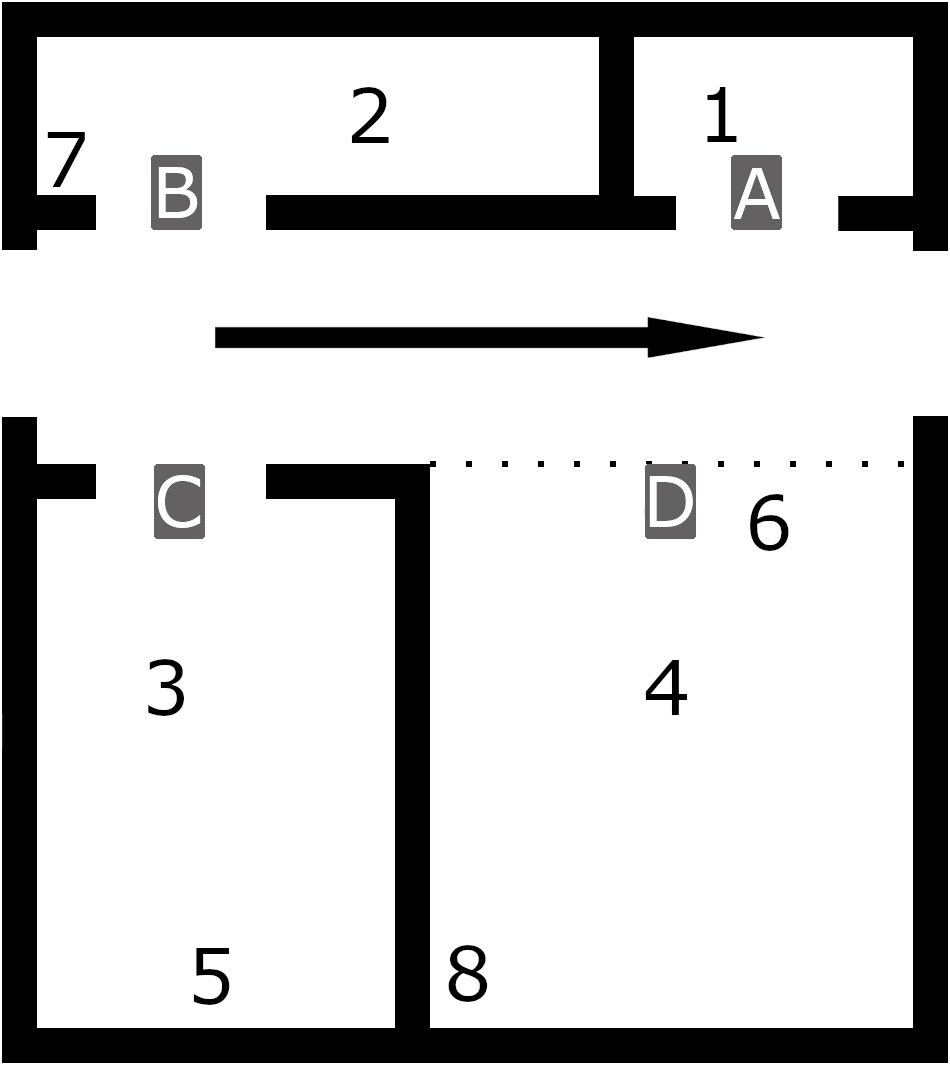
\includegraphics[width=\linewidth]{dble_2_2_floor}
	\captionof{figure}{1 beacon per locatie, aan deur - Opstelling 2}
	\label{fig:ond-ble-dynamic-2-2-ops}
\end{minipage}

\paragraph{Resultaat}
\begin{minipage}{0.42\textwidth}
Ook bij deze resultaten, zichtbaar in tabel~\ref{fig:ond-ble-dynamic-2-2-res}, zijn de verschillen met de overeenkomstige test in sectie~\ref{sec:ond-ble-4} beperkt. Het enige wat opvalt is dat de maximale RSSI-waardes van locatiebeacons B en C vrij veel zijn verhoogd, wat het gevolg is van de geografie. Locatiebeacon B ligt in dit geval niet meer achter een muur, en C ligt niet meer diep in een kamer, gecombineerd met een muur. 
\end{minipage}
\hfill
\begin{minipage}{0.55\textwidth}
	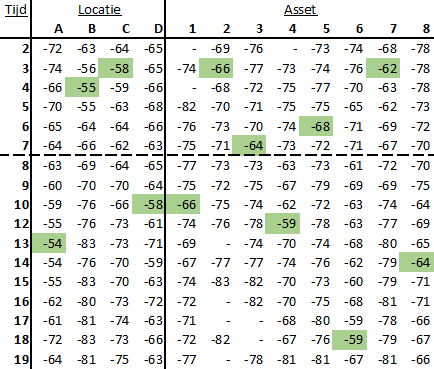
\includegraphics[width=\linewidth]{dble_2_2_results}
	\captionof{table}{1 beacon per locatie, aan deur - Testresultaat 2}
	\label{fig:ond-ble-dynamic-2-2-res}
\end{minipage}

\paragraph{Testconclusie}
Het lijkt erop dat het plaatsen van de locatiebeacons aan de deur in een realistische opstelling voordelen heeft tegenover in het midden van de kamer, voornamelijk op vlak van betere RSSI. Dit was niet het geval tijdens test 1 aangezien het effect van muren en deuren afwezig is in deze test. Verder is het wel zo dat een deur (zoals het geval bij beacon B) zich niet noodzakelijk in het midden van de locatie bevind. Dit heeft natuurlijk een effect op de toewijzing, aangezien de overgangslijn/tijd niet meer midden tussen de locatiebeacons moet geplaatst worden, maar verschoven wordt afhankelijk van de geografie van de locaties.

\subsubsection{Deelconclusie}
Dit scenario heeft een licht voordeel tegenover vorig scenario, maar enkel als het aankomt op een opstelling niet in een open ruimte. Het lijkt qua detectie en spreiding in de tijd beter om de locatiebeacons dichter bij de gang te hangen. De hypothese is aangenomen.

\subsection{Meerdere locatiebeacons per locatie}
\label{sec:ond-ble-6}
\subsubsection{Deelhypothese}
Deze opstelling is in staat om verspreide, getagde assets te detecteren en eenduidig aan de correcte locatie toe te wijzen.

\subsubsection{Test 1: 2 even grote locaties in open ruimte}
\label{sec:ond-ble-6-1}
\begin{minipage}{0.55\textwidth}
Voor deze test worden er in een open ruimte 2 locaties gecreëerd, met een locatiebeacon (MokoSmart H5) in elke hoek, waarvan bij de 2 overlappende hoeken een gemeenschappelijke locatiebeacon. Dit is zichtbaar in figuur~\ref{fig:ond-ble-dynamic-3-1-ops} Deze beacons liggen 2m uit elkaar. Ook zullen er assetbeacons verspreid worden, aangegeven door de cijfers op de figuur. Verder komt er een gateway voorbij volgens de richting van de pijl. 
\end{minipage}
\hfill
\begin{minipage}{0.42\textwidth}
	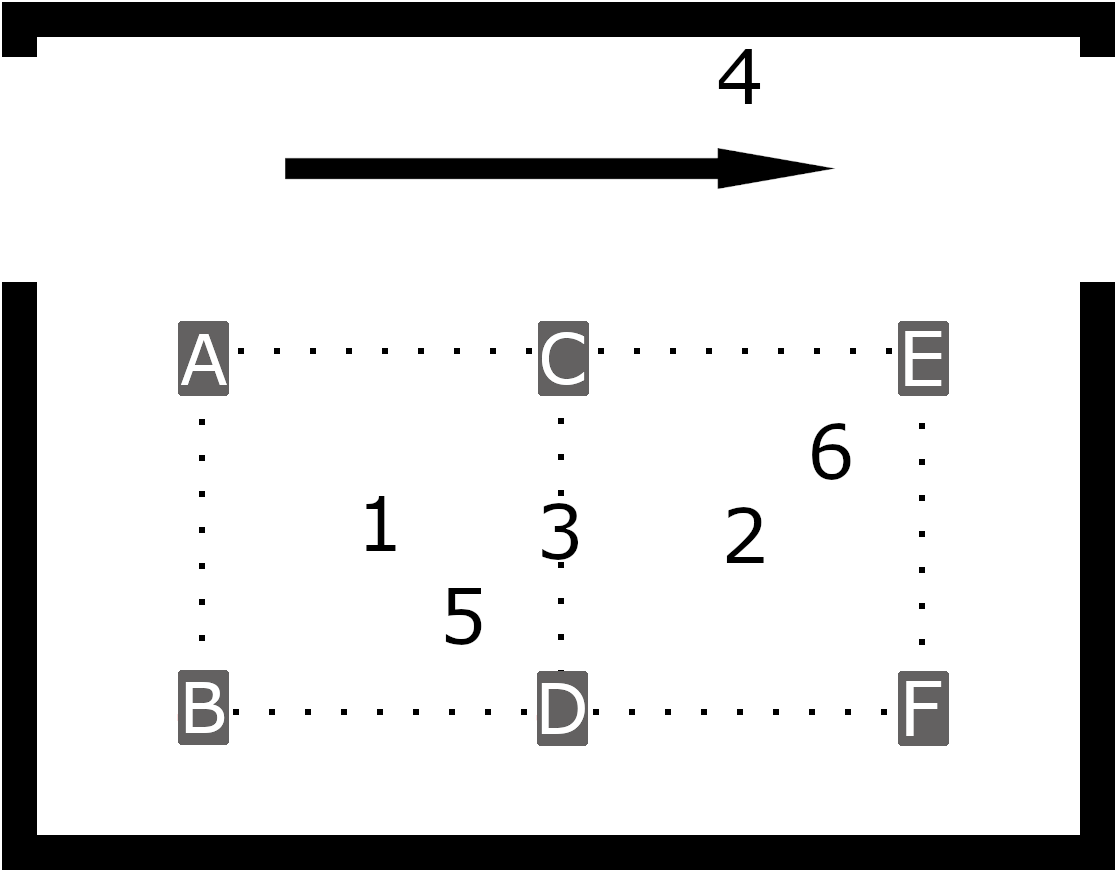
\includegraphics[width=\linewidth]{dble_3_1_floor}
	\captionof{figure}{Meerdere locatiebeacons per locatie - Opstelling 1}
	\label{fig:ond-ble-dynamic-3-1-ops}
\end{minipage}

\paragraph{Resultaat}
\begin{minipage}{0.42\textwidth}
Na het aggregeren en analyseren van de testdata ziet deze eruit zoals in tabel~\ref{fig:ond-ble-dynamic-3-1-res}. Hieruit valt zeer snel iets interessants op, als deze data verwerkt wordt door enkel te kijken naar de locatiebeacons die het dichtst tegen de gang aan liggen, en verder wordt gekeken naar de hoogste RSSI-waardes zoals in de vorige 2 scenario's klopt de lokalisatie perfect mits de grenslijn tegen de locatiebeacon wordt aangelegd. Dit wilt zeggen dat deze opstelling overbodig uitgebreid is en kan herleid worden tot het scenario uit sectie~\ref{sec:ond-ble-5}. 
\end{minipage}
\hfill
\begin{minipage}{0.55\textwidth}
	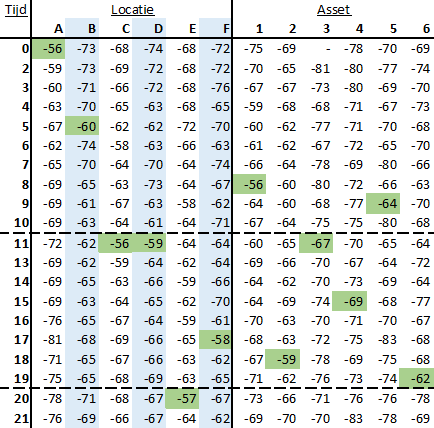
\includegraphics[width=\linewidth]{dble_3_1_results}
	\captionof{table}{Meerdere locatiebeacons per locatie - Testresultaat 1}
	\label{fig:ond-ble-dynamic-3-1-res}
\end{minipage}

Interessant is wel dat het ook mogelijk is om hetzelfde resultaat te bekomen met de achterste rij locatiebeacons (aangeduid in licht blauw in tabel~\ref{fig:ond-ble-dynamic-3-1-res}). Het is echter wel duidelijk dat deze punten dichter bij elkaar liggen in de tijd en minder nauwkeurig zullen zijn (zoals duidelijk het geval is met assetbeacon 2 en 6, welke in theorie buiten de locatie zouden vallen).

\paragraph{Testconclusie}
Dit scenario is overbodig complex en kan vereenvoudigd worden tot het vorige. Deze test heeft wel nogmaals bevestigd dat het voor de precisie beter is als de locatiebeacons dichter bij de gang liggen.

\subsubsection{Test 2: 2 even grote locaties gescheiden door muur}
\label{sec:ond-ble-6-2}
\begin{minipage}{0.55\textwidth}
In deze testopstelling is een muur toegevoegd tussen de 2 locaties van de testopstelling van test 1, zoals weergegeven in figuurtabel~\ref{fig:ond-ble-dynamic-3-2-ops}. Verder blijft de opstelling en test gelijk.
\end{minipage}
\hfill
\begin{minipage}{0.42\textwidth}
	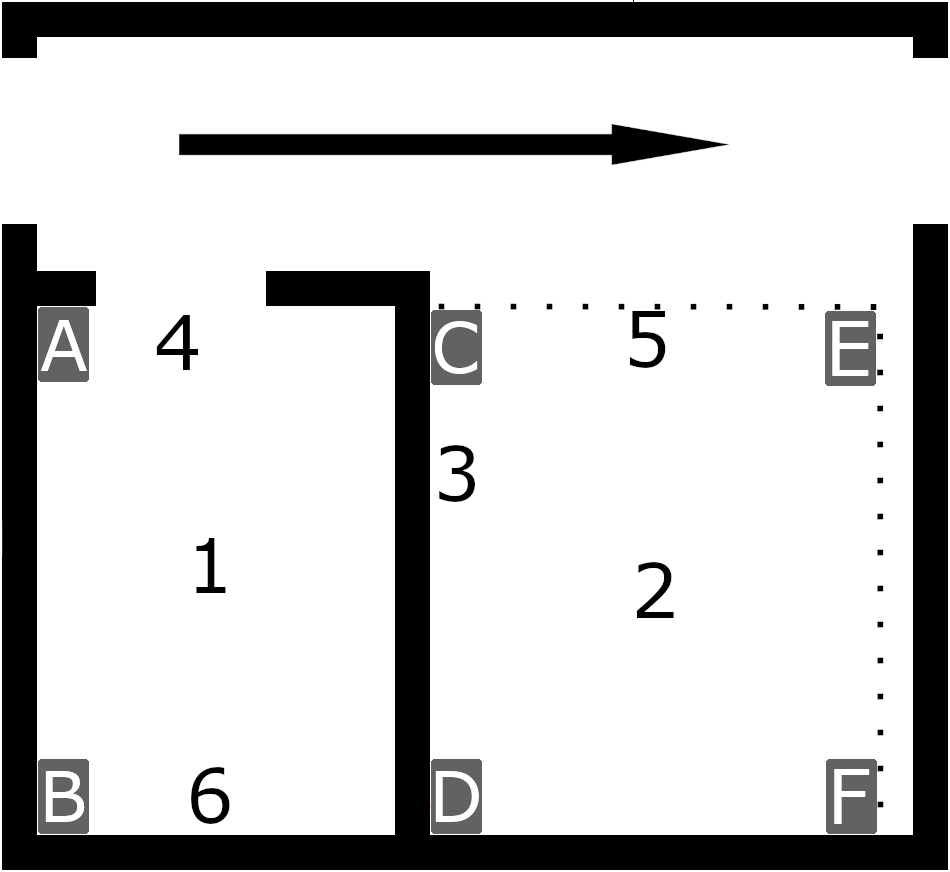
\includegraphics[width=\linewidth]{dble_3_2_floor}
	\captionof{figure}{Meerdere locatiebeacons per locatie - Opstelling 2}
	\label{fig:ond-ble-dynamic-3-2-ops}
\end{minipage}

\paragraph{Resultaat}
\begin{minipage}{0.42\textwidth}
Uit het resultaat van deze test, zichtbaar in tabel~\ref{fig:ond-ble-dynamic-3-2-res}, is hetzelfde al te leiden als uit de resultaten van test 1. De helft van de locatiebeacons blijkt overbodig en een herleiding naar het scenario uit sectie~\ref{sec:ond-ble-5} blijft mogelijk.
\end{minipage}
\hfill
\begin{minipage}{0.55\textwidth}
	\includegraphics[width=\linewidth]{dble_3_2_results}
	\captionof{table}{Meerdere locatiebeacons per locatie - Testresultaat 2}
	\label{fig:ond-ble-dynamic-3-2-res}
\end{minipage}

\paragraph{Testconclusie}
De toegevoegde muur heeft klaarblijkelijk geen effect op de resultaten, iets wat wel het geval was bij de statische versie van deze opstelling. Deze opstelling is wederom vereenvoudiggebaar naar die van het scenario uit sectie~\ref{sec:ond-ble-5}.

\subsubsection{Deelconclusie}
Na deze testen kan afgeleid worden dat dit scenario te ver gezocht is, en hetzelfde resultaat kan bereikt worden met een een eenvoudigere opstelling en minder hardware. Alhoewel te hypothese technisch gezien aangenomen is, zal dit scenario niet als beste uit de bus komen na dit onderzoek, door de overbodig hogere kostprijs.

\subsection{Locatiebeacons in rasteropstelling}
\label{sec:ond-ble-7}
\subsubsection{Deelconclusie}
Na de zeer slechte testresultaten van de statische versie van dit scenario in sectie~\ref{sec:ond-ble-3}, en omdat dit scenario zich qua principe berust op dubbele trilateratie, is besloten dit scenario niet nader te onderzoeken. Hierdoor zouden de extreme onnauwkeurigheden bij enkele trilateratie enkel maar extremer worden. 

\subsection{Locatiebeacons op intervallen in de gang}
\label{sec:ond-ble-8}
\subsubsection{Deelhypothese}
Deze opstelling is in staat om verspreide, getagde assets te detecteren en eenduidig aan de correcte locatie toe te wijzen.

\subsubsection{Test 1: 3 even grote locaties in open ruimte}
\label{sec:ond-ble-8-1}
\begin{minipage}{0.55\textwidth}
De opstelling voor deze test is gelijkaardig aan de opstelling van het test 1 uit het scenario uit sectie~\ref{sec:ond-ble-4}. Met als verschil dat de locaties niet meer 1 op 1 worden gedefinieerd door een locatiebeacon, maar dat deze locatiebeacons op gelijke afstand verspreid liggen in de gang (specifiek op 250cm onderlinge afstand). In deze opstelling bevinden de locatiegrenzen zich op resp. 2/3 de afstand tussen A en B, en op 1/3 de afstand tussen B en C. De rest van de afmetingen en opstelling zijn identiek. Dit alles is weergegeven in figuur~\ref{fig:ond-ble-dynamic-4-1-ops}.
\end{minipage}
\hfill
\begin{minipage}{0.42\textwidth}
	\includegraphics[width=\linewidth]{dble_4_1_floor}
	\captionof{figure}{Beacons op intervallen in de gang - Opstelling 1}
	\label{fig:ond-ble-dynamic-4-1-ops}
\end{minipage}

\paragraph{Resultaat}
\begin{minipage}{0.42\textwidth}
Ook de resultaten, zichtbaar in tabel~\ref{fig:ond-ble-dynamic-4-1-res}, zijn gelijkaardig aan deze in test 1 uit sectie~\ref{sec:ond-ble-4}. De plaatsing van de scheidingslijn tussen de verschillende locaties is echter wel verschillend. Aangezien de locatie van de locatiegrenzen en de beacons niet meer aan elkaar gelinkt zijn, hangt het af van de specifieke opstelling hoe deze zich tot elkaar verhouden. Hier is dit 2/3 en 1/3, en door recht evenredige verhouding tussen de afstand en de tijd door de constante snelheid is de scheidingslijn ook zo geplaatst in de tabel.
\end{minipage}
\hfill
\begin{minipage}{0.55\textwidth}
	\includegraphics[width=\linewidth]{dble_4_1_results}
	\captionof{table}{Beacons op intervallen in de gang - Testresultaat 1}
	\label{fig:ond-ble-dynamic-4-1-res}
\end{minipage}

Na deze andere manier van locatietoewijzing is het duidelijk dat de lokaliseringsresultaten nog steeds goed overeen komen met de werkelijkheid. Dit met uitzondering van beacon 1, welke is versprongen van de eerste naar de laatste locatie. Dit fenomeen is al tegengekomen in test 1 van sectie~\ref{sec:ond-ble-5} en wordt daar besproken.

\paragraph{Testconclusie}
Deze test vertoont analoge resultaten aan eerdere scenario's.

\subsubsection{Test 2: gang omringd door 4 locaties van variabele grootte}
\label{sec:ond-ble-8-2}
\begin{minipage}{0.55\textwidth}
De opstelling voor deze test is gelijkaardig aan deze uit test 2 in sectie~\ref{sec:ond-ble-4}. Idem aan test 1 worden de locatiebeacons geplaatst op gelijke afstanden in de tussenliggende gang. De locatieovergang tijdens deze test is vlak voor locatiebeacon B aan de rechterkant, en 1/3 de afstand tussen B en C langs de linkerkant van de gang.  Dit alles is weergegeven in figuur~\ref{fig:ond-ble-dynamic-4-2-ops}.
\end{minipage}
\hfill
\begin{minipage}{0.42\textwidth}
	\includegraphics[width=\linewidth]{dble_4_2_floor}
	\captionof{figure}{Beacons op intervallen in de gang - Opstelling 2}
	\label{fig:ond-ble-dynamic-4-2-ops}
\end{minipage}

\paragraph{Resultaat}
\begin{minipage}{0.42\textwidth}
Resultatentabel~\ref{fig:ond-ble-dynamic-4-2-res} is licht anders opgedeeld dan soortgelijke tabellen uit vorige tests, dit omdat er een opdeling is gemaakt tussen rechts en links van de gang. Dit is eenderzijds om een simulatie te maken voor een opstelling die een richting kan bepalen, en anderzijds omdat de definitie voor locatieovergang langs rechts en links verschilt. Bijgevolg is 1 lijn niet correct.
Er is duidelijk te zien in de resultaten dat de lokalisatie goed is gebeurt en elk asset in de juiste locatie is ingedeeld.
\end{minipage}
\hfill
\begin{minipage}{0.55\textwidth}
	\includegraphics[width=\linewidth]{dble_4_2_results}
	\captionof{table}{Beacons op intervallen in de gang - Testresultaat 2}
	\label{fig:ond-ble-dynamic-4-2-res}
\end{minipage}

\paragraph{Testconclusie}
Uit deze test is duidelijk dat ook in een reële situatie, assetbeacons in de gang een goede oplossing kan zijn.

\subsubsection{Deelconclusie}
Dit scenario heeft zeer gelijkaardige resultaten aan secties~\ref{sec:ond-ble-4} en~\ref{sec:ond-ble-5}. Het verschil met deze scenario's is echter wel dat bij deze niet elke locatie een beacon nodig heeft, en de hardware kost lager is. Ook is het mogelijk de locatiedefinitie te veranderen zonder de hardware te moeten verhangen, wat een voordeel kan geven voor sommige use cases. Langs de andere kant is wel een definitie nodig van waar een locatie start en eindigt, in relatie tot de locaties van de locatiebeacons. Dit zorgt voor een minder gestandaardiseerde uitrol van een systeem gebaseerd op dit scenario, en heeft hierdoor een hogere installatie en onderhoudskost.
